% ****************************************************************************************** % Dissertation template and document class for Princeton University
% Author  : Jeffrey Scott Dwoskin <jdwoskin@princeton.edu>
% Adapted from: http://www.math.princeton.edu/graduate/tex/puthesis.html
% ****************************************************************************************** %


%%% For print copies
%% set 'singlespace' option to set entire thesis to single space, and define "\printmode" to remove all hyperlinks for printed copies of the thesis. Delete all output files before changing this mode -- it will turn hyperref package on and off
%\documentclass[12pt,lot, lof, singlespace]{puthesis}
%\newcommand{\printmode}{}

%%% For the electronic copy, use doublespacing, define "\proquestmode" to use outlined links, instead of colored links. 
\documentclass[12pt,lot,lof,letterpaper]{puthesis}
\RequirePackage[letterpaper, left=1in, right=1in, top=1in, bottom=1in]{geometry}
\newcommand{\proquestmode}{}
\usepackage{fancyhdr}

% Define the page style with chapter headings
\fancypagestyle{myfancy}{%
  \fancyhf{} % Clear header/footer
  \renewcommand{\headrulewidth}{0pt} % Remove header rule
  \fancyhead[R]{\nouppercase\leftmark} % Chapter heading (not in all caps) on the right side of the header
  \fancyfoot[C]{\thepage} % Page number in the center of the footer
}
\usepackage{amsmath}
\usepackage{amsfonts}       % blackboard math symbols
\usepackage{booktabs}       % professional-quality tables
\usepackage{multirow}
% Apply the page style to all pages
\pagestyle{myfancy}

\usepackage{ccaption}
\usepackage{caption}
\usepackage[singlelinecheck=false]{caption}
\usepackage[justification=justified]{caption}
% Set the font size for figure captions
\captionsetup[figure]{font=small}
% I prefer proquestmode to be off for electronic copies for normal use, since the colored links are less distracting. However when printed in black and white, the colored links are difficult to read. 

%%% For early drafts without some of the frontmatter
% Also see the "ifodd" command below to disable more frontmatter
%\documentclass[12pt]{puthesis}

%%%%%%%%%%%%%%%%%%%%%%%%%%%%%%%%%%%%%%%%%%%%%%%%%%%%%%%%%%%%%\
%%%% Author & title page info

\title{Latent variable models for characterizing the dynamic structure underlying complex behaviors}

\submitted{September 2023}  % degree conferral date (January, April, June, September, or November)
\copyrightyear{2023}  % year in which the copyright is secured by publication of the dissertation.
\author{Iris Reid Stone}
\adviser{Professor Jonathan W. Pillow \& Professor Ilana B. Witten}  %replace with the full name of your adviser
\departmentprefix{}  % defaults to "Department of", but programs need to change this.
\department{Princeton Neuroscience Institute}

%%%%%%%%%%%%%%%%%%%%%%%%%%%%%%%%%%%%%%%%%%%%%%%%%%%%%%%%%%%%%\
%%%% Tweak float placements
% From: http://mintaka.sdsu.edu/GF/bibliog/latex/floats.html "Controlling LaTeX Floats"
% and based on: http://www.tex.ac.uk/cgi-bin/texfaq2html?label=floats
% LaTeX defaults listed at: http://people.cs.uu.nl/piet/floats/node1.html

% Alter some LaTeX defaults for better treatment of figures:
    % See p.105 of "TeX Unbound" for suggested values.
    % See pp. 199-200 of Lamport's "LaTeX" book for details.
    %   General parameters, for ALL pages:
    \renewcommand{\topfraction}{0.85}	% max fraction of floats at top
    \renewcommand{\bottomfraction}{0.6}	% max fraction of floats at bottom
    %   Parameters for TEXT pages (not float pages):
    \setcounter{topnumber}{2}
    \setcounter{bottomnumber}{2}
    \setcounter{totalnumber}{4}     % 2 may work better
    \setcounter{dbltopnumber}{2}    % for 2-column pages
    \renewcommand{\dbltopfraction}{0.66}	% fit big float above 2-col. text
    \renewcommand{\textfraction}{0.15}	% allow minimal text w. figs
    %   Parameters for FLOAT pages (not text pages):
    \renewcommand{\floatpagefraction}{0.66}	% require fuller float pages
	% N.B.: floatpagefraction MUST be less than topfraction !!
    \renewcommand{\dblfloatpagefraction}{0.66}	% require fuller float pages

% The documentclass already sets parameters to make a high penalty for widows and orphans. 

%%%%%%%%%%%%%%%%%%%%%%%%%%%%%%%%%%%%%%%%%%%%%%%%%%%%%%%%%%%%%\
%%%% Use packages

%\usepackage{amsfonts}

%%% For figures
\usepackage{graphicx}
%\usepackage{subfig,rotate}

%%% for comments
\usepackage{verbatim}

%%% For tables
\usepackage{multirow}
% Longtable lets you have tables that span multiple pages.
\usepackage{longtable}

% Booktabs produces far nicer tables than the standard LaTeX tables.
%   see: http://en.wikibooks.org/wiki/LaTeX/Tables
\usepackage{booktabs}

\bibliographystyle{unsrt}

%set parameters for longtable:
% default caption width is 4in for longtable, but wider for normal tables
\setlength{\LTcapwidth}{\textwidth}

\usepackage{titlesec}

% Set the font size for chapter titles
\titleformat{\chapter}[display]
  {\normalfont\LARGE\bfseries}{\chaptertitlename\ \thechapter}{1em}{}


% Set the font size for subsection titles
\titleformat{\subsection}{\normalsize\bfseries}{\thesubsection}{1em}{}

%%%%%%%%%%%%%%%%%%%%%%%%%%%%%%%%%%%%%%%%%%%%%%%%%%%%%%%%%%
%%% Printed vs. online formatting
\ifdefined\printmode

% Printed copy
% url package understands urls (with proper line-breaks) without hyperlinking them
\usepackage{url}
%\usepackage{amsmath}
\usepackage{amssymb}
\usepackage{mathtools}
\usepackage[upgreek, LGRgreek]{mathastext}

\else

\ifdefined\proquestmode
%ProQuest copy -- http://www.princeton.edu/~mudd/thesis/Submissionguide.pdf

% ProQuest requires a double spaced version (set previously). They will take an electronic copy, so we want links in the pdf, but also copies may be printed or made into microfilm in black and white, so we want outlined links instead of colored links.
\usepackage{hyperref}
\hypersetup{bookmarksnumbered}

% copy the already-set title and author to use in the pdf properties
\makeatletter
\hypersetup{pdftitle=\@title,pdfauthor=\@author}
\makeatother

\else
% Online copy

% adds internal linked references, pdf bookmarks, etc

% turn all references and citations into hyperlinks:
%  -- not for printed copies
% -- automatically includes url package
% options:
%   colorlinks makes links by coloring the text instead of putting a rectangle around the text.
\usepackage{hyperref}
\hypersetup{colorlinks,bookmarksnumbered}

% copy the already-set title and author to use in the pdf properties
\makeatletter
\hypersetup{pdftitle=\@title,pdfauthor=\@author}
\makeatother

% make the page number rather than the text be the link for ToC entries
%\hypersetup{linktocpage}
\fi % proquest or online formatting
\fi % printed or online formatting


%%%%%%%%%%%%%%%%%%%%%%%%%%%%%%%%%%%%%%%%%%%%%%%%%%%%%%%%%%%%%\
%%%% Define commands

% Define any custom commands that you want to use.
% For example, highlight notes for future edits to the thesis
%\newcommand{\todo}[1]{\textbf{\emph{TODO:}#1}}


% create an environment that will indent text
% see: http://latex.computersci.org/Reference/ListEnvironments
% 	\raggedright makes them left aligned instead of justified
\newenvironment{indenttext}{
    \begin{list}{}{ \itemsep 0in \itemindent 0in
    \labelsep 0in \labelwidth 0in
    \listparindent 0in
    \topsep 0in \partopsep 0in \parskip 0in \parsep 0in
    \leftmargin 1em \rightmargin 0in
    \raggedright
    }
    \item
  }
  {\end{list}}

% another environment that's an indented list, with no spaces between items -- if we want multiple items/lines. Useful in tables. Use \item inside the environment.
% 	\raggedright makes them left aligned instead of justified
\newenvironment{indentlist}{
    \begin{list}{}{ \itemsep 0in \itemindent 0in
    \labelsep 0in \labelwidth 0in
    \listparindent 0in
    \topsep 0in \partopsep 0in \parskip 0in \parsep 0in
    \leftmargin 1em \rightmargin 0in
    \raggedright
    }

  }
  {\end{list}}



%%%%%%%%%%%%%%%%%%%%%%%%%%%%%%%%%%%%%%%%%%%%%%%%%%%%%%%%%%%%%\
%%%% Front-matter

% For early drafts, you may want to disable some of the frontmatter. Simply change this to "\ifodd 1" to do so.
\ifodd 0
% front-matter disabled while writing chapters
\renewcommand{\maketitlepage}{}
\renewcommand*{\makecopyrightpage}{}
\renewcommand*{\makeabstract}{}

% you can just skip the \acknowledgements and \dedication commands to leave out these sections.

\else


\abstract{
% Abstract can be any length, but should be max 350 words for a Dissertation for ProQuest's print indicies (150 words for a Master's Thesis) or it will be truncated for those uses.
Latent variable models are a powerful tool for analyzing the dynamic structure underlying complex behavior in mammals. In this thesis, I discuss three applications of such models and demonstrate their utility in uncovering novel scientific insights in mice engaging in decision-making and exploratory behaviors. In the first, we use a hidden Markov model with generalized linear model observations (GLM-HMM) to discover that mice employ multiple internal states, or strategies, when performing a binary decision-making task. This work also reveals that the contribution of the dorsomedial striatum (DMS) to decision-making behavior is state-dependent. In the second application, we extend the use of latent variable models to high-dimensional, continuous-time naturalistic behavior, using a switching Linear Dynamical System (sLDS) to identify discrete states in mice openly exploring their environment. We find that this approach is superior to HMM-based methods in its ability to capture states that correspond to interpretable, consistent behavioral modules. Lastly, we detail novel approaches to improving inference in latent variable models, using ideas from spectral learning theory, with applications to both types of behavior. Overall, this work demonstrates the power of latent variable models to uncover hidden structure and insights into complex behavior in mice, which has broad implications for understanding neural circuits and behavior in both animal models and humans.
}

\acknowledgements{
%I would like to thank...
{\large \textbf{General acknowledgements}} \\
{\large \textbf{Additional acknowledgements for individual chapters}}\\
\textbf{Chapter 2} \\
First and foremost, I would like to thank my co-first author on the manuscript, Scott Bolkan, for his invaluable contributions to this project. He and Ilana conceived of the experimental work, and he performed all of the experiments and conducted substantial subsequent analysis on that data. The results of his efforts are reflected in the paper primarily in Sections \ref{sec:glmhmm:2.2.1} through \ref{sec:glmhmm:2.2.5}, in main Figures \ref{fig:glmhmm:1} through \ref{fig:glmhmm:3}, and in additional Figures \ref{fig:ap1:ext1}, \ref{fig:ap1:supp1}, \ref{fig:ap1:supp2}, \ref{fig:ap1:ext2}, \ref{fig:ap1:supp3}, \ref{fig:ap1:ext3}, \ref{fig:ap1:ext4}, \ref{fig:ap1:ext5}, \ref{fig:ap1:ext6}, \ref{fig:ap1:ext10}, \ref{fig:ap1:supp5}, and \ref{fig:ap1:supp6}. I also thank him for being a wonderful person to work with and a very supportive teammate; that support was crucial in my early years of graduate school. I also thank my other co-authors, the entire BRAINCoGs team, and the Pillow and Witten Labs for their feedback on the work, as well as the reviewers at \textit{Nature Neuroscience} for their helpful comments. \\
\textbf{Chapter 3} \\
As a computational neuroscientist, none of my work would be possible without the help of intrepid experimentalists who spend copious hours collecting data for me to explore. I am therefore endlessly grateful to Victoria Corbit, who designed the experimental setup, built the linear track chamber, collected all the video recordings, and performed the SLEAP keypoint labeling as described in Section \ref{sec:slds:3.2.1} and Figure \ref{fig:slds:1}. She was also a strong source of moral support and a great friend and teammate in the time that we worked together. I also acknowledge the support of Anna Zhukovskaya and Lindsay Willmore, who had their own projects studying naturalistic behavior in the Witten lab and offered me their insights, literature recommendations, and inspiration along the way. \\
\textbf{Chapter 4} \\
For this portion of my PhD work, I offer a huge round of acknowledgement to my co-first author Yotam Sagiv. Remember when we thought this would be a course project? What a special experience to work so closely on a paper with such a good friend; those early days of Sunday meetings, while occasionally painful, I will carry with me for a long time as fond memories and a winning example of theorists collaborating well. Those meetings blended into day-long, unusually successful pair-programming sessions where we seemed to act as if one mind in two bodies. The road to the end was yet still long, but I am both proud and relieved that we got there. I also thank my other co-authors Jonathan and Memming  as well as the reviewers at \textit{TMLR} for their helpful comments (and the reviewers at \textit{NeurIPS} and \textit{ICML} before that, for their... sometimes helpful comments). \\
}

\dedication{To my teachers, my mentors, my found family. \\To all those who supported me along the way.}

\fi  % disable frontmatter


%%%%%%%%%%%%%%%%%%%%%%%%%%%%%%%%%%%%%%%%%%%%%%%%%%%%%%%%%%%%%\
%%%% Hide some chapters

%%% If you want to produce a pdf that includes only certain chapters, specify them with includeonly, in addition to including all chapters below.
%\includeonly{ch-intro/chapter-intro}
%%% You can also specify multiple chapters.
%\includeonly{ch-intro/chapter-intro,ch-usage/chapter-usage}
%\includeonly{chap1,chap2,chap3}


%%%%%%%%%%%%%%%%%%%%%%%%%%%%%%%%%%%%%%%%%%%%%%%%%%%%%%%%%%%%%
%%%% Notes:

% Footnotes should be placed after punctuation.\footnote{place here.}
% Generally, place citations before the period~\cite{anotherauthor}.
% The proper usage for i.e., and e.g., include commas ``(e.g., option A, option B)''

%%%%%%%%%%%%%%%%%%%%%%%%%%%%%%%%%%%%%%%%%%%%%%%%%%%%%%%%%%%%%
%%%% Import chapters

\begin{document}

\makefrontmatter


% If you've disabled frontmatter, you can insert the toc manually
%\tableofcontents\clearpage

% \include lets us split up the document (and each include starts a new page):
\chapter{Introduction\label{ch:intro}}

Characterizing the dynamic structure underlying the complex behavior of mammals is a central goal of neuroscience \cite{gomez-marin_big_2014, krakauer_neuroscience_2017, niv_primacy_2021}. As recording technology improves and scientists grow capable of collecting ever-increasing amounts of data, the sophistication of the techniques used to analyze such data must grow along with it. To meet this need, a new field of research, often broadly referred to as `computational ethology' or `behavioral quantification' has emerged that calls for the use of statistical, mathematical, and computational tools to identify hidden structure in animal behavior \cite{anderson_toward_2014, egnor_computational_2016, brown_ethology_2018, berman_measuring_2018, mathis_deep_2020}. By developing robust, reliable measures of quantifying behavior, it will be possible to then map those behaviors onto underlying patterns of neural activity, thus revealing new insights into how the brain elicits all manner of cognitive processes \cite{datta_computational_2019, pereira_quantifying_2020}. One tool that has become particularly popular for characterizing animal behavior -- and linking it to the brain -- is the latent variable model. Latent variable models are a class of unsupervised and semi-supervised learning methods (i.e. methods that require no or minimal user-directed input) that offer interpretable explanations about the relationships between observed variables, such as direct measurements of behavior, in terms of hidden variables that are not directly observed \cite{muthen_beyond_2002, skrondal_latent_2007, everett_introduction_2013}. 

In the behavioral context, these hidden variables may represent any number of features of an animal's activity. For example, they may simply represent the discretized structure of an animal's actions on a particular timescale, such as in one seminal study identifying the distinct `syllables' that comprise exploratory behavior as mice move about an open arena \cite{wiltschko_mapping_2015}. Creative applications of such models to invertebrates have uncovered yet more complex latent variables representing motivational states and neural activity that, while not directly observed, manifest in the animal's behavior. This includes past work that has identified different sensorimotor strategies used during fly courtship \cite{calhoun_unsupervised_2019} and the continuous dynamics of neural activity in \textit{C. elegans} during navigational behavior \cite{linderman_hierarchical_2019}. While these examples deal primarily with freely-moving, relatively unconstrained behavior, there is also plenty of evidence to suggest that such models can uncover insightful structure in task-oriented decision-making. Monkeys and rodents in particular are known to exhibit `lapses' in attention \cite{pisupati_lapses_2021}, change their strategies over time \cite{roy_extracting_2021}, and succumb to internal drivers such as satiety and fatigue \cite{carandini_probing_2013} as they perform tasks -- all aspects of behavior which may readily be described by latent factors. 

As the field of computational ethology explodes, it is becoming clear where the biggest opportunities are in improving our descriptions of the dynamic structure of behavior such as to be more accurate and comprehensive. For one, no animal acts in a vacuum, and while there have been a few studies that have incorporated external sensory information into models of behavior in limited settings, such as fly courtship \cite{calhoun_unsupervised_2019} and rat decision-making \cite{roy_extracting_2021}, there has been a need for substantial further investigation into how input-driven latent variable models can answer basic questions about how animals are performing tasks and responding to their environment in a structured way. There is yet further need to link these models to some understanding of underlying neural function, whether that be by incorporating neural activity into the models directly or by combining the behavior with neural perturbation studies.  

Recent work in this area has also revealed a number of pain-points that currently preclude widespread adoption of these methods for quantifying behavior. In the case of naturalistic behavior, where the observations typically take the form of postural information about the animal, such as `joint positions' or `key points' extracted from animal tracking software \cite{mathis_deeplabcut_2018, pereira_fast_2019}, noisiness in the extracted positional markers can quickly degrade the quality of any subsequent analysis that uses those markers as observations. There is thus a need for approaches that circumvent this issue in a time-expedient fashion. Devising solutions that are compute- and time-efficient is particularly important given how costly traditional inference techniques \cite{baum_maximization_1970, dempster_maximum_1977, shumway_approach_1982, escola_hidden_2011, metropolis_equation_1953, hastings_monte_1970, geman_stochastic_1984, gelfand_sampling-based_1990} for learning the parameters of latent variable systems can be on both measures. This is indicative of yet another opportunity: the development of efficient fitting methods that can accurately learn or approximate the system parameters of different latent variable models so as to make methods of quantifying behavior of all types -- from decision-making to naturalistic exploration -- more efficient. 

In this thesis, we develop a number of latent variable models for characterizing the dynamic structure underlying complex mammalian behavior, with a focus on models that address each of the gaps in the field mentioned above. That is, each of the chapters covers, in some combination or another, models of behavior that are input-driven, enable the investigation of neural correlates, address problems of noise in the measured observations, and/or provide tools for more efficient fitting of the associated system parameters. 

In Chapter 2, we introduce a hybrid model that combines a Bernoulli Generalized Linear Model (GLM) with a Hidden Markov Model (HMM) in order to describe mouse decision-making behavior as they navigate a virtual maze during a cognitively demanding task. The HMM component of the model provides a way to cluster task trials into discrete states, while incorporating GLM weights enabled us to ascertain the role of different inputs (e.g. sensory stimuli and previous choice behavior) on the animals' decision-making in each of those states. Importantly, on a subset of trials the mice were inhibited unilaterally in either the direct or indirect pathway of their dorsomedial striatum (DMS), and we incorporated the presence of inhibition into the model as a GLM input. This approach led to one of the crucial findings of the project: three states, each corresponding to a different decision-making strategy, that had differing dependence on the DMS. We believe this result opens up a new line of inquiry into the possibility that the neural correlates of decision-making -- and perhaps other cognitive processes as well -- are not static, but rather dynamic in time according to an animal's changing internal state. This work was a joint effort with my co-first author Scott Bolkan, several other co-authors, and my advisors Ilana Witten and Jonathan Pillow. It was first presented at the Computational and Systems Neuroscience (COSYNE) Conference in 2020 under the title ``Latent-state models reveal a state-dependent contribution of the striatum to decision-making" and ultimately published in the journal \textit{Nature Neuroscience} in 2022 as ``Opponent control of behavior by dorsomedial striatal pathways depends on task demands and internal state" \cite{bolkan_opponent_2022}. It is reproduced here with permission from Springer Nature. 

In Chapter 3, we extend the concept of input-driven, discrete state models from binary decision-making tasks to the high-dimensional, continuous-time setting of natural behavior. We compare two latent variable models for quantifying unconstrained behavior. The first is an autoregressive hidden Markov model (AR-HMM), which can be seen as a version of a GLM-HMM (generically called an input-output hidden Markov model or IO-HMM) wherein the inputs are the observations at previous time points and the mapping between inputs and observations is linear. The second is a switching linear dynamical system (SLDS), which is an extention of the AR-HMM with an additional layer of continuous latents between the discrete states and observations. In this work, we show that the SLDS provides superior performance over the AR-HMM on a number of measures and discuss ways to further improve upon the SLDS framework, many of which are in the process of being implemented in other studies \cite{weinreb_keypoint-moseq_2023}. We also propose a new initialization technique for fitting SLDS models and lay the groundwork for subsequent advances in this area. While there are many remaining avenues of study related to this work, we leave them as open questions for future researchers. This work was a joint effort with Victoria Corbit, who collected the data used in the modeling, as well as my advisors Ilana Witten and Jonathan Pillow. 

In Chapter 4, we more thoroughly explore the concept of initialization techniques to improve computational efficiency in latent variable models, with a particular focus on Bernoulli linear dynamical systems. Bernoulli LDS models have much in common with the Bernoulli GLM-HMM discussed in Chapter \ref{ch:glmhmm}, with the primary distinction being that the latent state trajectories are continuous rather than discrete. Such models are useful for identifying the temporal dynamics underlying time series data such as decision-making, as in the GLM-HMM, as well as discrete stochastic processes
such as binned neural spike trains. Here we develop a spectral learning method for fast,
efficient fitting of Bernoulli latent LDS models that we call bestLDS (BErnoulli SpecTral Linear Dynamical System). Our approach extends traditional subspace identification methods to the Bernoulli setting via a transformation of the first and second sample moments. We find that bestLDS provides parameter estimates that can entirely replace iterative fitting procedures like the expectation-maximization (EM) algorithm or else provides good initialization for EM fitting. We also demonstrate that bestLDS provides substantial benefits to real world settings by analyzing the same mouse sensory decision-making data as in Chapter \ref{ch:glmhmm}. This work was a joint effort with my co-first author Yotam Sagiv, our collaborator Memming Park, and my advisor Jonathan Pillow. It was first presented at the Computational and Systems Neuroscience (COSYNE) Conference in 2023 under the title ``Spectral learning of Bernoulli linear dynamical systems models for decision-making" and ultimately published in the journal \textit{Transactions on Machine Learning Research} in 2023 as ``Spectral learning of Bernoulli linear dynamical systems models" [\textbf{INSERT CITATION}]. It is reproduced here with permission from JMLR, Inc. 
\chapter{Discovery of striatal pathway-specific internal states during decision-making\label{ch:glmhmm}}

\section{Introduction}
\label{sec:glmhmm:glmhmm-intro}

The striatum is composed of two principal outputs, the direct and indirect pathways, which are thought to exert opposing effects on behavior \cite{alexander_functional_1990}. In support of this view, many influential studies have shown that pathway-specific activation of the striatum produces opposing behavioral biases \cite{kravitz_regulation_2010, roseberry_cell-type-specific_2016, bartholomew_striatonigral_2016, bakhurin_opponent_2020, lobo_cell_2010, kravitz_distinct_2012,yttri_opponent_2016,tai_transient_2012,nonomura_monitoring_2018,lee_anatomically_2020,cui_asymmetrical_2021,tang_opposing_2021,parker_diametric_2018}. For example, direct or indirect pathway activation oppositely influences locomotion \cite{kravitz_regulation_2010,roseberry_cell-type-specific_2016,bartholomew_striatonigral_2016,parker_diametric_2018}, licking \cite{bakhurin_opponent_2020,lee_anatomically_2020,chen_direct_2021}, left/right rotations \cite{kravitz_regulation_2010,roseberry_cell-type-specific_2016,lee_anatomically_2020,lee_activation_2016}, repetition/cessation of activation-paired behaviors \cite{lobo_cell_2010,kravitz_distinct_2012,yttri_opponent_2016}, and left/right movements to report value-based decisions \cite{tai_transient_2012,tang_opposing_2021}.

Despite this pioneering work, it remains unresolved whether the endogenous activity of the two pathways provides opposing control over the generation of movements, or instead contributes to the cognitive process of deciding which movement to perform. This is in part because pathway-specific manipulations have disproportionately relied on artificial and synchronous activation, rather than inhibition of endogenous activity \cite{kravitz_regulation_2010, roseberry_cell-type-specific_2016, bartholomew_striatonigral_2016, bakhurin_opponent_2020, lobo_cell_2010, kravitz_distinct_2012,yttri_opponent_2016,tai_transient_2012,nonomura_monitoring_2018,lee_anatomically_2020,tang_opposing_2021}. The imbalance towards reports of activation suggests a wealth of negative results from inhibition, raising questions about the function of the endogenous activity, and whether it contributes to cognition. In fact, most previous pathway-specific activation studies have not used cognitively demanding tasks, making it difficult to dissociate a role in the decision towards a movement versus the generation of the movement itself \cite{kravitz_regulation_2010, roseberry_cell-type-specific_2016, bartholomew_striatonigral_2016, lobo_cell_2010, lee_anatomically_2020,parker_diametric_2018,lee_activation_2016}. In contrast, studies of the striatum that were not pathway-specific have instead focused on cognitively demanding behaviors \cite{london_coordinated_2018,balleine_role_2007,yartsev_causal_2018,lau_value_2008,ding_separate_2012,barnes_activity_2005,yin_dynamic_2009,akhlaghpour_dissociated_2016}. Taken together, this raises the possibility that striatal pathways exert opposing control of movement in the context of decision-making, rather than directly controlling motor output irrespective of cognition.

Thus, to determine if the contribution of endogenous activity in striatal pathways depends on cognition, we examined the effects of pathway-specific inhibition across a set of virtual reality tasks that had the same motor output and similar sensory features, but different cognitive requirements. This allowed us to ask if a task’s demands determined the effect of pathway-specific inhibition on behavior. Second, we used a latent state model to identify time-varying states within the same task. This allowed us to determine if the contribution of each pathway to behavior changed across time, even within the same task.

We found that inhibition of neither pathway produced a detectable influence on behavior as mice navigated a virtual corridor in the absence of a decision-making requirement. In contrast, pathway-specific inhibition produced strong and opposing biases on decisions based on the accumulation of evidence in a virtual T-maze \cite{pinto_accumulation--evidence_2018}, and had weaker effects on choice during less demanding task variants. Our latent state model further revealed that even within the evidence accumulation task, mice occupy different states across time that differ in the weighting of sensory evidence and trial history, as well as the extent that pathway-specific inhibition impacts choice. Thus, by comparing the effects of pathway-specific inhibition across behavioral tasks, and across time within a task, we conclude that both demands of the task and internal state of the mice determine whether striatal pathways exert strong and opposing control over behavior. 
\section{Results}
\label{sec:glmhmm:results}

\subsection{Inhibition of pathway-specific DMS activity is effective}
\label{sec:glmhmm:2.2.1}
We first sought to validate the effectiveness of halorhodopsin19 (NpHR)-mediated inhibition of indirect and direct striatal pathway activity in awake, head-fixed mice (Fig. ~\ref{fig:glmhmm:1}a and Extended Data Fig.~\ref{fig:ap1:ext1}a-b). Toward this end, we bilaterally delivered virus carrying Cre-dependent NpHR to the dorsomedial striatum (DMS) in transgenic mouse lines (A2a-Cre/D2R-Cre/D1R-Cre), which we verified to have high degrees of specificity and pentrance for each pathway (Supplementary Fig.~\ref{fig:ap1:supp1}). We confirmed that 532-nm (5mW) light delivery to the DMS through a tapered optical fiber produced rapid, sustained, and reversible inhibition of spiking in mice expressing NpHR in the indirect (Fig. ~\ref{fig:glmhmm:1}b and Extended Data Fig.~\ref{fig:ap1:ext1}c-e, n = 18/60, 30\% of neurons significantly inhibited) or direct pathway (Fig. ~\ref{fig:glmhmm:1}c and Extended Data Fig.~\ref{fig:ap1:ext1}f-h, n = 21/50, 42\% of neurons significantly inhibited). Moreover, we observed: (1) minimal excitation during illumination \cite{owen_thermal_2019,cruz_striatal_2020} (Extended Data Fig.~\ref{fig:ap1:ext1}d,g, left), (2) minimal effects on spiking upon laser offset (Extended Data Fig.~\ref{fig:ap1:ext1}d,g, right), indicating limited post-inhibitory rebound, and (3) stability in the efficacy of inhibition across time (Supplementary Fig. ~\ref{fig:ap1:supp2}). All together, our findings indicate that NpHR-mediated inhibition of DMS pathways is effective. 


\subsection{DMS pathway inhibition does not impact virtual corridor navigation}
\label{sec:glmhmm:2.2.2}


\begin{figure}[t!]
  \begin{center}
    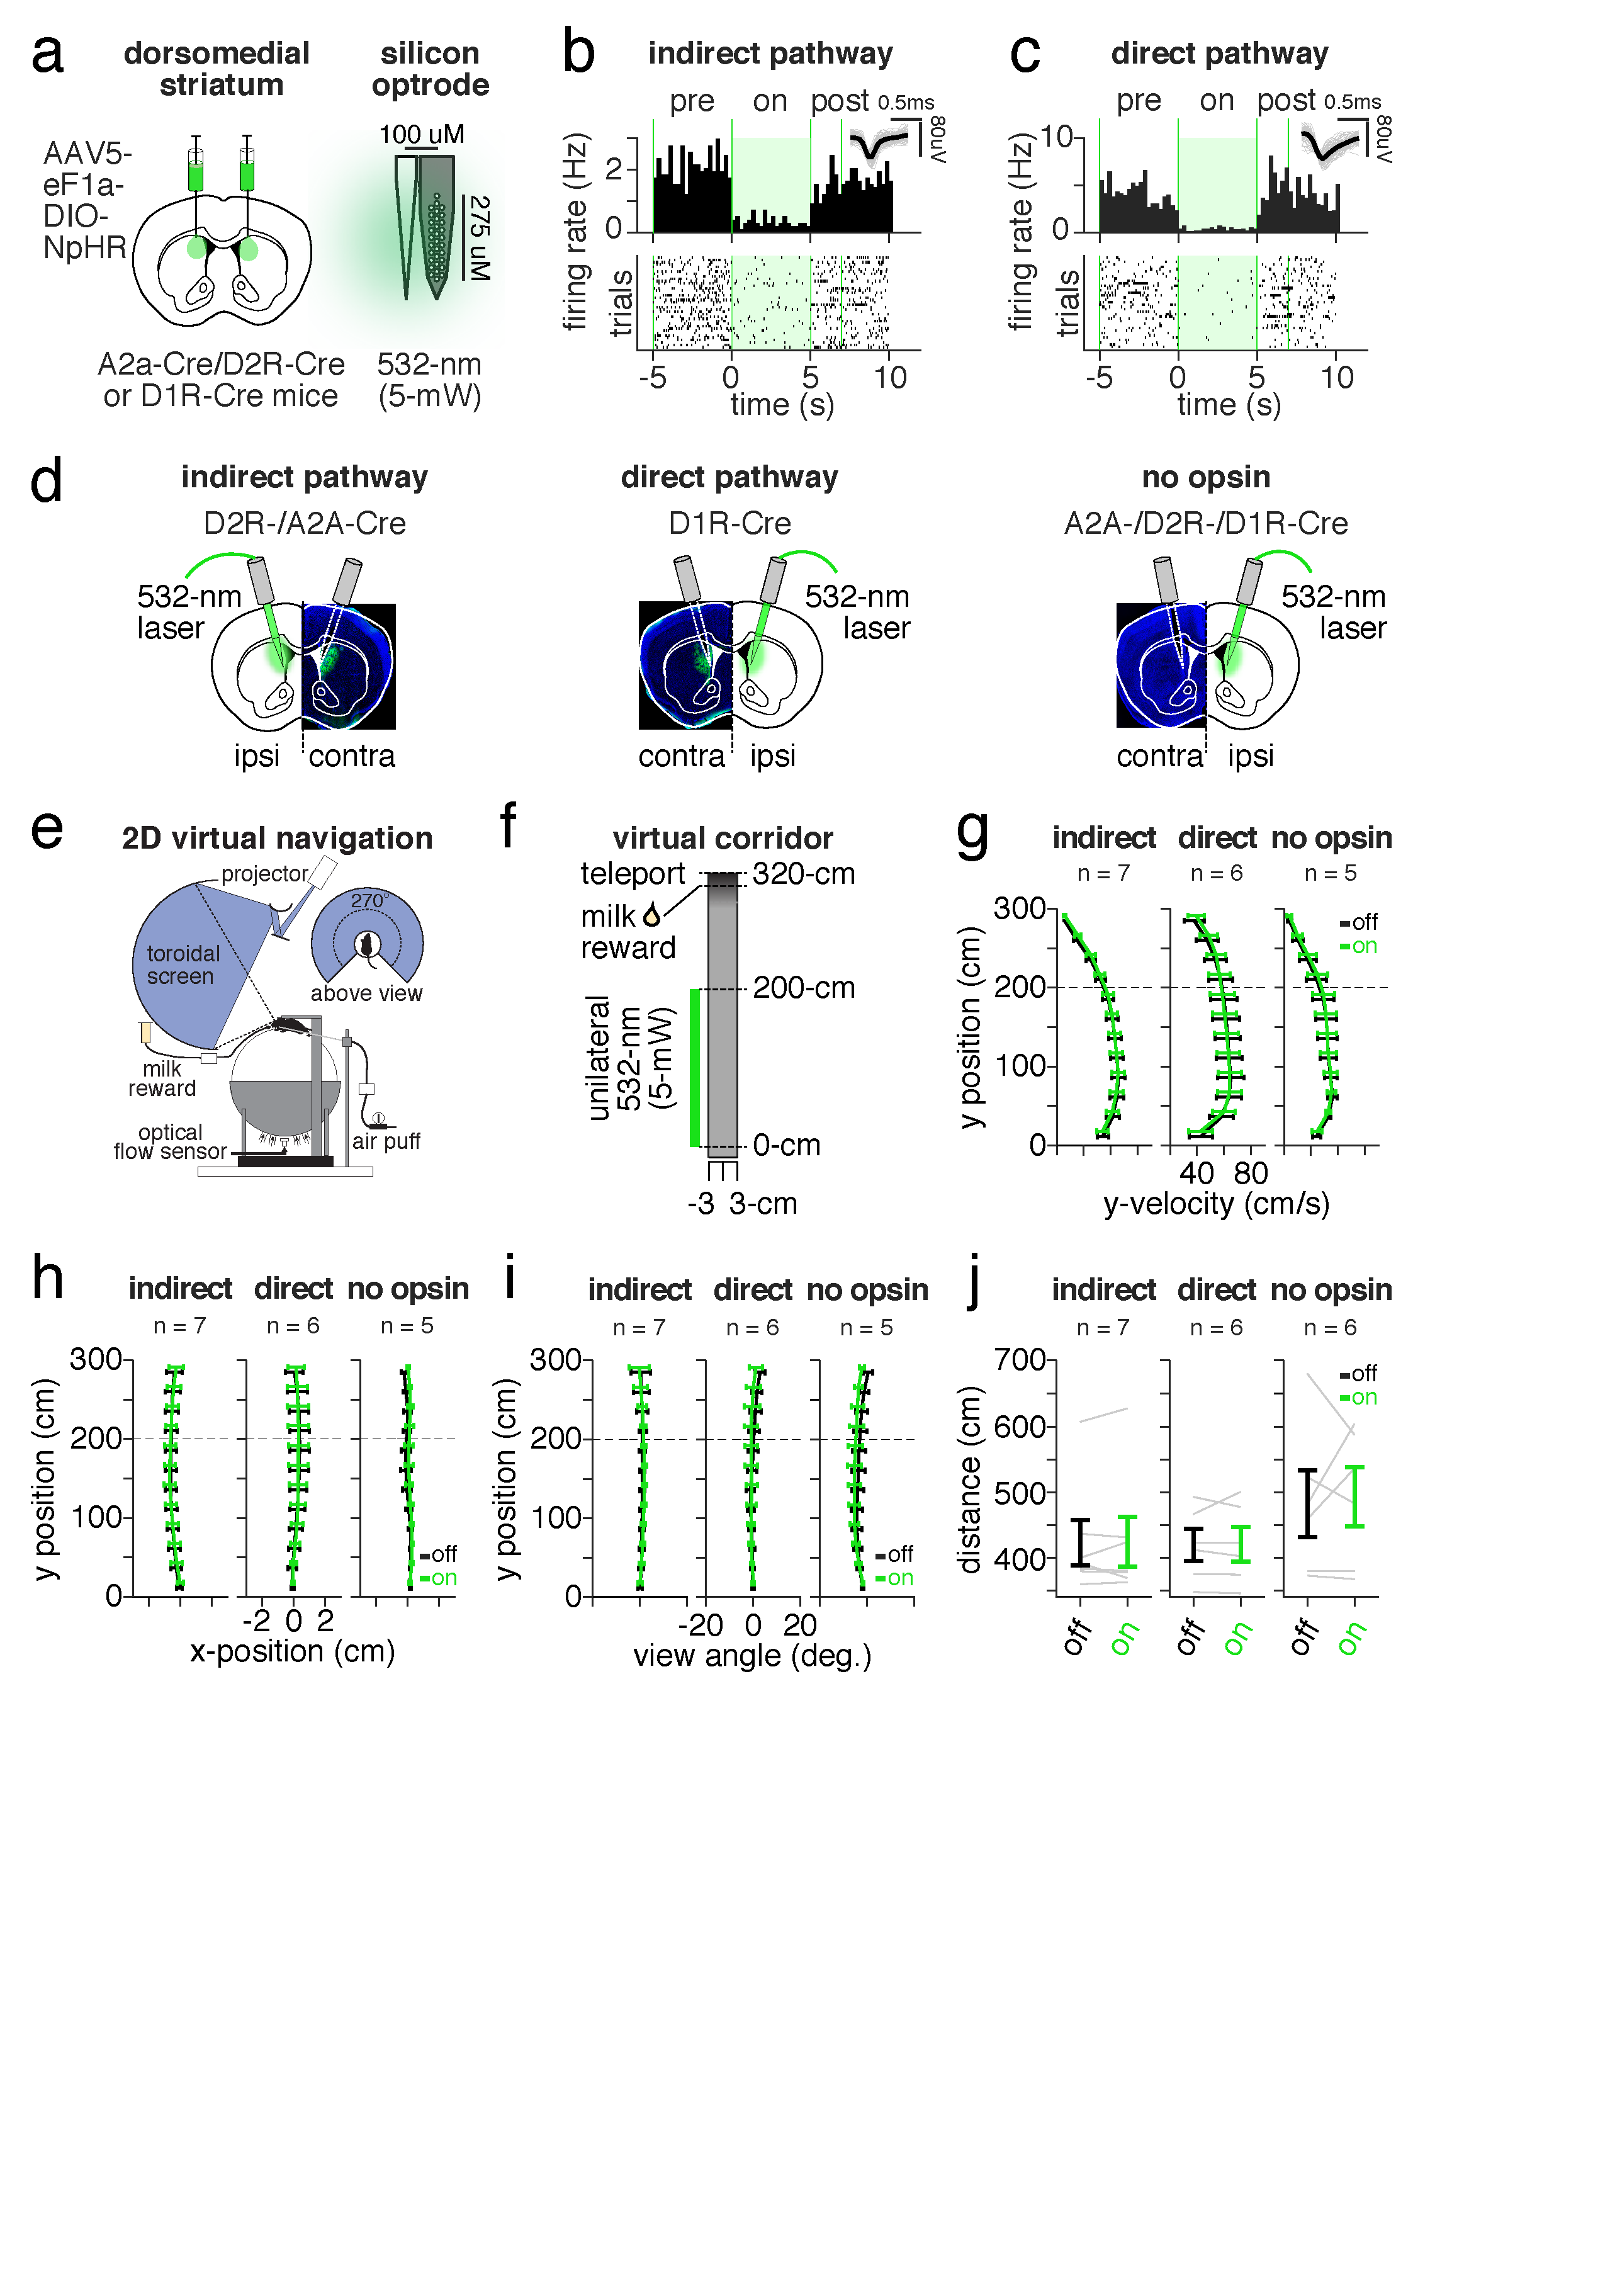
\includegraphics[width=0.90\linewidth]{ch2-glmhmm/glmhmm-figures/Fig1.pdf}
    \caption[Pathway-specific DMS inhibition has no detectable impact on movement in mice navigating a virtual corridor]{\textbf{Pathway-specific DMS inhibition has no detectable impact on movement in mice navigating a virtual corridor.} (a) Schematic of viral delivery of Cre-dependent halorhodopsin (NpHR) to the dorsomedial striatum (DMS) of A2a-Cre, D2R-Cre, or D1R-Cre mice (left). Schematic of optrode (right): a 32-channel silicon probe coupled with tapered optical fiber, which delivered 532-nm (5-mW) light to the DMS of awake, ambulating mice. (b) Example peristimulus time histograms (PSTH) (top) and rasters of trial-by-trial spike times (bottom) from a DMS single-unit recorded in an ambulating A2a-Cre mouse expressing Cre-dependent NpHR (indirect pathway). Inset: average spike waveform (black) and 100 randomly sampled spike waveforms (grey). A trial consisted of 5-s without laser (pre, -5 to 0-s), 5-s laser sweep (on, 0 to 5-s), and 10-s ITI (40 total trials). (c) As in b but for DMS single-unit in a D1R-Cre mouse expressing}
    \label{fig:glmhmm:1}
  \end{center}
  \vspace{-1.5cm}
\end{figure}
\begin{figure}[t!]
  \contcaption{Cre-dependent NpHR (direct pathway). (d) Schematic of bilateral fiberoptic implantation of DMS and unilateral illumination in behaving mice, with example histology from a mouse expressing NpHR in the indirect (left, D2R-/A2a-Cre) or direct (middle, D1R-Cre) pathways, or control mouse without opsin (right, no opsin, A2a-/D2R- or D1R-Cre). 532-nm light (5-mW) was delivered unilaterally to the left or right hemisphere on alternate testing sessions and lateralized behavior was defined as ipsilateral or contralateral relative to the laser hemisphere. (e) Schematic of head-fixation of mice in a virtual reality (VR) apparatus allowing 2-D navigation. Displacements of an air-suspended spherical ball in the anterior-posterior (and medial-lateral) axes of the mouse controlled y- (and x-) position movements in a visual VR environment. (f) Schematic of virtual corridor 6-cm in width and 330-cm in length, consisting of a start region (-10-0cm), an inhibition region (0-200cm) in which mice received unilateral 532-nm light on a random subset of trials (30\%), a reward location (310cm) where mice received reward, and a teleportation location (320cm) where mice were transported to the start region following a variable ITI with mean of 2-s. (g) Average y-velocity (cm/s) across mice as a function of y-position (0-300cm in 25-cm bins) while navigating the virtual corridor on laser off (black) or laser on (green) trials in groups receiving DMS indirect (left, n = 7 mice, n = 1,712 laser off and n = 1,288 laser on trials) or direct pathway inhibition (middle, n = 6 mice, n = 1,088 laser off and n = 757 laser on trials), or illumination of the DMS in the absence of NpHR expression (right, no opsin, n = 5 mice, n = 1,178 laser off and n = 827 laser on trials). (h) Same as g but for average x-position (cm) contralateral to the unilaterally-coupled laser hemisphere. (i) Same as g but for view angle (degrees, contralateral to laser hemisphere). (j) Average across-mouse distance travelled (cm) to traverse the virtual corridor during laser off (black) or laser on (green) trials for mice receiving DMS indirect (n = 7 mice, n = 2,109 laser off and n = 1,574 laser on trials) or direct pathway inhibition (n = 6 mice, n = 1,330 laser off and n = 930 laser on trials), or DMS illumination in the absence of NpHR (n = 6  mice, n = 1,688 laser off and n = 1,199 laser on trials). Solid bars depict mean +/-S.E.M. across mice; grey lines indicate individual mouse mean.}% Continued caption
\end{figure}

To determine if endogenous activity in DMS pathways provides bidirectional control of motor output in the absence of a decision, we carried out unilateral inhibition of indirect and direct pathways in head-fixed mice running on an air-supported ball to traverse a 2-dimensional linear corridor in virtual reality (VR) (Fig. 1d-f, 6-cm x 330-cm corridor). Illumination of the DMS was restricted to 0-200cm (laser on 30\% of trials; hemisphere of illumination alternated across days). The parameters of the virtual corridor and inhibition period were selected to closely match the stem of the VR-based T-maze decision-making tasks that are the focus of subsequent experiments.

We found no detectable impact of pathway-specific DMS inhibition, nor DMS illumination alone, on multiple indicators of motor output during virtual corridor navigation. This included measures of velocity, x-position or view angle relative to the laser hemisphere, and distance traveled (Fig. 1g-j; see Extended Data Fig. 2 for additional measures). Similarly, we obtained null effects of pathway-specific inhibition on velocity (and spatial preference) in freely behaving mice in a conditioned place preference assay (Supplementary Fig. 3). 

These negative findings argue against a major involvement of endogenous activity in DMS pathways in the execution of movement in the absence of a decision. This is consistent with the dearth of reports demonstrating strong and opposing modulation of behavior by striatal pathways using pathway-specific optogenetic inhibition. 

\subsection{Three virtual reality T-mazes with varying cognitive demands}
\label{sec:glmhmm:2.2.3}
We next considered the possibility that, rather than contributing directly to a motor output, endogenous activity in DMS pathways may instead have opposing influence over decisions in a manner that is dependent on cognitive demand. To test this idea, we trained mice to perform a set of VR-based, decision-making tasks \cite{pinto_accumulation--evidence_2018} that shared identical motor readouts (left or right choice), had highly similar sensory environments, and yet differed in their cognitive requirements (Fig. \ref{fig:glmhmm:2}a,b).

The first task was an ‘evidence accumulation’ task, in which visuo-tactile cues were transiently presented on each side of the central stem of a virtual T-maze according to a Poisson distribution (‘cue region’, 0–200cm), and mice were rewarded for turning to the maze side with the greater number of cues (Fig. \ref{fig:glmhmm:2}a,b; black). Thus, mice were required to continually accumulate sensory cues over several seconds into a memory (or motor plan) that guided their left/right decision.

In two additional control tasks, we made modifications intended to weaken the cognitive demands of each task. In the first control task (‘no distractors’), cues were presented on the rewarded maze side during the same maze region (0–200cm) according to the same Poisson distribution, but distractor cues on the side of the non-rewarded arm were omitted (Fig. \ref{fig:glmhmm:2}a,b; magenta). The absence of distractors on the non-rewarded side meant that each cue signaled reward with 100\% probability, and thus gradual evidence accumulation was not required. Further ensuring that evidence accumulation was not required, an additional cue at the end of the maze was present only during the cue period (0–200cm) to signal the rewarded side.

\begin{figure}[t!]
  \begin{center}
    \includegraphics[width=0.90\linewidth]{ch2-glmhmm/glmhmm-figures/Fig2.pdf}
    \caption[A set of virtual reality T-mazes have similar sensory features and identical motor requirements but different cognitive demands]{\textbf{A set of virtual reality T-mazes have similar sensory features and identical motor requirements but different cognitive demands.} (a) Schematic of three virtual reality (VR)-based T-maze tasks. (b) Example mouse perspective  at the same maze position (-10cm, 120cm, 195cm, and 295cm) from the example trial depicted in a of the evidence accumulation (left, black), no distractors (middle, ctrl 1), or permanent cues (right, ctrl 2) tasks. (c) Average choice accuracy (\% correct) across mice performing the accumulation of evidence (black, n = 32 mice, n = 52,381 trials), no distractors (magenta, ctrl 1: n = 31 mice, n = 56,783 trials), or permanent cues (cyan, ctrl 2: n = 20 mice, n = 27,870 trials) tasks. p-value denotes one-way ANOVA of task on accuracy (p = 1.3 x 10-23, F2,80 = 109.4). Asterisks indicate statistical significance of post-hoc, unpaired, two-tailed ranksum comparisons of accuracy between groups (top to bottom: ***p = 3.9 x 10-7, z = -5.1; ***p = 2.1 x 10-11, z = -6.7; ***p = 2.1 x 10-5, z = 4.3). (d) Average y-velocity (cm/s) across mice as a function of y-position (0-300 cm in 25cm bins) during performance of each task (colors and n as in c). (e) Same as d but for average x-position (cm) on left and right choice trials. (f) Same as d but for average view angle (degrees) on left and right choice trials. (g) Average distance (cm) traveled per trial across mice (evidence accumulation, n = 32 mice, n = 53,833 trials; no distractors (control 1): n = 32 mice, n = 60,074 trials; permanent cues (control 2): n = 20 mice, n = 29,192 trials). p-value reflects one-way ANOVA of task on distance (p = 0.16, F2,81 = 1.8). Throughout solid bars denote across mouse mean values $\pm$S.E.M. and transparent ‘x’ indicate individual mouse mean.}
    \label{fig:glmhmm:2}
  \end{center}
  \vspace{-0.5cm}
\end{figure}

In the second control task (‘permanent cues’), the sensory statistics of the cues were identical to those in the evidence accumulation task, but rather than transient visual cue presentation, visual cues were permanently visible from trial onset (Fig. \ref{fig:glmhmm:2}a,b; cyan). This maintained the same conceptual task structure of the evidence accumulation task while decreasing the memory demands, as the sensory cues (or the motor plan) did not need to be remembered until the cues were passed.

We assessed how task demands impacted choice accuracy in each task. Consistent with the greatest cognitive and mnemonic demand in the evidence accumulation task, we found that overall choice accuracy was significantly lower compared to both control tasks (Fig. \ref{fig:glmhmm:2}c, AoE: 73.1 $\pm$ 0.8\%. Ctrl 1: 90.6 $\pm$ 0.9\%. Ctrl 2: 83.3 $\pm$ 1.2\% mean $\pm$ s.e.m).

While the motor requirements of a decision were the same across tasks (crossing an x-position threshold at the end of the central stem; Methods), we examined the possibility that cross-task differences in cognitive requirements altered movement within the stem of the maze (0–300cm). We observed no consistent cross-task differences in velocity, x-position or view angle on left or right choice trials, nor distance traveled (Fig. \ref{fig:glmhmm:2}d–g; see Extended Data Fig. \ref{fig:ap1:ext3}a–f for additional measures). We further compared the relationship between behavior in the stem of the maze and choice across tasks by using a decoder to predict choice based on the trial-by-trial x-position or view angle (Extended Data Fig. \ref{fig:ap1:ext3}g–j) at successive maze positions (0–300cm in 25-cm bins). While we were able to predict choice from either measure above chance levels in all three tasks (consistent with previous studies \cite{pinto_accumulation--evidence_2018}), choice prediction accuracy was statistically indistinguishable across tasks (Extended Data Fig. \ref{fig:ap1:ext3}g–j). Together, this indicated that cross-task differences in task demands did not prompt mice to systematically adopt distinct motor strategies.
\subsection{Behavioral effects of dorsomedial striatum pathway inhibition depend on task demand}
\label{sec:glmhmm:2.2.4}
We performed unilateral inhibition of DMS indirect and direct pathways restricted to the cue region (0–200cm) of each task (Fig. 3a,b; laser on 10–20\% of trials; hemisphere of illumination alternated across days). We found that inhibition of the indirect pathway produced a large bias toward contralateral choices during the accumulation of evidence task (Fig. 3c,d), which was significantly greater than that observed in control animals that did not express opsin (Fig. 3e, average contralateral bias: DMS indirect, 42.3\%$\pm$4.4\%, versus no opsin, 5.9\%$\pm$.6\%). Similarly, inhibition of the direct pathway also produced a large choice bias during the accumulation of evidence task (Fig. 3d; average contralateral bias: DMS direct, -36.8\%$\pm$8.6\%), which was also significantly greater than that observed in control animals (Fig. 3e). However, in this case, the direction of the choice bias was in the opposite (ipsilateral) direction to that observed with indirect pathway inhibition (also see Extended Data Fig. \ref{fig:ap1:ext4}a–i for psychometric curves).

Providing a stark contrast to the large effects of pathway-specific DMS inhibition on choice during the evidence accumulation task, inhibition of either pathway had significantly less impact on choice during the ‘no distractors’ and ‘permanent cues’ control tasks (Fig. \ref{fig:glmhmm:3}f–k and Extended Data Fig. \ref{fig:ap1:ext5}a–c; unpaired, two-tailed Wilcoxon rank-sum test of indirect pathway inhibition evidence accumulation versus no distractors, $P=8.0 \times 10^{-4}$, z=3.4, or evidence accumulation versus permanent cues, $P=0.001$, $z=3.3$; and direct pathway inhibition evidence accumulation versus no distractors, $P=0.002$, $z=-3.1$, or evidence accumulation versus permanent cues, $P=0.005$, $z=-2.8$). In fact, the effects of pathway-specific DMS inhibition on choice bias in either control task did not significantly differ from those observed in control animals (Fig. 3h, for ‘no distractors’; Fig. \ref{fig:glmhmm:3}k, for ‘permanent cues’; see also Extended Data Fig. \ref{fig:ap1:ext4}a–i for psychometric curves).

Thus, inhibition of DMS pathways elicited strong and opposing effects on choice in the task with the greatest cognitive demand, which required the accumulation of sensory evidence across multiple seconds to arrive at a decision and had a far limited impact on choice in task variants with reduced cognitive demand.

\begin{figure}[t!]
  \begin{center}
    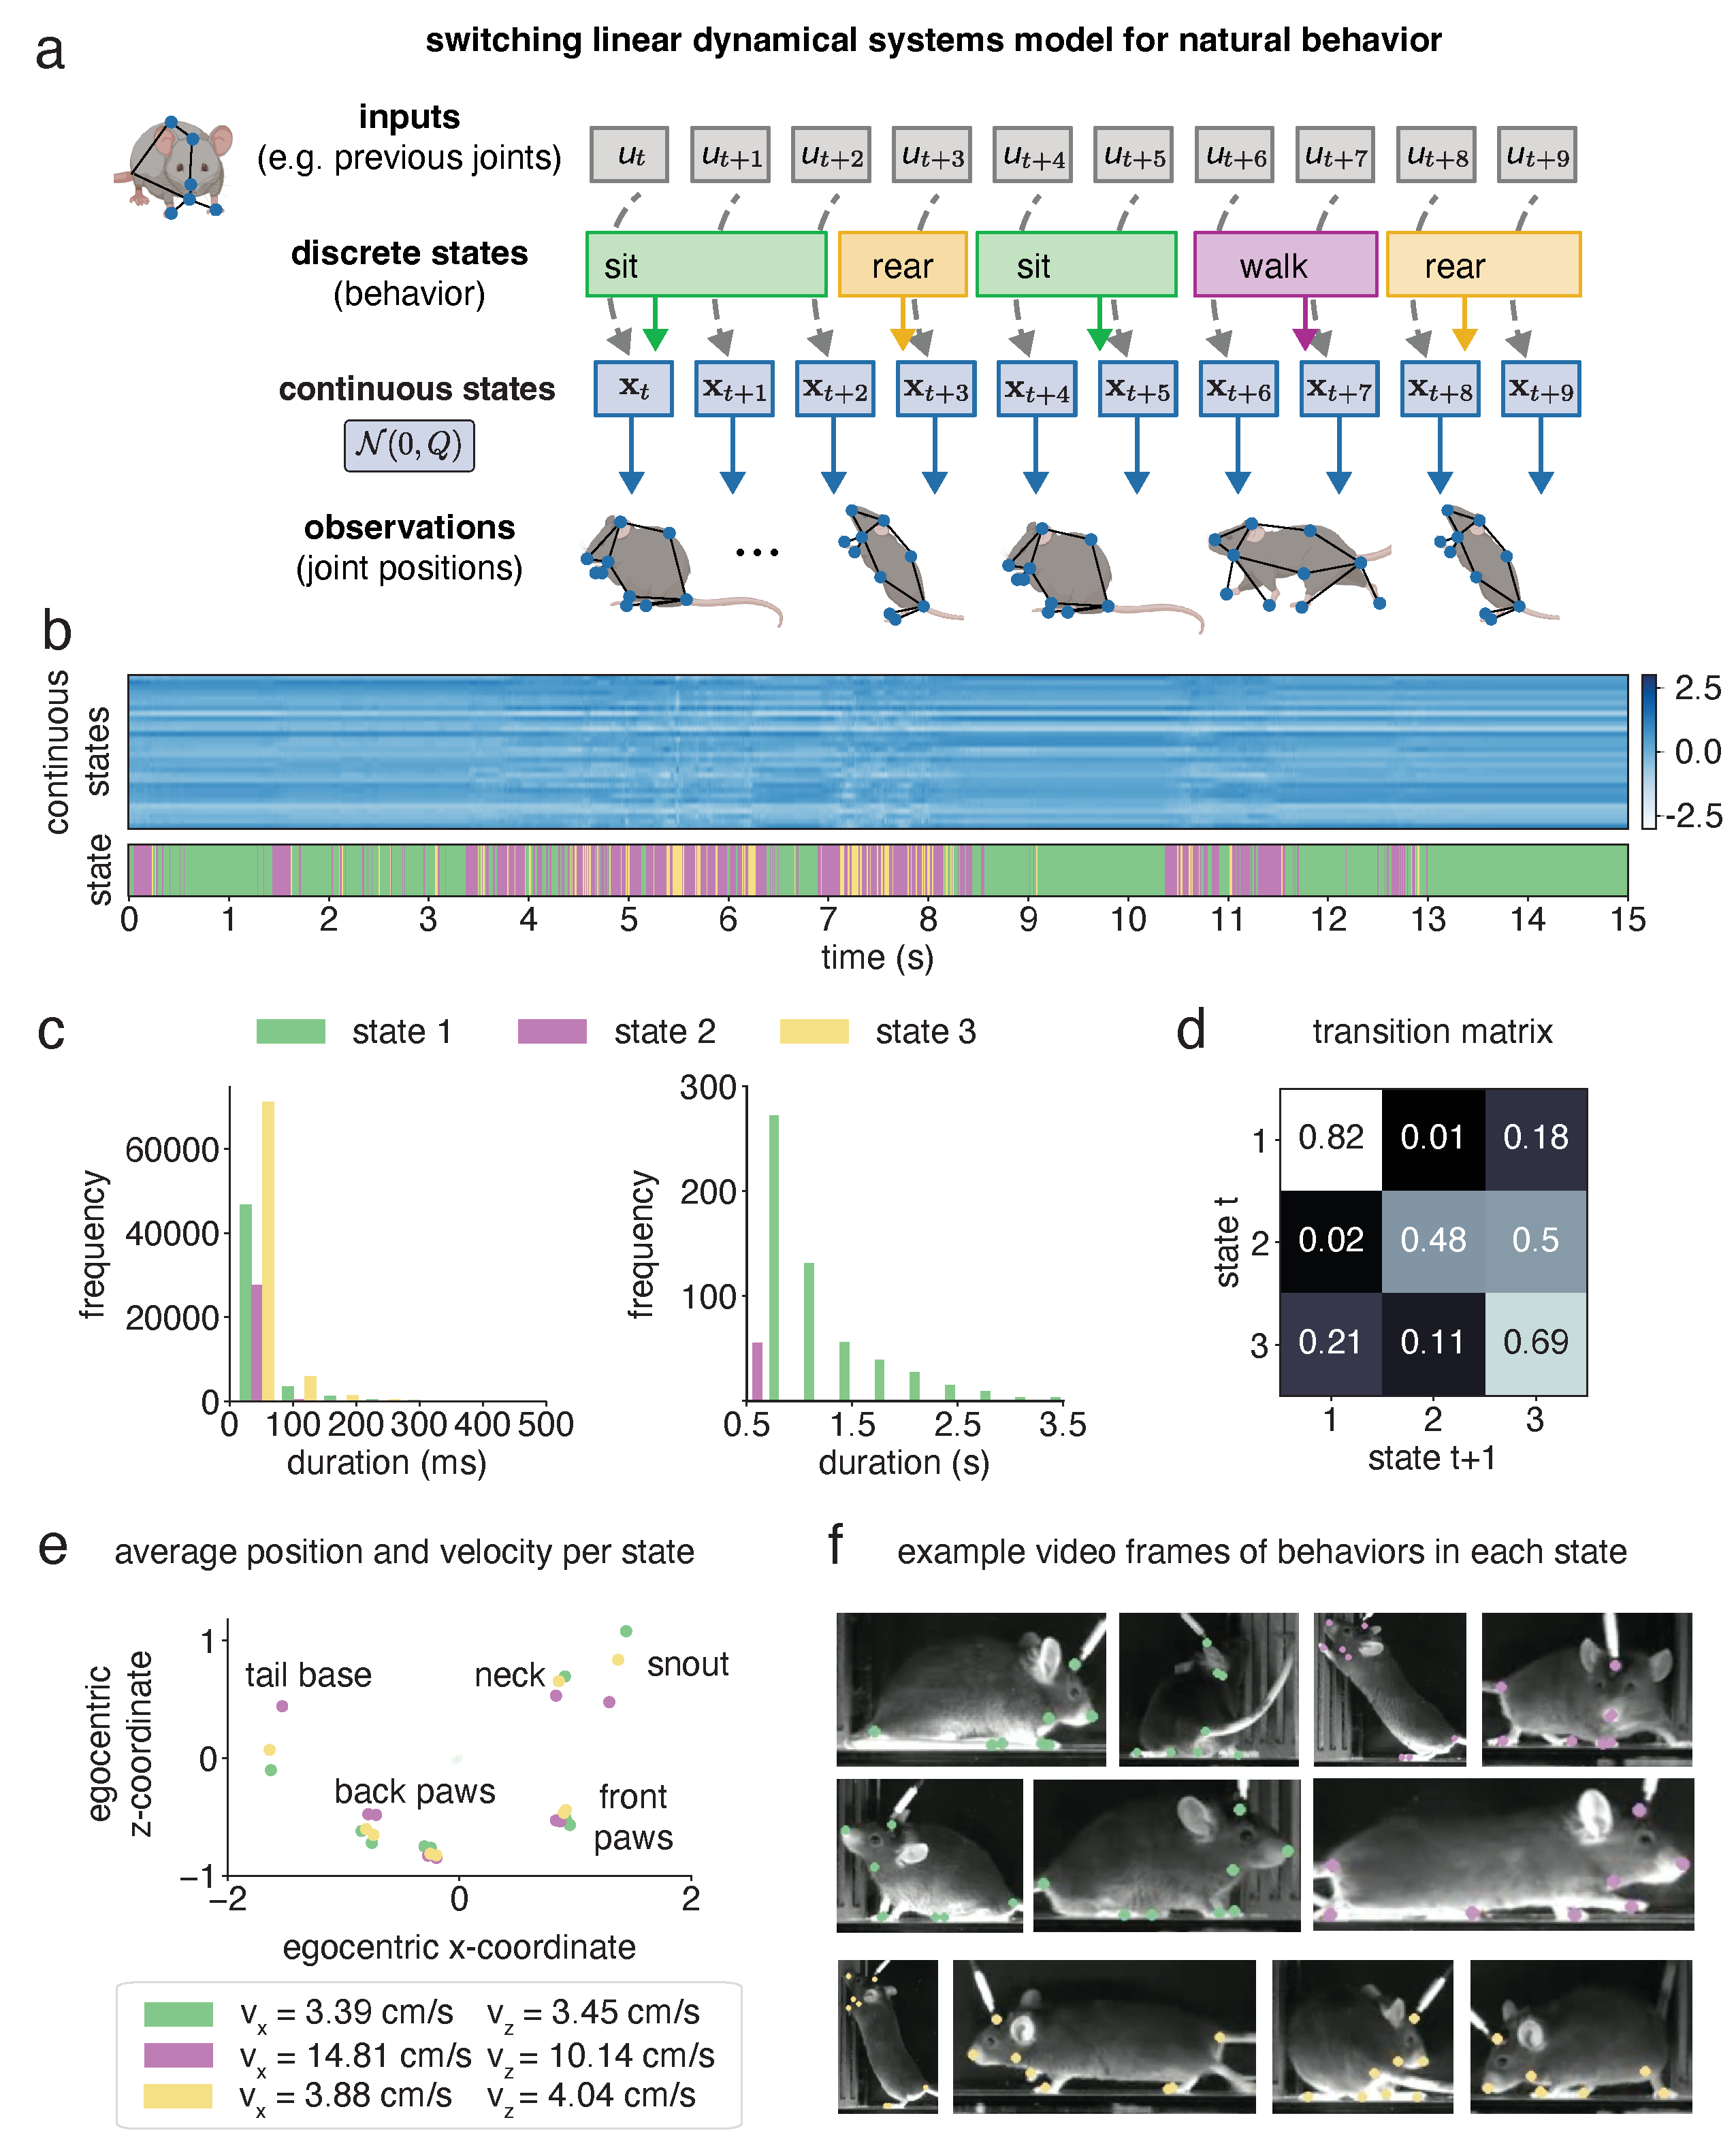
\includegraphics[width=0.90\linewidth]{ch2-glmhmm/glmhmm-figures/Fig3.pdf}
    \caption[Inhibition of DMS but not NAc pathways has strong and opposing influence on choice during an evidence accumulation task, while having weaker effects during task variants with diminished cognitive demands]{\textbf{Inhibition of DMS but not NAc pathways has strong and opposing influence on choice during an evidence accumulation task, while having weaker effects during task variants with diminished cognitive demands.} }
    \label{fig:glmhmm:3}
  \end{center}
  \vspace{-1.5cm}
\end{figure}
\begin{figure}[t!]
  \contcaption{(a) Schematic of bilateral viral delivery of Cre-dependent NpHR to the dorsomedial striatum (DMS). (b) Schematic of bilateral fiberoptic implantation of the DMS and unilateral inhibition in behaving mice, with example histology from a mouse expressing NpHR in the indirect (left, D2R-/A2a-Cre) or direct (middle, D1R-Cre) pathways, or DMS illumination in the absence of NpHR (right, no opsin, A2a-/D2R- or D1R-Cre). 532-nm light (5-mW) was delivered unilaterally to the left or right hemisphere on alternate testing sessions and choice bias contralateral or ipsilateral to the hemisphere of inhibition was quantified. (c) Schematic of the evidence accumulation task with delivery of 532-nm light restricted to the cue region (0-200cm) on a random subset of trials (10-20\%). (d) Average across mouse choice bias during the evidence accumulation task. Choice bias was defined as the difference between percent correct performance on trials when the correct choice was contralateral or ipsilateral to the inhibited hemisphere (\% correct, contralateral-ipsilateral, positive values indicate a contralateral bias). Bias was calculated separately on laser off (black) and laser on (green) trials for mice receiving unilateral indirect pathway inhibition (left, n = 11 mice, n = 16,935 laser off and n = 3,390 laser on trials), unilateral direct pathway inhibition  (middle: n = 10 mice; n = 14,030 laser off and n = 3,103 laser on trials), or unilateral illumination of the DMS in the absence of NpHR (right, n = 11 mice, n = 21,422 laser off and n = 5,113 laser on trials). (e) Difference in contralateral choice bias (\% correct, contralateral-ipsilateral) between laser off and on trials (\% bias, on-off) in mice performing the evidence accumulation task and receiving indirect pathway inhibition, direct pathway inhibition, or DMS illumination in the absence of NpHR. Asterisks indicate significance of unpaired, two-tailed Wilcoxon ranksum comparison of indirect to no opsin: ***p = 1.1x10-4, z = 3.9; direct to no opsin: ***p = 2.2x10-4, z = -3.7). (f-h) Same as c-e but for the no distractors (control 1) task. Indirect: n = 7 mice, n = 13,706 laser off and n = 3,288 laser on trials; direct: n = 9 mice, n = 14,647 laser off and n = 3,682 laser on trials; no opsin: n = 4 mice, n = 3,654 laser off and n = 901 laser on trials. Asterisks indicate significance of unpaired, two-tailed Wilcoxon ranksum comparison of indirect to no opsin: not significant (n.s.), p = 0.22, z = 1.2. Direct to no opsin: not significant (n.s.), p = 0.08, z = -1.8. (i-k) As in c-e but for the permanent cues (control 2) task. Indirect: n = 7 mice, n = 4,033 laser off and n = 929 laser on trials; direct: n = 7 mice, n = 6,061 laser off and n = 1,494 laser on trials; no opsin: n = 6 mice, n = 3,975 laser off and n = 923 laser on trials. Asterisks indicate significance of unpaired, two-tailed Wilcoxon ranksum comparison of indirect to no opsin: not significant (n.s.), p = 0.13, z = 1.5. Direct to no opsin: not significant (n.s.), p = 0.62, z = 0.5. (l) As in a but for bilateral viral delivery of Cre-dependent NpHR to the nucleus accumbens (NAc). (m) Same as b but for bilateral fiberoptic implantation of the NAc and unilateral inhibition in behaving mice, with example histology from a mouse expressing NpHR in the indirect (left, D2R-/A2a-Cre) or direct (middle, D1R-Cre) pathways, or NAc illumination in the absence of NpHR (right, no opsin, A2a-/D2R- or D1R-Cre). (n-p) As in c but for pathway-specific NAc inhibition during the accumulation of evidence task. Indirect: n = 9 mice, n = 11,978 laser off and n = 2,604 laser on trials; direct: n = 10 mice, n = 15,430 laser off and n = 3,348 laser on trials; no opsin: n = 7 mice, n = 9,819 laser off and n = 1,488 laser on trials. Asterisks indicate significance of unpaired, two-tailed Wilcoxon ranksum comparison of indirect to no opsin: not significant (n.s.), p = 0.86, z = 0.18; direct to no opsin: not significant (n.s.), p = 0.04, z = 2.0. Throughout solid bars denote across mouse mean values $\pm$S.E.M. and transparent ‘x’ indicate individual mouse mean. To account for multiple group comparisons we considered p-values significant after Bonferroni correction (2 comparisons).}% Continued caption
\end{figure}

While DMS pathway inhibition had minimal impact on movement in a virtual corridor (Fig. \ref{fig:glmhmm:1} and Extended Data Fig. \ref{fig:ap1:ext2}), we considered the possibility that pathway-specific DMS inhibition altered motor performance in the T-mazes. We found no cross-task differences in the effects of pathway-specific inhibition on measures of velocity, distance traveled or per-trial standard deviation in view angle (Extended Data Fig. \ref{fig:ap1:ext6}a–i). However, we found subtle but opposing effects of pathway-specific inhibition on average x-position and view angle (Extended Data Fig. \ref{fig:ap1:ext6}j–k) in the evidence accumulation task. The direction of these biases was similar in the control tasks, but consistently smaller than in the evidence accumulation task. Thus, in line with the close relationship between x-position/view angle and choice in the absence of inhibition in each task (Extended Data Fig. \ref{fig:ap1:ext3}g–j), pathway-specific DMS inhibition produced the same general pattern of cross-task effects on choice bias (Extended Data Fig. \ref{fig:ap1:ext5}b–d) and x-position/view angle (Extended Data Fig. \ref{fig:ap1:ext6}j,k). As the quantitative relationship between x-position or view angle and choice is indistinguishable across tasks in the absence of neural inhibition (Extended Data Fig. \ref{fig:ap1:ext3}g–j), cross-task differences in motor strategy do not provide a trivial explanation for these effects. Rather, taken together with the absence of an effect of pathway-specific DMS inhibition on motor output in the virtual corridor (Fig. \ref{fig:glmhmm:1}h,i), these data imply that the effects of inhibition on behavior depend on cognitive demands.
\subsection{Little effect of nucleus accumbens pathway inhibition on choice}
\label{sec:glmhmm:2.2.5}

We next sought to determine whether opponent control of choice by striatal pathways during the evidence accumulation task was specific to the DMS, or if it extended to the ventral striatum. To this end, we delivered unilateral laser illumination to the nucleus accumbens (NAc) of mice expressing NpHR in the indirect or direct pathways (or non-opsin control mice), which was restricted to the cue region (0–200cm) of the evidence accumulation task (Fig. \ref{fig:glmhmm:3}l–p and Extended Data Fig. \ref{fig:ap1:ext4}j–l).

Providing a clear functional dissociation between DMS and NAc, effects of pathway-specific NAc inhibition on choice bias were significantly smaller than those observed with inhibition of DMS pathways (Extended Data Fig. \ref{fig:ap1:ext5}e,f; unpaired, two-tailed Wilcoxon rank-sum test of DMS versus NAc indirect pathway inhibition, $P=2.6 \times 10^{-4}$, $z=3.6$; of DMS versus NAc direct pathway inhibition, $P=1.8 \times 10^{-4}$, $z=-3.7$), and were also not significantly different from NAc control animals (Fig. \ref{fig:glmhmm:3}o,p). It is unlikely that this dissociation between DMS and NAc can be explained by greater coexpression of pathway-specific markers in the ventral versus dorsal striatum \cite{kupchik_coding_2015}, as both subregions exhibited equally low colocalization of D1R and D2R receptors (Supplementary Fig. \ref{fig:ap1:supp1}j–l).
\subsection{Bernoulli generalized linear model does not fully capture psychometric curves}
\label{sec:glmhmm:2.2.6}

Our inactivation experiments suggest that DMS pathways make strong contributions to behavior during a cognitively demanding evidence accumulation task, but do not contribute strongly to similar tasks with weaker cognitive demands. However, even during the evidence accumulation task, it is possible that the animals’ level of cognitive engagement varies over time. This raises the possibility that the contributions of the two pathways to behavior could change over time, even within the same task.

To address this possibility, we sought to understand the factors that contribute to decisions in the evidence accumulation task. As a first step, we used a Bernoulli generalized linear model (GLM) to predict choice based on a set of external covariates (Fig. \ref{fig:glmhmm:4}a,b). These covariates included the sensory evidence (difference between the number of right and left cues, or ‘$\Delta$ cues’), the recent choice and reward history, the delivery of optical inhibition (‘laser’), as well as a bias. Note that we set the value of the laser covariate to $+1$ (or $-1$) on trials with right (or left) hemisphere inhibition, and zero otherwise. A positive (or negative) GLM weight on this covariate thus captured an ipsilateral (or contralateral) ‘laser’-induced bias in choices relative to the hemisphere of inhibition. For the choice history covariates, a positive weight indicates a tendency toward repeating past choices (\ref{sec:appendix1:methods}).

\begin{figure}[t!]
  \begin{center}
    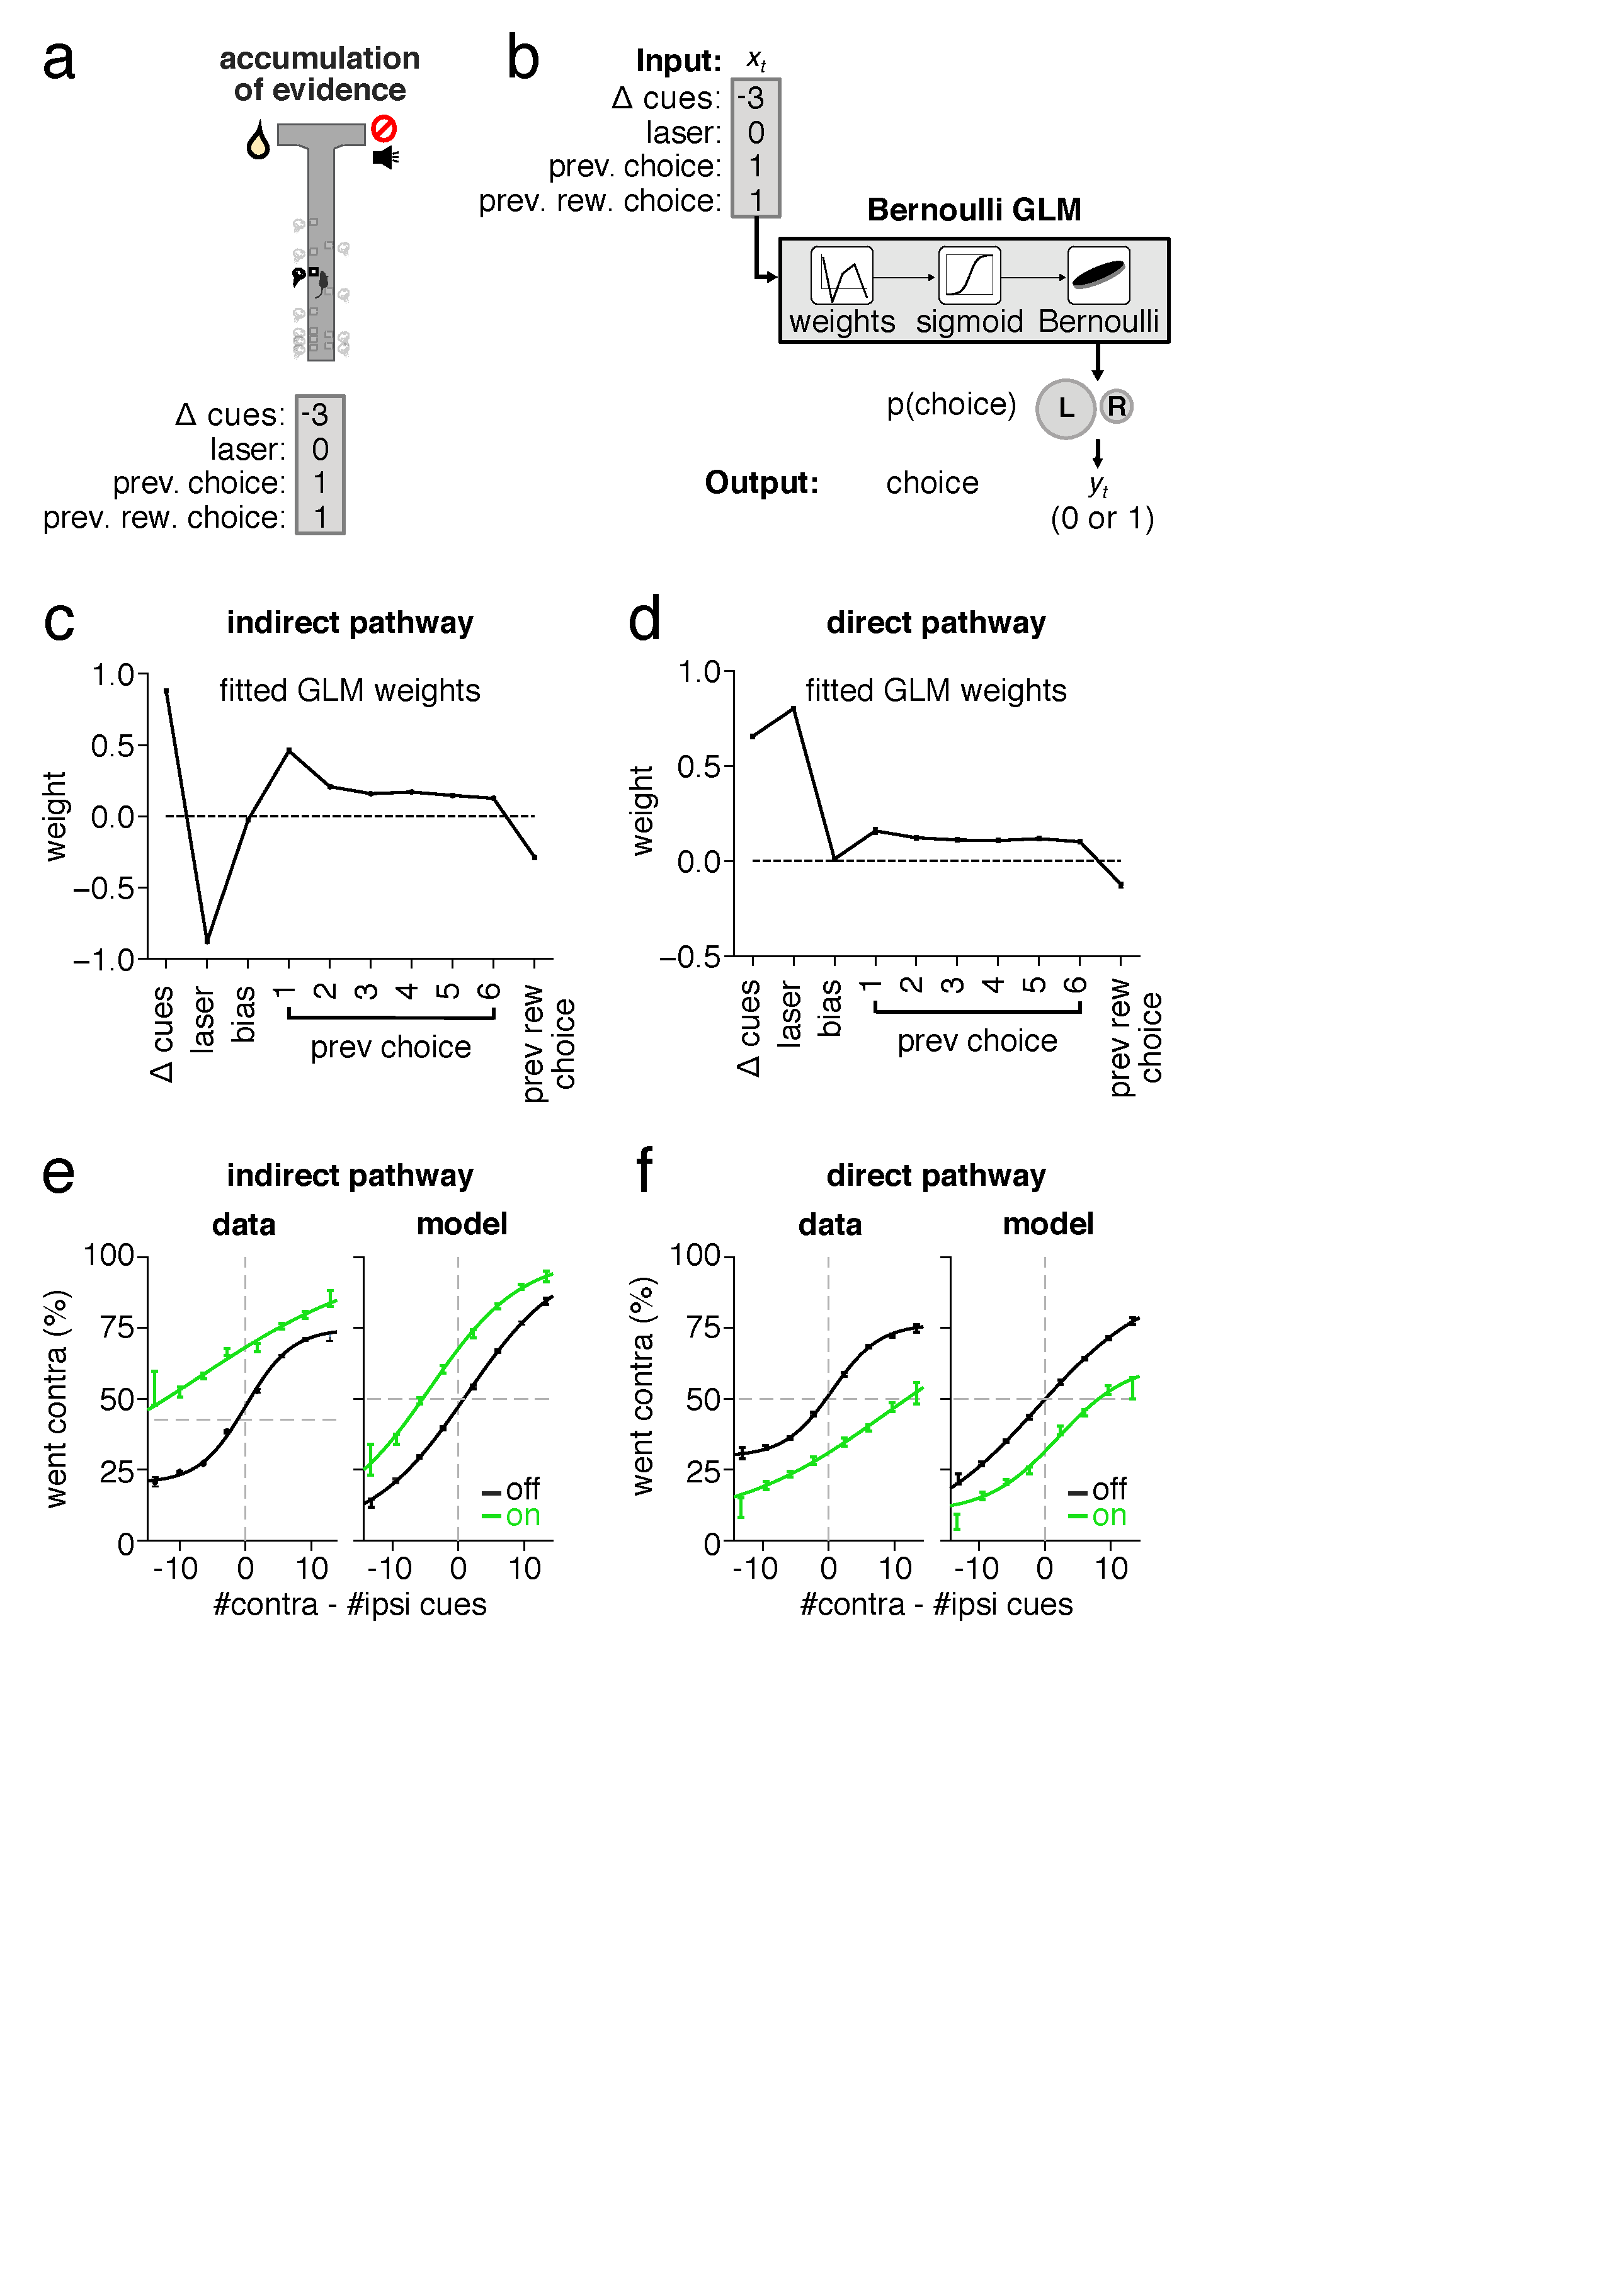
\includegraphics[width=0.70\linewidth]{ch2-glmhmm/glmhmm-figures/Fig4.pdf}
    \caption[A GLM reveals that sensory evidence, dorsomedial striatum pathway inhibition and trial history predict choice during the evidence accumulation task, but does not precisely recapitulate the shape of the psychometric curve.]{\textbf{A GLM reveals that sensory evidence, dorsomedial striatum pathway inhibition and trial history predict choice during the evidence accumulation task, but does not precisely recapitulate the shape of the psychometric curve.} (a) Schematic of the evidence accumulation task and the coding of the external covariates for an example trial.  (b) Schematic of the Bernoulli GLM for an example trial, showing the relationship between external covariates (inputs) and choice on each trial. On each trial, a set of GLM weights maps each input ($\Delta$ cues, laser, bias, previous choice, and existence of a previous rewarded choice) to the probability of each outcome through a sigmoid function, which gives the probability of a “righward” choice on the current trial. (c) Fitted GLM weights using aggregated data from all mice in the indirect pathway DMS inhibition group. The magnitude of each weight indicates the relative importance of that covariate in predicting choice, whereas the sign of the weight indicates the direction of the effect (e.g. a negative laser weight indicates that if inhibition is in the right hemisphere, the mice will be more likely to turn left, while a positive weight on previous choice indicates that if the previous choice was to the right, in the current trial this will bias the mice to turn right again). }
    \label{fig:glmhmm:4}
  \end{center}
  \vspace{-1.5cm}
\end{figure}
\begin{figure}[t!]
  \contcaption{Error bars denote ($\pm$1) posterior standard deviation credible intervals. (d) Same as c but for mice receiving DMS direct pathway inhibition. (e) Fraction of contralateral choice trials as a function of the difference in contralateral versus ipsilateral cues  for laser off (black) and on (green) trials, for mice receiving indirect pathway DMS inhibition for the data (left) and for simulations of the model (right). Error bars denote 95\% confidence intervals around the fraction of choices in each bin of the data; solid curves denote logistic fits (n=13 mice, n = 46,313 laser off and n = 8,570 laser on trials).  (f) Same as e but for the mice receiving direct pathway inhibition of the DMS (n=13 mice, n = 41,250 laser off and n = 7,927 laser on trials).}% Continued caption
\end{figure}

We fit the GLM to aggregated behavioral data from mice inhibited in each DMS pathway and found that sensory evidence, trial history and optical inhibition all contributed to predicting choice (Fig. \ref{fig:glmhmm:4}c,d). As expected, the effect of inhibition of each pathway was large and opposite in sign. However, the GLM did not accurately capture the animals’ psychometric curve, describing the probability of a rightward choice as a function of the sensory evidence (Fig. \ref{fig:glmhmm:4}e,f). This led us to consider variants of the standard GLM that might better account for choice behavior.
\subsection{GLM–HMM better explains choice data with dorsomedial striatum inhibition}
\label{sec:glmhmm:2.2.7}

The standard GLM describes choice as depending on a fixed linear combination of sensory evidence, trial history and the presence or absence of optical inhibition. However, an alternative possibility is that mice use a weighting function that varies over time. To test this idea, we adopted a latent state model with different GLM weights for different states (Fig. \ref{fig:glmhmm:4}). The model consists of a hidden Markov model (HMM) with Bernoulli GLM observations, or GLM–HMM \cite{bengio_input_1994,escola_hidden_2011,calhoun_unsupervised_2019,ashwood_mice_2022} (Fig. 5a,b). Each hidden state is associated with a unique set of GLM weights governing choice behavior in that state. Probabilistic transitions between states occur after every trial, governed by a fixed matrix of transition probabilities (\ref{sec:appendix1:methods}).

\begin{figure}[t!]
  \begin{center}
    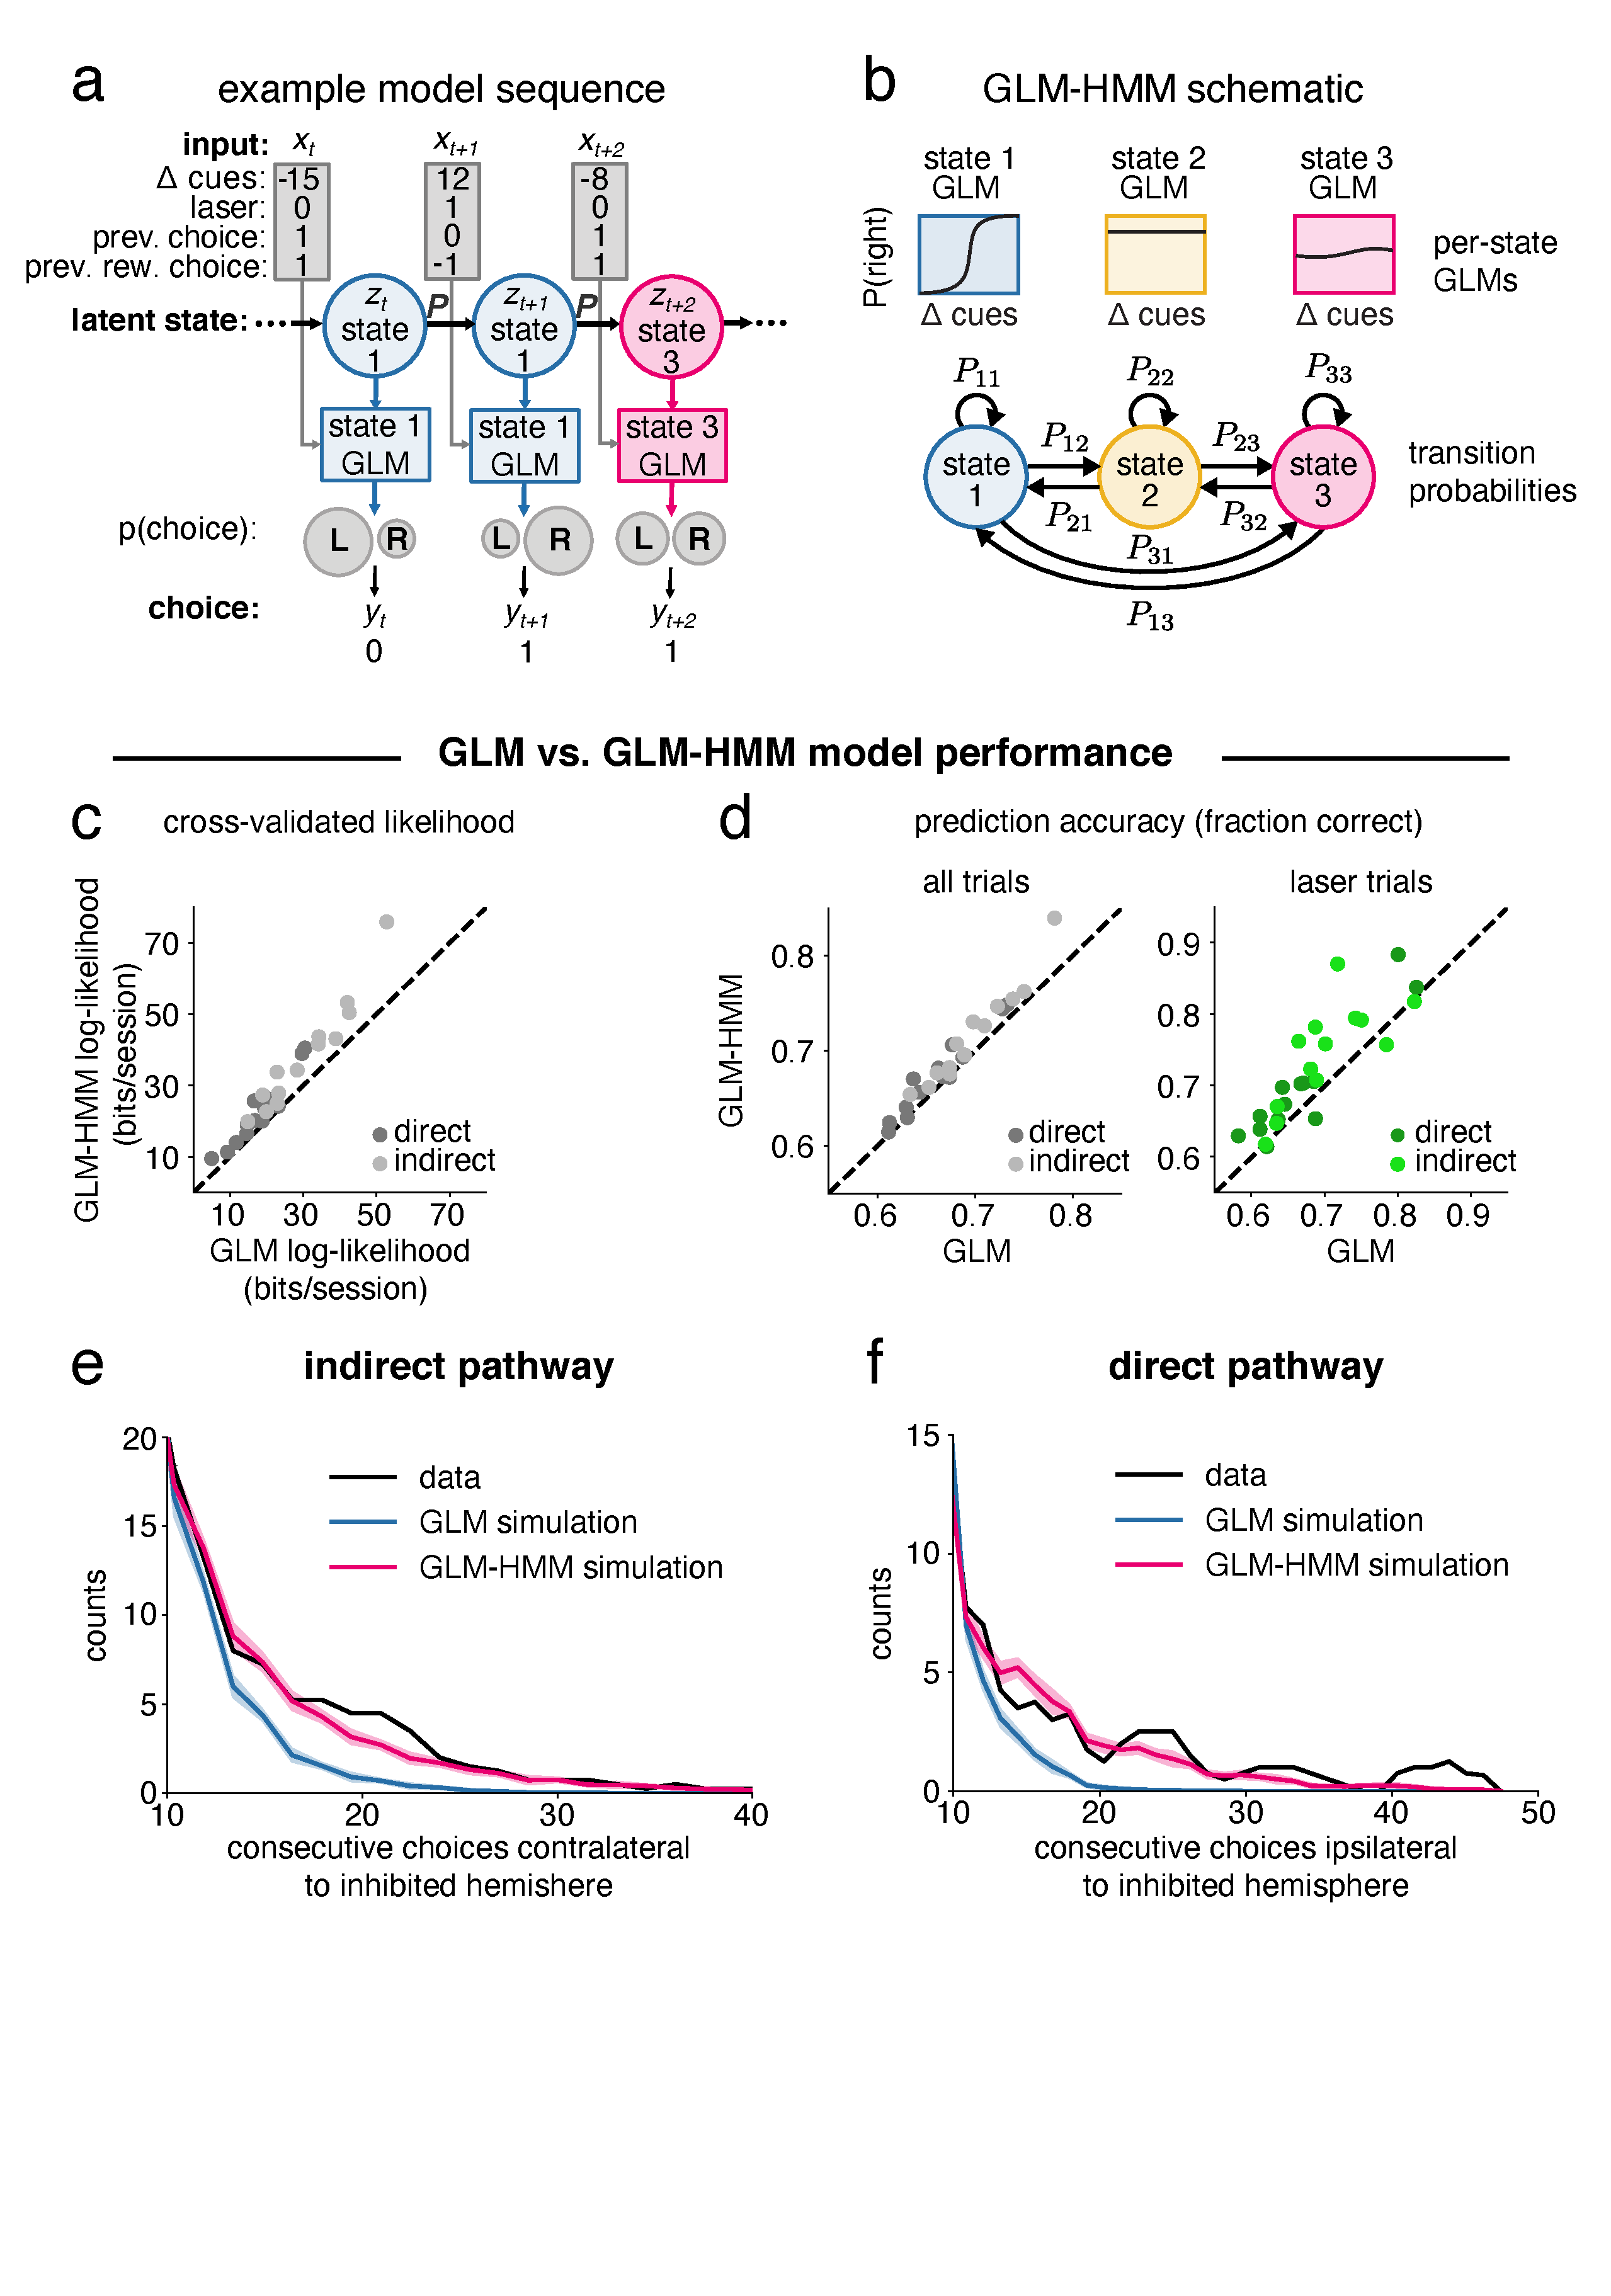
\includegraphics[width=0.90\linewidth]{ch2-glmhmm/glmhmm-figures/Fig5.pdf}
    \caption[A GLM–HMM better explains choice during the evidence accumulation task than the GLM, particularly on trials with dorsomedial striatum pathway inhibition]{\textbf{A GLM–HMM better explains choice during the evidence accumulation task than the GLM, particularly on trials with dorsomedial striatum pathway inhibition.} (a) Example sequence of 3 trials of the evidence accumulation task, showing the relationship between external covariates (inputs), latent state, and choice on each trial. On each trial, the latent state defines which GLM weights map inputs ($\Delta$ cues, laser, previous choice, and previous rewarded choice) to the probability of choosing right or left. The transition probability P governs the probability of changing states between trials. See \ref{sec:appendix1:methods} for information on how the inputs were coded. (b) Schematic of GLM-HMM. The model has 3 latent states with fixed probabilities of}
    \label{fig:glmhmm:5}
  \end{center}
  \vspace{-1.5cm}
\end{figure}
\begin{figure}[t!]
  \contcaption{transitioning between them. Each state is associated with a distinct decision-making strategy, defined by a mapping from external covariates, or inputs, such as $\Delta$ cues, to choice probability. (c) Cross-validated log-likelihood demonstrating the increased performance of the GLM-HMM over a standard Bernoulli GLM on held-out sessions. Dots represent model performance for individual mice (n=13 for each group). (d) Same as c but showing prediction accuracy as a fraction of the choices correctly predicted by each model across all trials (left) or on the subset of trials when the laser was on (right). (e) Histograms showing the number of consecutive laser trials for which the animal’s choice was in the same direction as the expected biasing effect of the laser (i.e. a choice contralateral to the laser hemisphere during DMS indirect pathway inhibition). Data (black), GLM simulation (blue), GLM-HMM simulation (pink). For the simulations, data of the same length as the real data was generated 100 times and the resulting histograms averaged. Curves denote smoothed counts using a sliding window average (window size = 3 bins). Shaded regions around the GLM and GLM-HMM curves indicate 95\% confidence intervals. (f) Same as e but for mice receiving direct pathway inhibition of the DMS, therefore laser-biased choices are defined as those ipsilateral to the hemisphere of inhibition.}% Continued caption
\end{figure}

The GLM–HMM explained the choice data in the evidence accumulation task better than the GLM across multiple measures. To compare models, we computed the test log-likelihood of each animal’s data using cross-validation with held-out sessions (three-state GLM–HMM in Fig. \ref{fig:glmhmm:5}; see Extended Data Fig. \ref{fig:ap1:ext7}a–e and \ref{sec:ap1:m10} for more information on model selection). The three-state GLM–HMM achieved an average of a 6.2 bits per session (bps) increase in log-likelihood, making an average session $\sim$76 times more likely under the GLM–HMM (Fig. \ref{fig:glmhmm:5}c). Furthermore, the GLM–HMM correctly predicted choice on held-out data more often than the GLM, especially on laser trials (Fig. \ref{fig:glmhmm:5}d; average improvement across mice of 1.6\% on all trials, 3.5\% on trials with optical inhibition and 4.1\% on trials with optical inhibition when considering only mice with at least 100 inhibition trials).

Most interestingly, the GLM–HMM was better able to capture the temporal structure in the effect of inhibition on choice. Specifically, the choice data contained long runs in which choice was consistent with the bias direction predicted by pathway-specific inhibition (‘laser’), a feature which GLM–HMM simulations recapitulated, but GLM simulations did not (Fig. \ref{fig:glmhmm:5}e,f). Thus, taken together, the GLM–HMM provided a better model of the choice data than a standard GLM, particularly on trials with pathway-specific DMS inhibition.
\subsection{GLM–HMM identifies states with varying dorsomedial striatum dependence}
\label{sec:glmhmm:2.2.8}

We examined the state-dependent weights of the GLM–HMM and found substantial differences across states in the weighting of sensory evidence, previous choice and, most intriguingly, inhibition of DMS pathways (Fig. \ref{fig:glmhmm:6}a,b). In particular, two of the three states (states 1 and 2) displayed a large weighting of sensory evidence on choice, while the ‘laser’ weight was large only in state 2. In contrast, in state 3, choice history had a larger weight than in the other states, and neither sensory evidence nor ‘laser’ had much influence on choice.

To characterize state-dependent psychometric performance, we used the fitted model to compute the posterior probability of each state given the choice data and assigned each trial to its most probable state (Fig. \ref{fig:glmhmm:6}c,d). We then examined the psychometric curves for trials assigned to each state. In state 3, performance was low (Fig. \ref{fig:glmhmm:6}g) and DMS inhibition had little effect on behavior (Fig. \ref{fig:glmhmm:6}c,d). This is consistent with the high GLM weight on choice history in this state and low weights on sensory evidence and laser (Fig. \ref{fig:glmhmm:6}a,b). This implies relatively little contribution of DMS pathways during a task-disengaged state when mice pursued a strategy of repeating previous choices rather than accumulating sensory evidence. When considered together with comparisons of the effect of pathway-specific DMS inhibition in control T-maze tasks where performance is high (Fig. \ref{fig:glmhmm:2}c) but effects of inhibition are limited (Fig. \ref{fig:glmhmm:3}f–k and Extended Data Fig. \ref{fig:ap1:ext5}b,c), this implies a dissociation between task performance and the contributions of DMS pathways to behavior.

\begin{figure}[t!]
  \begin{center}
    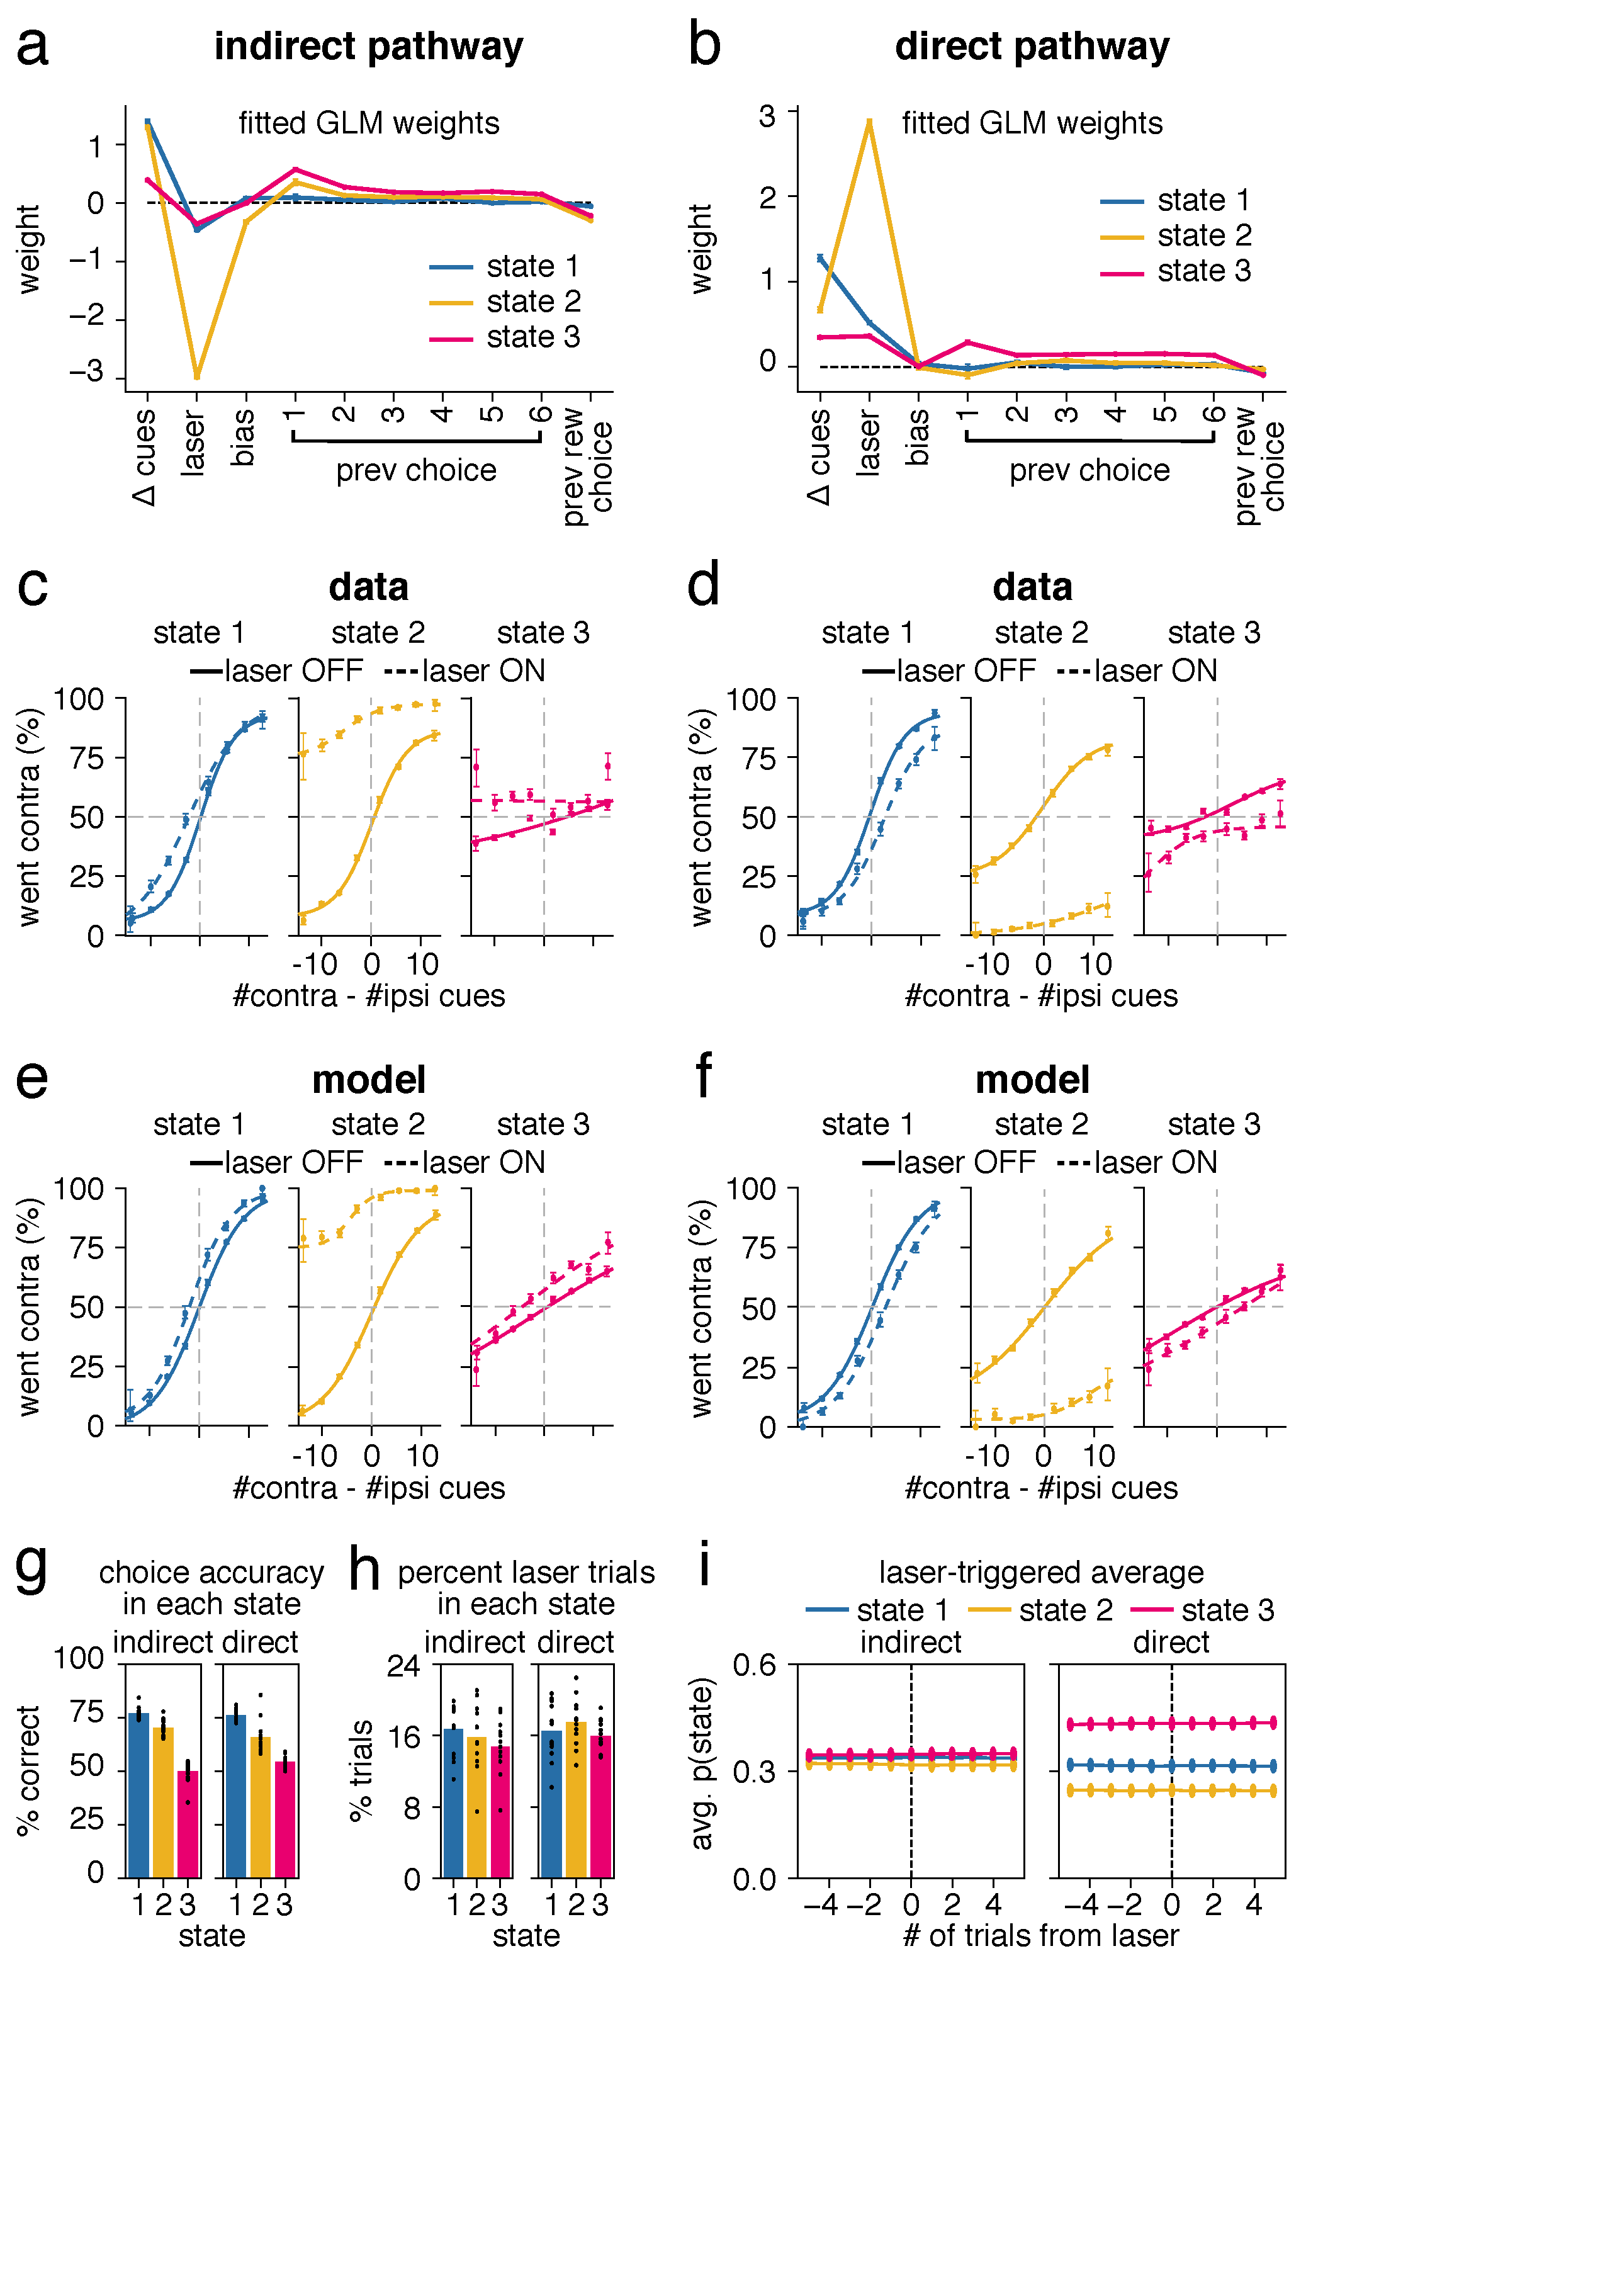
\includegraphics[width=0.80\linewidth]{ch2-glmhmm/glmhmm-figures/Fig6.pdf}
    \caption[A GLM–HMM uncovers states during the evidence accumulation task with different weighting on sensory evidence, choice history and dorsomedial striatum pathway inhibition]{\textbf{A GLM–HMM uncovers states during the evidence accumulation task with different weighting on sensory evidence, choice history and dorsomedial striatum pathway inhibition.} (a) Fitted GLM weights for 3-state model from mice in the indirect pathway DMS inhibition group. Error bars denote ($\pm$1) posterior standard deviation for each weight. The magnitude of the weight represents the relative importance of that covariate in predicting choice, whereas the sign of the weight indicates the side bias (e.g. a negative laser weight indicates that if inhibition}
    \label{fig:glmhmm:6}
  \end{center}
  \vspace{-1.5cm}
\end{figure}
\begin{figure}[t!]
  \contcaption{is in the right hemisphere, the mice will be more likely to turn left, while a positive weight on previous choice indicates that if the previous choice was to the right, in the current trial this will bias the mice to turn right again). (b) Same as a but for the direct pathway group. (c) Fraction of contralateral choices as a function of the difference in contralateral versus ipsilateral cues in each trial for mice in the indirect pathway inhibition group. To compute psychometric functions, trials were assigned to each state by taking the maximum of the model’s posterior state probabilities on each trial. Error bars denote $\pm$1 SEM  for light off (solid) and light on (dotted) trials. Solid curves denote logistic fits to the concatenated data across mice for light off (solid) and light on (dotted) trials.  (d) Same as c but for the mice receiving direct pathway inhibition of the DMS. (e) Same as c but for data simulated from the model fit to mice receiving indirect pathway inhibition of the DMS  (see \ref{sec:appendix1:methods}). (f). Same as e but for mice receiving direct pathway inhibition of the DMS. (g) Performance in each state for mice receiving DMS inhibition in the indirect pathway (left) and direct pathway (right), shown as the percentage of total trials assigned to that state in which the mice made the correct choice. Colored bars denote the average performance across all mice. Black dots show averages for individual mice (n=13 mice for both groups). (h) Percentage of laser-on trials that the model assigned to each state for mice receiving DMS inhibition in the indirect pathway (left) and direct pathway (right). Colored bars denote the average performance across all mice. Black dots show averages for individual mice (n=13 mice for both groups). (I) The posterior probability of each state for the five trials before and after a laser-on trial, averaged across all such periods (n=8570, indirect; n=7927, direct). }% Continued caption
\end{figure}

Compared to state 3, sensory evidence heavily modulated behavior in both states 1 and 2, and performance was accordingly high (Fig. \ref{fig:glmhmm:6}c,d,g). Interestingly, the effect of DMS pathway inhibition was much larger in state 2. These results were again consistent with the GLM weights: both state 1 and 2 had high weighting of sensory evidence and low weighting of choice history but greatly differed in their weighting of the ‘laser’ (Fig. \ref{fig:glmhmm:6}a,b). The discovery of state 2 implies that DMS pathways contribute most heavily to choices in a state in which mice are pursuing a strategy of evidence accumulation, consistent with cross-task comparisons of the effects of inhibition (Fig. \ref{fig:glmhmm:3}). The discovery of state 1, which differed most noticeably from state 2 in the extent that the laser affected choice, may suggest the existence of another neural mechanism for evidence accumulation with minimal DMS dependence.

We found that GLM–HMM simulations closely recapitulated these state-dependent psychometric curves (Fig. \ref{fig:glmhmm:6}e,f). This not only validated our fitting procedure but provided additional evidence that a multistate model provides a good account of the animals’ decision-making behavior during the evidence accumulation task.

While the effect of the laser differed across states, the probability of being in a particular state did not change on or after trials with optical inhibition (Fig. \ref{fig:glmhmm:6}i), implying that DMS pathway inhibition itself did not generate transitions between states. In addition, the fraction of trials with optical inhibition was equivalent across states ($\sim$15\% of all trials in each state; Fig. \ref{fig:glmhmm:6}h). This implies that the model did not identify states simply based on the presence of laser trials.

We obtained similar states when fitting the model to a combined dataset including all groups of mice (those receiving DMS indirect and direct pathway inhibition, as well as control mice receiving DMS illumination in the absence of NpHR; Extended Data Fig. \ref{fig:ap1:ext7}f). As when fitting each group separately, the combined fit revealed that both inhibition groups contained a single state with large weights on sensory evidence and the laser. In contrast, the control mice had small laser weights across all three states.

We also examined the results of fitting the four-state GLM–HMM (Extended Data Fig. \ref{fig:ap1:ext7}d,e), given it had a slightly higher cross-validated log-likelihood than the three-state model (Extended Data Fig. \ref{fig:ap1:ext7}a). In this case, the weights for states 1 and 2 were very similar to those in the three-state model; the key difference was that the choice history state (state 3 of the three-state model) was further subdivided into two states that differed in having a slight rightward versus a slight leftward bias. This suggests that while the model may uncover finer-grained structure in the data beyond three states (Extended Data Fig. \ref{fig:ap1:ext7}d,e), these states yield diminishing interpretive insight on the weighting of sensory evidence, choice history and DMS pathway inhibition across time.
\subsection{Diversity in timing and number of GLM–HMM state transitions}
\label{sec:glmhmm:2.2.9}

The fitted transition matrix revealed a high probability of remaining in the same state across trials (Fig. \ref{fig:glmhmm:7}a,b). These transition probabilities produced a diversity in the timing and number of state transitions across sessions, which we visualized by calculating the maximum posterior probability of each state on each trial (Fig. \ref{fig:glmhmm:7}c,d and \ref{sec:ap1:m10}). In some sessions, mice persisted in the same state, while in many sessions, mice visited two or even all three states (see example sessions in Fig. \ref{fig:glmhmm:7}c,d, summaries of state occupancies across sessions in Fig. \ref{fig:glmhmm:7}e–h and a summary of all individual mice in Supplementary Fig. \ref{fig:ap1:supp4}). Average single-state dwell times ranged from 39 to 86 trials (Fig. \ref{fig:glmhmm:7}g). This was shorter than the average session length of 194 trials, consistent with visits to multiple states per session.

\begin{figure}[t!]
  \begin{center}
    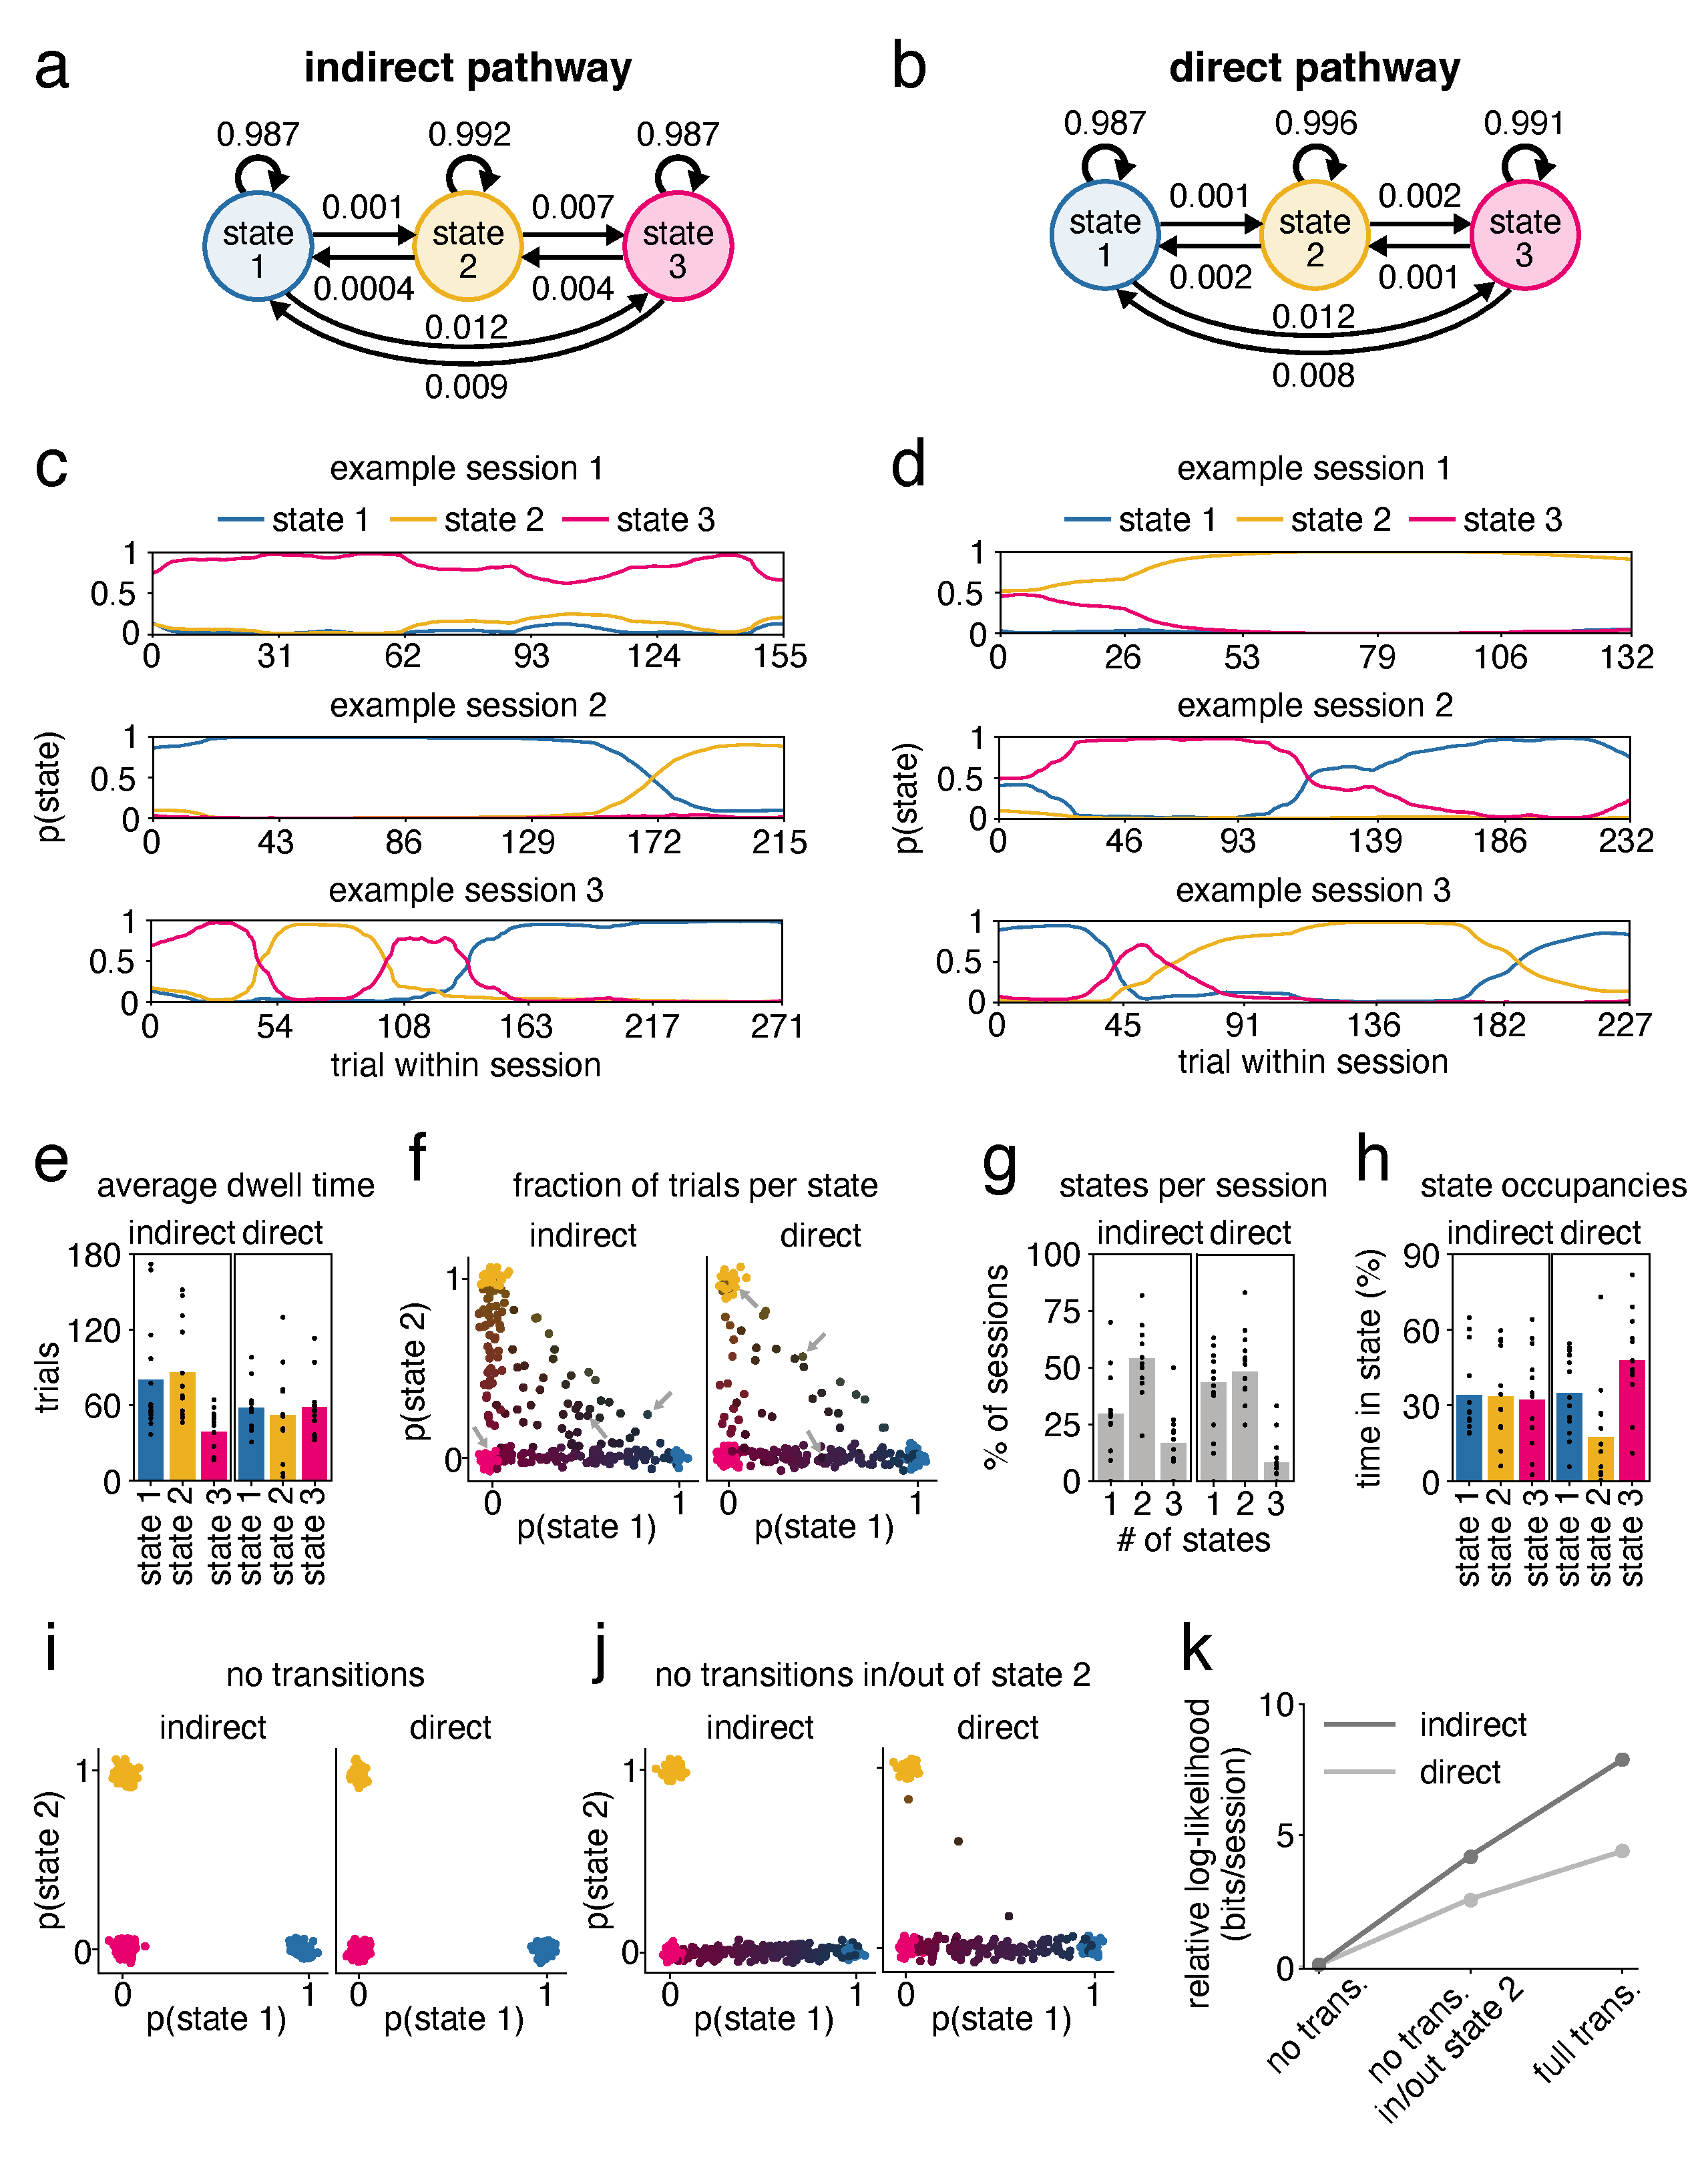
\includegraphics[width=0.90\linewidth]{ch2-glmhmm/glmhmm-figures/Fig7.pdf}
    \caption[Diversity across sessions in the timing and number of GLM–HMM state transitions]{\textbf{Diversity across sessions in the timing and number of GLM–HMM state transitions.} (a) Transition probabilities for the indirect pathway group. (b) Same as a but for the direct pathway group. (c) The posterior probability of being in each state for each trial for 3 example sessions from a mouse in the indirect pathway group. (d) Same as c but for two mice from the direct pathway group. (e) Dwell times showing the average consecutive number of trials that the mice spent in each state for mice with indirect (left; range 39-86 trials, average session length 202 trials) and direct (right; range 52-59 trials, average session length 185 trials) pathway}
    \label{fig:glmhmm:7}
  \end{center}
  \vspace{-1.5cm}
\end{figure}
\begin{figure}[t!]
  \contcaption{inhibition. Black dots show averages for individual mice (n=13 mice for both groups). (f). The fraction of trials that the mice spent in each state in each session. Each dot represents an individual session (n=271, indirect pathway; n=266, direct pathway). Color-coding reinforces the state composition of each session (e.g. blue indicates the mouse spent 100\% of the session in state 1). A small amount of Gaussian noise was added to the position of each dot for visualization purposes. Grey arrows identify the example sessions shown in c and d. (g) The fraction of sessions in which the mice entered one, two, or all three states. Gray bars denote the average fraction of sessions for all mice. Black dots show averages for individual mice (n=13 mice for both groups). (h) Time spent in each state represented as a percentage of total trials for mice inhibited in the indirect pathway (left) and direct pathway (right). Colored bars denote the average state occupancies across all mice. Black dots show averages for individual mice (n=13 mice both groups). (i) Same as f except state assignments were obtained from a model in which the transition probabilities were restricted to disallow transitions between states (i.e. all off-diagonal transition probabilities equal zero; see Methods). (j) Same as f except state assignments were obtained from a model in which transitions were disallowed between state 2 and the other states. (k) Comparison of the cross-validated log-likelihood of the data when fitting GLM-HMMs with the reduced models from i and j, relative to the log-likelihood of the full model, in bits per session. 
 }% Continued caption
\end{figure}

While individual sessions were heterogeneous in terms of their state occupancies, averaged across sessions, the posterior probability of being in each state tended to be stable across trials (Fig. \ref{fig:glmhmm:7}e and Extended Data Fig. \ref{fig:ap1:ext8}a,b). Model simulations recapitulated these state transition characteristics, including dwell times and state occupancies (Extended Data Fig. \ref{fig:ap1:ext9}), further indicating our model captures latent structure in our data.

One notable exception in the stability of posterior probabilities of each state across time was an increase in state 3 probability toward the end of a session (Extended Data Fig. \ref{fig:ap1:ext8}a), potentially reflecting a decrease in task engagement related to reward satiety. Consistent with a relationship to satiety, within-session transitions into state 3 were associated with higher amounts of previously accumulated reward and higher preceding rates of reward (Extended Data Fig. \ref{fig:ap1:ext8}c–f). In addition, while the posterior probability of each state showed minimal modulation surrounding a rewarded trial, the probability of state 3 was much more likely surrounding trials with excess travel (Extended Data Fig. \ref{fig:ap1:ext8}g–j), an indicator of non-goal-directed movement and task disengagement. Indeed, the probability of state 3 gradually increased and decreased approximately 25 trials before and following excess travel trials, consistent with the average dwell time for state 3 (Fig. \ref{fig:glmhmm:7}e).

Given the presence of sessions in which mice occupied a single state, we considered model variants that disallowed within-session state transitions. Our goal was to determine if these variant models could provide a better explanation of the data, or alternatively, if within-session state transitions are in fact an important structural feature for explaining the data. In one model variant, we disallowed transitions between states entirely (Fig. \ref{fig:glmhmm:7}k). In the other, we tested the possibility that state 2, which is unique in the strength of its laser weight, captured a session-specific feature of inhibition by disallowing transitions in and out of that state (Fig. \ref{fig:glmhmm:7}l). Using cross-validation, we found that neither alternative model explained the data as well as a model with unrestricted transitions (Fig. \ref{fig:glmhmm:7}m), indicating that within-session transitions between states was an important feature of the model.


\subsection{Motor performance across GLM–HMM states}
\label{sec:glmhmm:2.2.10}

Given the close relationship between excess travel and the posterior probability of state 3, we considered the possibility that other measures of motor behavior varied across states. We found that on trials without DMS pathway inhibition (Extended Data Fig. \ref{fig:ap1:ext10}a–g,o–u), mice exhibited no obvious differences across states in velocity, x-position or view angle (Extended Data Fig. \ref{fig:ap1:ext10}a–d,o–r). However, during state 3 relative to state 1 and 2, we observed an increased tendency in measures of non-goal-directed movements (Extended Data Fig. \ref{fig:ap1:ext10}e–g,s–u). This is consistent with the higher probability of state 3 around trials with excess travel (Extended Data Fig. \ref{fig:ap1:ext8}h,j), and the interpretation of state 3 as a task-disengaged state.

We also considered the possibility that DMS pathway inhibition had state-dependent effects on motor output (Extended Data Fig. \ref{fig:ap1:ext10}h–n,v–bb). We observed limited effects of inhibition on velocity, per-trial standard deviation in view angle and distance traveled across all three states. However, similar to our cross-task comparisons (Extended Data Fig. \ref{fig:ap1:ext6}j,k), DMS pathway inhibition produced a small but opposing bias in average x-position (Extended Data Fig. \ref{fig:ap1:ext10}j,x) and view angle (Extended Data Fig. \ref{fig:ap1:ext10}k,y), which was greatest in the state with the largest laser weight (state 2; Fig. \ref{fig:glmhmm:6}). This is consistent with our conclusions that the effects of DMS inhibition on behavior are state dependent, and that x-position and view angle are closely linked indicators of choice in the context of VR-based T-maze tasks (Extended Data Fig. \ref{fig:ap1:ext3}g–j).
\section{Discussion}
\label{sec:glmhmm:discussion}



\chapter{Identification of the dynamic structure underlying naturalistic behaviors\label{ch:slds}}

\section{Introduction}
\label{sec:slds:introduction}

In order to analyze and understand an animal's behavior, or the sequential set of actions that it elicits through its bodily movements over a period of time, we must first have a consistent and reliable way to track those body poses in both time and space. Meeting this objective has been one of the central goals of scientists working at the intersection of neuroscience, ethology, machine learning, and computer vision over the past decade. The result has been an explosion of work that takes in recordings (typically in the form of video data) of behaving animals and outputs a continuous-time representation of the animals' actions in space \cite{toshev_deeppose_2014, tompson_joint_2014, newell_stacked_2016, cao_realtime_2017, mathis_deeplabcut_2018, pereira_fast_2019, batty_behavenet_2019, graving_deepposekit_2019, bohnslav_deepethogram_2021, marshall_continuous_2021, dunn_geometric_2021, lin_characterizing_2022, sun_self-supervised_2022, pereira_sleap_2022, chen_alphatracker_2023}. These representations often take the form of time-series of ``keypoints," or specific points of interest identified on the body, such as the paws, nose, and tail. 

However, obtaining these time-series representations is just the first step in the process of thoroughly describing an animal's behavior. The next step is to take the results of keypoint tracking and use statistical machine learning models to cluster the data into discrete modules, which can then serve as fundamental units for identifying and interpreting more complex and long-lasting sequences of behavior -- much like we understand language by organizing individual letters into longer structures of syllables, words, sentences, and so on. While there are about as many approaches to behavioral clustering as there are to keypoint estimation, one method that rose to early popularity is a latent variable model known as the autoregressive hidden Markov model, or AR-HMM \cite{bryan_autoregressive_2015}. 

In basic design, an AR-HMM is much like the GLM-HMM discussed in Chapter \ref{ch:glmhmm}. However, in this case, the observational data is some representation of the animal's pose positions at each time point, instead of binary choices; the inputs are the postural data from the previous time point (thus the ``autoregressive" nature of the model), instead of task variables; and because the observations are Gaussian rather than Bernoull-distributed, the mapping between the inputs and choices in each state is linear rather than sigmoidal. When applied to behavioral quantification problems, past applications of AR-HMMs have used depth-imagining video data as the model observations, rather than extracted keypoints \cite{wiltschko_mapping_2015, markowitz_striatum_2018, wiltschko_revealing_2020}. This approach is effective in that the pixels from depth cameras are relatively smoothly-varying in time, leading to learned state representations of long duration (relative to the sampling rate) that readily correspond to identifiable, interpretable behaviors. However, a drawback of this method is that the low-resolution of the depth video data limits the precision and detail of discoverable behaviors. To fully characterize the repertoire of animal behavior, it is thus necessary to employ models that directly leverage keypoint data, which captures postural information at higher resolution. 

In this chapter, we address this need by first fitting an AR-HMM to keypoint data -- extracted using SLEAP \cite{pereira_sleap_2022} -- from videos of mice freely exploring a linear track. We identify some crucial shortcomings in the outcome this approach, namely that the state sequences flicker rapidly in a manner much faster than the animal's behavior. This result has also been observed in other recent work \cite{wu_deep_2020, luxem_identifying_2022}. Hypothesizing that this problem is due to noise in the estimates of the keypoint positions (which vary less smoothly across time than the pixels from depth-imaging cameras), we instead employed a switching Linear Dynamical System (sLDS) model, which is akin to an AR-HMM except that there is an additional layer of continuous latent states between the observations and the discrete states \cite{ackerson_state_1970, chang_state_1978, fox_nonparametric_2008, murphy_machine_2012, linderman_bayesian_2017}. Whereas the observations are the keypoint coordinates themselves, the continuous latents represent denoised keypoints that allow for discrete state inference that is less affected by jitter in the observations. This results in state sequences that correspond much more closely to expected durations of animal behavior \cite{wiltschko_mapping_2015} and readily map on to identifiable actions such as sitting, walking, and rearing. 

Despite the advantages of using an sLDS over an AR-HMM in terms of model performance and interpretability, one major drawback is the computational time required to fit sLDS models; this is largely due to the need to jointly infer the discrete and continuous state trajectories and the move from an exact to an approximate loss function. This time cost is magnified by the fact that inference in both AR-HMMs and sLDS models relies on iterative fitting procedures such as the Expectation Maximization (EM) algorithm \cite{baum_maximization_1970, dempster_maximum_1977, shumway_approach_1982, bishop_pattern_2006, escola_hidden_2011}. EM is not guaranteed to find the optimal solution for a given model fit; Therefore, a typical approach is to fit the model several times and take the best solution as evidence of having found the global optimum. However, the results of each fit are highly dependent on the values at which the system parameters are initialized, and poor initializations can add to the time-inefficiencies of this method. Conversely, smart initializations, in which the starting guess of the system parameters is close to the true ones, can greatly speed up fitting. Here, we attempt to devise a method for obtaining smart initializations for sLDS models by extending existing ideas for the general linear-Gaussian LDS case from spectral learning \cite{martens_learning_2010, anandkumar_tensor_2014, belanger_linear_2015, hazan_learning_2017, hazan_spectral_2018} and subspace identification \cite{ho_editorial_1966, van_overschee_n4sid_1994, viberg_subspace-based_1995, van_overschee_subspace_1996, qin_overview_2006} to be applicable to the discrete state switching regime. 


% However, when applied to keypoint data, MoSeq failed to identify syllables at this
% characteristic ~400ms timescale, instead producing a set of brief syllables (<100 ms)
% together with a small number of aberrantly long syllables that merged multiple
% behaviors; furthermore, the transitions between these syllables aligned poorly to
% changepoints derived from the keypoint data (Fig. 2a-b). These observations are
% consistent with prior work demonstrating that feeding keypoints to MoSeq generates
% behavioral representations that are less informative than those generated by alternative
% clustering methods13,22. 
\section{Results}
\label{sec:slds:results}



\section{Discussion}
\label{sec:slds:discussion}

Behavioral segmentation and quantification is a topic of keen interest to the neuroscience community for its potential to precisely and reliably map observable actions to underlying representations of neural activity. The best computational methods for achieving this goal is an open question and active area of exploration amongst researchers, and the answer may depend on behavioral context, data characteristics, and questions of interest. Latent variable models are one class of methods that have become particularly popular because their underlying statistical structure reflects the exact brain-behavior relationship that neuroscientists hope to capture: a time series of observable variables (behavior) governed by an underlying dynamic process that may evolve in a continuous and/or discrete manner over time and is hidden from direct observation (brain activity). However, the full utility of these models and their generalizability across contexts, data, and questions remains to be seen.  

Here we have presented two latent variable models for quantifying mammalian behavior and compared their performance in identifying basic behavior states as mice explore a linear track. The first, an AR-HMM, is the more familiar approach in the literature \cite{wiltschko_mapping_2015, markowitz_striatum_2018, wiltschko_revealing_2020, costacurta_distinguishing_2022}. The second, an SLDS, can be seen as an extended version of an AR-HMM with an additional state layer that represents a denoised projection of the low-level observations. We compared the two models across both quantifiable and qualitative metrics to assess measures such as their accuracy in identifying ground-truth behaviors as well as their ability to capture states that reflect interpretable, distinct types of actions. 

Our findings indicate that the SLDS performs better than the AR-HMM across most measures. Average discrete state durations are longer and self-transition probabilities higher, especially for stationary behaviors. This is likely due to the denoising component of the SLDS, as it enables capture of long periods when the mouse is not moving without being artificially disrupted by noise in the keypoint positions. States are also more distinguishable from one another in terms of the animals' average pose and sideways and upwards velocities in each state. Mapping these states back onto the video recordings, the SLDS states can be more readily associated with different behaviors (i.e. stationarity and combinations of movements at differing speeds) than the AR-HMM inferred states, which don't clearly cluster into any distinct behaviors. 

Direct model comparisons further support the superiority of the SLDS model. The SLDS performs better at predicting the true states (compared to ground truth labels) on test data and reports lower errors than the AR-HMM. It also does a much better job at classifying stationary behavior, though it does somewhat worse at distinguishing between two different movement behaviors (rearing and walking). 

While the results show high potential for the use of SLDS models in behavioral quantification, they also reveal several areas of improvement. The average state durations are still much shorter than what is typically associated with discrete behaviors \cite{wiltschko_mapping_2015}. This may speak to the need to refine the magnitude of the latent noise term in order to further reduce jitter in the observations or to impose a dynamic noise term that varies over time in accordance with the amount of observed noise in the keypoints. One recent attempt to implement the latter has garnered positive results, with average state durations approaching 400ms \cite{weinreb_keypoint-moseq_2023}. 

Another limitation in our SLDS model is that the behaviors associated with the inferred non-stationary states are neither sufficiently well distinguished nor score well in their precision and recall of ground truth behaviors. This problem is likely solveable by adding a velocity term as an input to the model (possibly with separate velocity terms for different axes) to help distinguish the pose trajectories associated with different behaviors. Early evidence suggests that including at least a centroid velocity term, along with the animal's heading direction in order to capture overall position in allocentric coordinates, helps to distinguish between different types of locomotion such as walking, rearing, and turning \cite{weinreb_keypoint-moseq_2023}. 

There are of course additional considerations to optimize SLDS performance, including adding discrete states to uncover more behaviors and using cross-validation or singular value decompositions of the data to determine the appropriate dimensionality of the continuous states. It is likely that the model would produce equivalent or even superior results with a continuous latent space that is of reduced dimension relative to the observation space, preserving only the most relevant information to infer the discrete state behavioral dynamics. Reducing the number of continuous latent dimensions can also vastly speed up inference, which is a substantial problem in fitting SLDS models. 

Another factor that influences fitting efficiency is the parameter scheme used to initialize model inference. One approach is to generate initial parameters using a combination of factor analysis and/or AR-HMMs to obtain estimates of the continuous and discrete state dynamics \cite{linderman_recurrent_2016, linderman_hierarchical_2019, weinreb_keypoint-moseq_2023}. However, fitting AR-HMMs to keypoint data does not produce state sequences reflective of the data, as has been shown here and elsewhere \cite{wu_deep_2020, luxem_identifying_2022, weinreb_keypoint-moseq_2023}. Therefore, alternative approaches to SLDS initialization, such as the fastSLDS method we propose here, will be important to explore more thoroughly as wide spread adoption of SLDS models for behavioral quantification becomes likely.  

Altogether, this work provides an important examination of two latent variable models for behavioral quantification and raises critical questions about the right computational tools for extracting relevant information from behavioral data. We also suggest essential considerations about the efficiency of fitting such models and propose a novel solution to reduce inference time. To this end, we expect our work to provide a useful foundation for future studies to expand upon as the field pinpoints the optimal techniques for modeling behavioral data and linking its dynamic structures to underlying patterns of neural activity. 


\chapter{Spectral learning of Bernoulli linear dynamical systems models\label{ch:bestlds}}

\section{Introduction}
\label{sec:bestlds:intro}

Latent linear dynamical system (LDS) models are an important and widely-used tool for characterizing the structure of many different types of time series data, including natural language sequences \cite{belanger_linear_2015}, task-guided exploration \cite{wagenmaker_experimental_2021}, and neural population activity \cite{gao_high-dimensional_2015,nonnenmacher_extracting_2017, zoltowski_general_2020}. To fit these models, the typical approach is to use an inference method such as the expectation maximization (EM) algorithm in order to find a local maximum of the likelihood function \cite{escola_hidden_2011}. However, such inference methods are often time-consuming, computationally expensive, and provide no guarantee of finding the global optimum. To address these issues, an active area of research has emerged using spectral methods to identify the parameters of linear time invariant (LTI) systems from input-output data \cite{martens_learning_2010, anandkumar_tensor_2014, belanger_linear_2015, hazan_learning_2017,hazan_spectral_2018}. Such methods rely on an approach from control theory known as subspace identification (SSID), which uses moment-based estimation to fit the model parameters without the need for an iterative procedure \cite{ho_editorial_1966,van_overschee_n4sid_1994,viberg_subspace-based_1995,van_overschee_subspace_1996,qin_overview_2006}. The resulting parameter estimates are consistent and avoid the problem of local optima that are common with inference methods such as EM, although they typically suffer from lower accuracy. Therefore, a common strategy is to combine both approaches, using the SSID estimates as initializations for EM in order to speed convergence and increase the likelihood of finding the global optimum. 

Most recent developments in spectral estimation methods for LDS models have focused on undriven (no inputs) linear-Gaussian observation processes. However, there has been work extending SSID for LDS models to handle Poisson observations, which is a useful framework for modeling neural spike-train data at certain timescales (e.g. $>10$ms), as well as developing the general case for input-driven models \cite{buesing_spectral_2012}. Yet there is a need for additional research explicitly expanding spectral methods to other distribution classes. For example, binary time series data are common in many fields, including reinforcement learning and decision-making. While there has been some work exploring second-order models for binary variables \cite{bethge_near-maximum_2008, macke_generating_2009, schein_poisson-gamma_2016}, there have been few attempts to develop a spectral learning method for LDS models with Bernoulli observations. Such a method would be extremely useful for identifying the dynamics of any binary time series data, including sequences of choice behavior and neural spike-trains with small bin sizes. In addition, recovery accuracy of the input-related parameters has not been well-characterized for non-Gaussian emissions models.

Here, we achieve two main innovations. First, we extend the SSID method to the probit-Bernoulli LDS case, deriving a new estimator: bestLDS (BErnoulli SpecTral Linear Dynamical System). From a technical perspective, this involves overcoming difficulties due to redundancies in the moments that are not present in the Poisson or general cases. We show this method yields consistent estimates of the model parameters when fit to input-output data from a wide range of simulated datasets. Furthermore, we demonstrate that using the outputs from bestLDS as initializations for EM significantly accelerates convergence. Second, we present new analyses, looking at parameter recovery error for the input-related LDS parameters as well as incorporating model-comparison metrics for the model as a whole. To our knowledge, neither of these analyses has been conducted on LDS models with non-Gaussian emissions. Lastly, we demonstrate the benefits of this method when applied to the behavior of mice performing a perceptual decision-making task.

\section{Background and Related Work}
\label{sec:bestlds:background}

\subsection{Applications of state-space models in neuroscience}
\label{sec:bestlds:background:applications}

LDS and related state-space models have a long history in neuroscience. Bernoulli- and Poisson-LDS models have been particularly popular for inferring latent processes underlying neural spike trains \cite{gao_high-dimensional_2015, nonnenmacher_extracting_2017, zoltowski_general_2020, valente_probing_2022}. LDS models are also useful for linking neural dynamics to animal behavior \cite{linderman_hierarchical_2019}, while discrete state-space models like hidden Markov models (HMMs) have become increasingly common tools for characterizing behavior directly \cite{wiltschko_mapping_2015, calhoun_unsupervised_2019, wiltschko_revealing_2020}. More recently, there has been growing interest in using state-space models to describe behavior: (1) using  continuous rather than discrete variables \cite{johnson_composing_2016, costacurta_distinguishing_2022}; (2) specifically in two-alternative forced-choice (2AFC) decision-making contexts \cite{roy_extracting_2021};  and (3) while understanding the affects of inputs such as sensory stimuli \cite{calhoun_unsupervised_2019, bolkan_opponent_2022, ashwood_mice_2022}. Bernoulli-LDS models lie at the intersection of all three objectives, and thus their utility (along with methods that make their inference more efficient) will likely be central to neuroscience research in the future.
\subsection{Extensions to LDS models}
\label{sec:bestlds:background:extensions}

In addition to standard approaches, there has also been substantial work extending LDS models to more flexible dynamical systems in order to better capture important features in neuroscience data. For example, Gaussian-process factor analysis (GPFA) was developed to provide insight into neural signals by extracting smooth, low-dimensional trajectories from recorded activity \cite{yu_gaussian-process_2009}. Building on GPFA, Orthogonal stochastic linear mixing models (OSLMMs) relax the assumption that correlations across neurons are time-invariant and provide innovations in the regression framework that makes inference more tractable for large datasets \cite{meng_bayesian_2022}. Other approaches employ LDS models as constituents of multi-component frameworks in order to capture more complex temporal activity patterns in neural data. One class of examples includes latent factor analysis via dynamical systems (LFADS) and its extensions, which use recurrent neural networks (RNNs) to recover neural population dynamics \cite{pandarinath_inferring_2018, prince_parallel_2021, zhu_deep_2022}. Another approach employs variants of switching linear dynamical systems (sLDS), which learn flexible, non-linear models of neural and behavioral data by treating activity as sequences of repeated dynamical modes \cite{linderman_hierarchical_2019, nassar_tree-structured_2019, zoltowski_general_2020, mudrik_decomposed_2022, wang_bayesian_2022, weinreb_keypoint-moseq_2023}. These advances make clear that LDS models serve a valuable and fundamental purpose in neuroscience and will continue to act as an essential building block for future work. 
\subsection{Inference methods}
\label{sec:bestlds:background:inference}

Fitting an LDS (as well as any of the extensions mentioned above) requires inferring the parameters governing the latent dynamics and emissions of the system. The most common approaches to inference are the Expectation Maximization (EM) algorithm \cite{baum_maximization_1970, dempster_maximum_1977, shumway_approach_1982, escola_hidden_2011} and Markov Chain Monte Carlo (MCMC)  methods \cite{metropolis_equation_1953, hastings_monte_1970, geman_stochastic_1984, gelfand_sampling-based_1990}. MCMC is a simulation method that produces samples that are approximately distributed according to the posterior; these samples are then used to evaluate integrals once convergence is reached. One of the benefits of MCMC is that it tends to work even for complicated distributions. However, it is often difficult to assess accuracy and evaluate convergence. MCMC is also slow and tends to require a large number of samples. EM, on the other hand, is an iterative optimization technique that returns a local maximum of the likelihood. EM is advantageous for a number of reasons, including that the "M-step" equations (in which parameter values are updated) often exist in closed form, the value of the likelihood is guaranteed to increase after each iteration of the algorithm, and in many cases EM requires fewer samples than MCMC. Several flexible variants of EM also exist. For example, when the conditional expectation of the log-likelihood is intractable, it is possible instead to use numerical approaches or to compute an analytical approximation using a technique such as Laplace's method \cite{steele_modified_1996} or variational inference \cite{blei_variational_2017}. In this case, optimization occurs over an "Evidence Lower Bound" (ELBO) of the likelihood of the observed data. Despite these benefits, one major drawback of EM is that it is only guaranteed to find a local maximum. Thus, it often takes multiple initializations (or else a smart choice of initial parameters) to effectively find the global maximum. For this reason, methods such as bestLDS that identify good initializations for EM stand to greatly improve its computational efficiency. This is in contrast to MCMC, wherein it is typical to discard the first several samples (due to being poor representations of the posterior distribution) and therefore the initialization scheme is less important.
\subsection{Initialization approaches for EM}
\label{sec:bestlds:background:initialization}

Given the impact that the choice of initialization has on EM performance, it's no surprise that there is an extensive body of work on "smart" EM initialization methods for a variety of state-space models, including both LDS models \cite{buesing_spectral_2012, hazan_learning_2017, hazan_spectral_2018} and HMMs \cite{siddiqi_reduced-rank_2010, hsu_spectral_2012, anandkumar_tensor_2014, liu_efficient_2017, mattila_identification_2017}. Often, these techniques rely on a combination of moment-based estimators \cite{martens_learning_2010, buesing_spectral_2012, hsu_spectral_2012, anandkumar_tensor_2014, mattila_identification_2017} and subspace identification methods \cite{ho_editorial_1966, van_overschee_n4sid_1994, viberg_subspace-based_1995, van_overschee_subspace_1996, andersson_subspace_2009, qin_overview_2006}. Despite this work, a significant gap has persisted in that these methods (1) often don't account for input-driven data and (2) do not work for binomial distributions. BestLDS addresses both of these shortcomings. Although there have been several developments for augmented approaches to EM in logistic models using Polya-Gamma latent variables \cite{polson_bayesian_2013, schein_poisson-gamma_2016}, these methods address other inference challenges in binomial-distributed data rather than improvements in the initialization scheme. However, it will be an interesting case for future study whether bestLDS can be combined with these methods to further improve inference for logistic models.
\section{Theory}
\label{sec:bestlds:theory}

\subsection{Model description}
\label{sec:bestlds:theory:model}

Let $y_t$ denote the $q$-dimensional observation at time $t$. Concretely, we assume that $y_t$ is emitted as Bernoulli noise from a latent dynamical system with $p$-dimensional linear-Gaussian dynamics, potentially driven at each time-step by an $m$-dimensional input $u_t$. That is:
\begin{align}
\begin{split}
    x_0 &\sim \mathcal{N}(\mu_0, Q_0) \\
    x_t \mid x_{t-1} &\sim \mathcal{N}(Ax_{t-1} + Bu_t, Q) \\
    z_t &= Cx_t + Du_t \\
    y_t \mid z_t &\sim \textrm{Bernoulli}(f(z_t))
\label{generative_model}
\end{split}
\end{align}
\noindent where $\mu_0, Q_0$ parameterize the initial distribution for the latent variable, $A$ and $B$ refer to the autoregressive and input-driven components of the mean of the latent dynamics, and $Q$ is the covariance of the latent Gaussian noise. The quantity $z_t$ is a latent convenience variable describing the state of the LDS in the $q$-dimensional output space as a linear transformation of the latent state by the output matrix $C$ and the input-output interactions matrix $D$. Finally, the outputs are sampled from a Bernoulli distribution with mean $f(z_t)$ for an arbitrary function $f$ (generally taken to be either the logistic or probit function). (Figure~\ref{fig:bestlds:1} shows a model schematic.)
\begin{figure}[t!]
\centering
    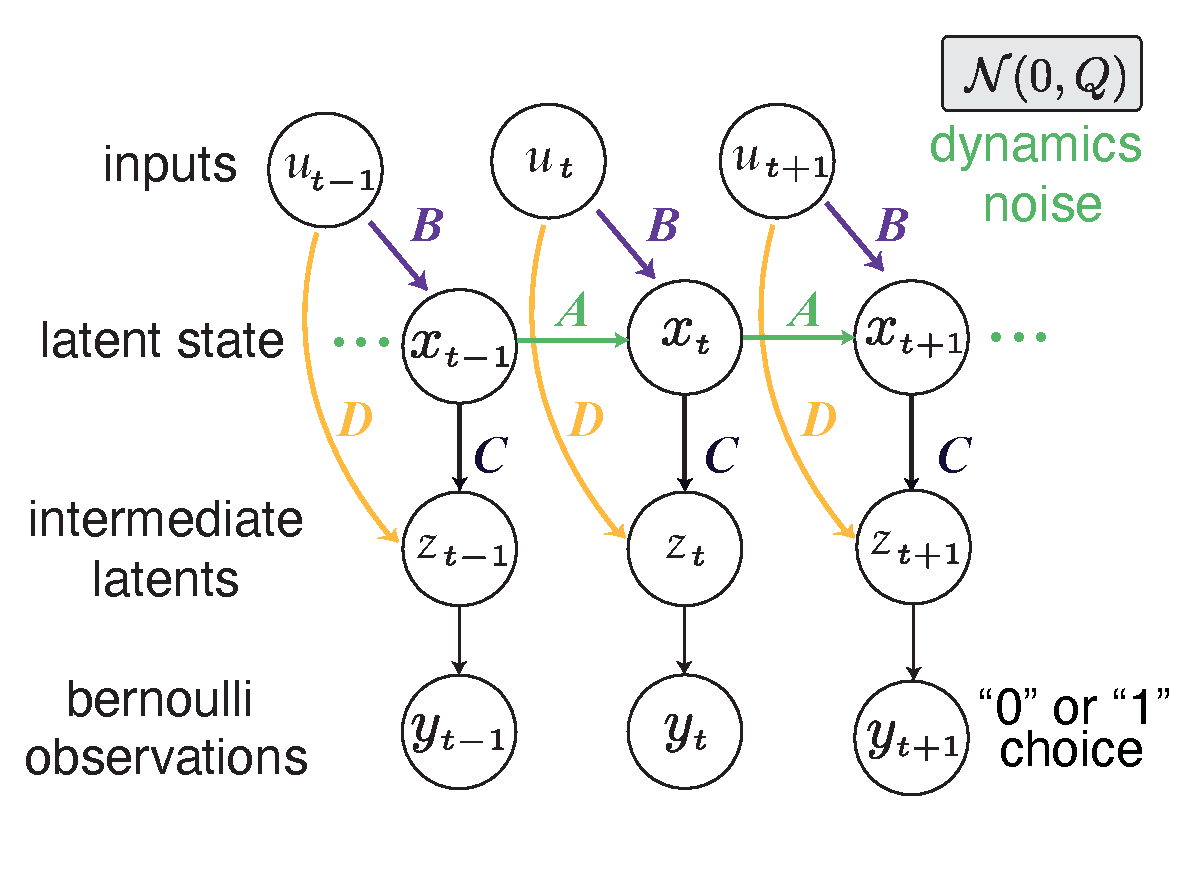
\includegraphics[width=0.65\linewidth]{ch4-bestlds/bestlds-figures/fig1.pdf}
    \caption[Generative model schematic]{\textbf{Generative model schematic.}}
    \label{fig:bestlds:1}
  %\vspace{-1.0cm}
\end{figure}
\subsection{Subspace identification}
\label{sec:bestlds:theory:subspace}

In general, subspace identification algorithms operate by first extracting an estimate of the latent state and then using linear regression to identify the system parameters. Concretely, given the latent state sequence $(x_1, ..., x_N)$ and the inputs $(u_1, ..., u_N)$ one may identify $A$ and $B$ by least-squares regression, using $(x_1, ..., x_{N-1})$ and $(u_1, ..., u_{N-1})$ to predict $(x_2, ..., x_N)$. Furthermore, given $(x_1, ..., x_N), (u_1, ..., u_N),$ and the emissions $(z_1, ..., z_N)$, one can again use least-squares to compute $C$ and $D$.

In order to achieve this, subspace identification algorithms typically operate on quantities called block-Hankel matrices, consisting of time-lagged subsequences of input or ouput data. For example, in the linear-Gaussian case, the input and output\footnote{Here we overload $z$ from Eq.~\ref{generative_model} to refer to the output, as $z$ can be seen as the emission of a linear-Gaussian LDS.} block-Hankel matrices are defined as:
\begin{align*}
    Z_{0|2k-1} &\equiv 
        \begin{pmatrix}
            z_0 & z_1 & ... & z_{N' - 1} \\
            z_1 & z_2 & ... & z_{N'} \\
             & & \vdots & \\
            z_{2k - 1} & z_{2k} & ... & z_{2k + N' - 2}
        \end{pmatrix} 
        \equiv \begin{pmatrix}
            Z_{0| k-1} \\
            Z_{k | 2k - 1}
        \end{pmatrix} 
        \equiv \begin{pmatrix}
            Z_p \\
            Z_f
        \end{pmatrix} \\\\
\end{align*}
\begin{align*}
    U_{0|2k-1} &\equiv 
         \begin{pmatrix}
             u_0 & u_1 & ... & u_{N' - 1} \\
             u_1 & u_2 & ... & u_{N'} \\
              & & \vdots & \\
             u_{2k - 1} & u_{2k} & ... & u_{2k + N' - 2}
         \end{pmatrix} 
         \equiv \begin{pmatrix}
             U_{0| k-1} \\
             U_{k | 2k - 1}
             \end{pmatrix} 
        \equiv \begin{pmatrix}
             U_p \\
             U_f
         \end{pmatrix}
\end{align*}

Note that each $z$ and $u$ above is typically a (column) vector, so these are  \textit{block} matrices. The top half of $Z_{0|2k-1}$ and $U_{0|2k-1}$ (i.e., containing rows $0$ through $k-1$) represent the ``past'' relative to the $k$th row; for simplicity we denote these $Z_p$ and $U_p$, respectively.  The bottom half of each matrix, by contrast, represents the ``future'', which we denote by $Z_f$ and $U_f$, respectively. Note that if $N$ is the total number of data points, $N' = N - 2k + 2$ is the number of columns of the matrix. Finally, the time lag parameter $k$ may be called the Hankel size and is defined by the user with only the requirement that $k \geq p$~\cite{katayama_subspace_2005}. An in-depth description of this is beyond the scope of this article, but it can be shown that only the top $p$ singular values of the Hankel matrix are greater than zero. Correspondingly, a typical heuristic is to build the Hankel matrix with large initial $k$ and then look at its singular value spectrum to pick a smaller $k$ more reflective of the underlying dynamics. 

In order to see how the block-Hankel matrix relates to the system parameters, we repeatedly expand the linear-Gaussian components of  Eq.~\ref{generative_model} to yield:
$$
Z_p = \Gamma_k \begin{pmatrix}
    x_0 & ... & x_{N' - 1}
\end{pmatrix} + \Psi_k U_p
$$
$$
\Gamma_k = \begin{pmatrix}
        C \\
        CA \\
        CA^2 \\
        \vdots \\
        CA^{k - 1}
    \end{pmatrix} 
    \qquad
    \Psi_k = \begin{pmatrix}
        D & 0 & ... & 0 \\
        CB & D &  ... & 0 \\
        \vdots & & & \vdots \\
        CA^{k - 2}B & ... & CB & D
    \end{pmatrix}
$$

where $\Gamma_k$ and $\Psi_k$ are referred to as the extended observability and controllability matrices, respectively. An analogous relationship holds for $Z_f$ and $U_f$. 

Different subspace identification algorithms are characterized by their approach to decomposing the Hankel matrix in order to extract the system parameters. In our case, we will use the N4SID algorithm \cite{van_overschee_n4sid_1994}. Briefly, this involves computing the RQ decomposition of the data matrix:
\begin{align}
    \begin{pmatrix}
        U_p \\
        U_f \\
        Z_p \\
        Z_f
    \end{pmatrix} = RQ^T
    \label{LQ_decomp}
\end{align}

It can be shown that processing various sub-blocks of the matrix $R$ permits extraction of the latent state sequence or the observability/controllability matrices, either of which can then be used to recover each of the system parameters \cite{ho_editorial_1966, van_overschee_n4sid_1994, van_overschee_subspace_1996, qin_overview_2006}. 
\subsection{Moment conversion}
\label{sec:bestlds:theory:moment}

In the Bernoulli case we do not have access to $\{z_t\}$, the ``intermediate emissions'' that arise from the linearly transformed latents,   and therefore cannot directly construct $Z_p$ or $Z_f$ as described above. However, we \textit{are} able to infer their moments from the moments of $Y_p$ and $Y_f$ (defined analogously), which has been shown in the general case to be a sufficient proxy for use in SSID methods \cite{buesing_spectral_2012}. 


In particular, let $z_p$ denote $(z_0, ..., z_{k - 1})^T$ and $z_f$ denote $(z_k, ..., z_{2k - 1})^T$, and define $u_p, u_f$ analogously. 
Then the covariance of these concatenated matrix-valued random variables has a form that allows us to recover $R$ in Eq.~\ref{LQ_decomp} via Cholesky decomposition: 
%may be approximated by computing the empirical covariance
\begin{equation}
    \label{cholesky}
    \Sigma = \mathrm{cov}\Bigg[\begin{pmatrix}
        u_p\\
        u_f\\
        z_p\\
        z_f
    \end{pmatrix}\Bigg]   
    \; = \;  RR^T.
\end{equation}
%where we achieve the last line by taking the Cholesky decomposition of $\Sigma$. 
Here, we are exploiting the fact that while the observations are not Gaussian, the intermediate emissions $z$, and their time-lagged representations $z_p$ and $z_f$, are Gaussian. This requires us to place an assumption of normality on the inputs, but we will show empirically that parameter recovery is good even when this assumption is violated (see Section~\ref{sec:bestlds:results:4.2}). For now, we begin by describing how to convert the moments of $y$ in order to infer $\Sigma$.


The core goal of the moment conversion process is to obtain the mean and covariance of $(z_p, z_f)$ from the mean and covariance of $(y_p, y_f)$. In particular, since $z_p, z_f, u_p,$ and $u_f$ are all jointly normal, it is our goal to find their joint mean and covariance given the moments of $y_p, y_f$. For convenience, we overload the notation $u = \begin{pmatrix}
    u_p \\
    u_f
\end{pmatrix}$, $z = \begin{pmatrix}
    z_p \\
    z_f
\end{pmatrix}$, and $y = \begin{pmatrix}
    y_p \\
    y_f\end{pmatrix}$. Then the quantities we are interested in are:

\begin{equation}
\mu = \begin{pmatrix}
    \mu^u \\
    \mu^z
\end{pmatrix} \qquad
\Sigma = \begin{pmatrix}
    \Sigma^{uu} & \Sigma^{uz}\\
    \Sigma^{zu} & \Sigma^{zz}
\end{pmatrix}
\label{jointdef}
\end{equation}

We begin by relating the moments of $y$ to the mean $\mu^z$ and the covariance $\Sigma^{zz}$ of $z$. The required integrals in the logistic-Bernoulli case are analytically intractable, therefore we instead consider the probit-Bernoulli case. In this setting we have the implication $y_i = 1 \iff z_i \geq 0$, and can therefore conclude:
\begin{align}
    \begin{split}
    \mathbb{E}[y_i] = P(z_i \geq 0) &= 1 - \Phi(0 | \mu^z_i, \Sigma^{zz}_{ii}) \\
    \mathbb{E}[y_i y_j] = P(z_i \geq 0 \land z_j \geq 0) &= 1 - \Phi_2(0 | \mu^z_i, \mu^z_j, \Sigma^{zz}_{ii}, \Sigma^{zz}_{jj}, \Sigma^{zz}_{ij})
    \end{split}
    \label{y_first_mom_conv}
\end{align}

\noindent where $\bullet_i$ refers to the $i$th entry of $\bullet$, and $\Phi$ and $\Phi_2$ denote the univariate and bivariate cumulative normal distributions, respectively. Unfortunately, since the diagonal second moments are degenerate (that is, $\mathbb{E}[y_iy_i] = \mathbb{E}[y_i]$), this constitutes an underdetermined system of equations characterizing $\mu^z$ and $\Sigma^{zz}$. To resolve this identifiability issue, we set the diagonal covariances $\Sigma^{zz}_{ii} = 1$ without loss of generality and then solve for $\mu^{z}_i$ and $\Sigma^{zz}_{ij}$ using a numerical root-finder. 

In regimes with extremely high-autocorrelation, it is possible that the system in Eq.~\ref{y_first_mom_conv} will not yield a solution. In such cases, it is possible to convert these constraints into a minimization problem and search for the covariance that most closely matches the target. In practice, however, we expect that such regimes (where the vast majority of the data is comprised of either only $0$s or only $1$s) are rare in real-world applications and did not encounter the need to do so in our analyses.

Next, we turn our attention to the inputs. In our case, $\mu^u$ and $\Sigma^{uu}$ are immediately available as the empirical mean and covariance of the inputs. As such, it only remains to compute the cross-covariance $\Sigma^{uz}$. To that end, we evaluate the cross-moment\footnote{For readability, we omit the subscripts $i$ and $j$ to the right of the equals sign, but each $z$ is really $z_i$ and each $u$ is really $u_j$}:
\begin{align}
    \begin{split}
    \mathbb{E}[y_i u_j] & =\int_{-\infty}^\infty \int_0^\infty u p(u,z) dz du \\
    &= \int_0^\infty \Big(\int_\infty^\infty up(u|z)du\Big) p(z)dz \\
    &= \int_0^\infty \Big(\mu^u + \Sigma^{uz} \Sigma^{zz^{-1}} (z - \mu^z)\Big) p(z) dz \\
    &= \Big(\mu^{u} - \Sigma^{uz}\Sigma^{zz^{-1}}\mu^{z}\Big)\Big(1 - \Phi(0|\mu^z, \Sigma^{zz})\Big) + \Sigma^{uz}\Sigma^{zz^{-1}}\int_0^\infty z p(z) dz 
    \label{crossmoment}
    \end{split}
\end{align}
\noindent The integral in the second term is the mean of a truncated normal distribution and can be rendered as \cite{korotkov_integrals_2020}:
\begin{align*}
    \int_0^\infty z p(z) dz &= \frac{\sqrt{\pi}\beta\big(\text{erf}(\beta) - 1\big) + \text{exp}(-\beta^2)}{2\alpha^2\sqrt{2\pi\Sigma_z}}
\end{align*}
\noindent with $\alpha = 0.5\Sigma^{zz^{-1}}$ and $\beta = -0.5\mu_z\Sigma^{zz^{-1}}$. From this point, $\Sigma$ is converted to $R$ as described in Eq.~\ref{cholesky} and given as an input to N4SID.

To summarize, the steps of bestLDS are:
\begin{enumerate}
  \item Compute the moments of $y$
  \item Convert those moments to moments of $z$ as defined in Equation~\ref{jointdef}
  \begin{enumerate}
      \item Compute $\mu$ and $\Sigma^{zz}$ by solving the system in Equation~\ref{y_first_mom_conv}
      \item Use $\mu$ and $\Sigma^{zz}$ to compute $\Sigma^{uz}$ by solving the system in Equation~\ref{crossmoment}
  \end{enumerate} 
  \item Cholesky decompose $\Sigma = RR^T$
  \item Take $R$ as the input to the standard N4SID algorithm to recover the system matrices 
\end{enumerate}
\section{Results}
\label{sec:bestlds:results}
\section{Discussion}
\label{sec:bestlds:discussion}

We have presented a spectral estimator for driven Bernoulli latent linear dynamical systems. On a variety of simulated datasets, bestLDS returns consistent, high-quality estimates of the generative parameters efficiently on its own and also as an initializer for the expectation-maximization algorithm. Estimates are particularly robust in the large data, high-dimensional regime, which is an especially desirable use case of the model given the potential time-savings in fitting. One notable limitation of the method is that accuracy of the estimates may suffer in low-dimensional regimes where the number of observations is smaller than the number of latent dimensions, however we show in Section~\ref{sec:bestlds:results:4.3} that predictive performance is still strong and the returned estimates yield novel scientific insights, in addition to the significant time-savings over traditional inference methods (i.e. EM). These results can then inform subsequent analyses and model fitting procedures that require longer compute time (e.g., an assessment of the optimal number of latent dimensions and the importance of different inputs on the latent dynamics). Identifying the system matrices in the continuous state case may also provide relevant information for discrete state-space models. This would be another interesting area of future work, given the popularity of such models of behavior in neuroscience \cite{bolkan_opponent_2022, ashwood_mice_2022}. 

In the extremely-high dimensional regime, the primary limitation is the need to numerically infer the moments of $z$. Since the number of parameters increases as $O\big((kq)^2\big)$, time spent on moment conversion grows quickly with the dimensionality of the data. However, the compute time required for moment conversion is unlikely to negate the time-savings garnered from faster EM convergence. 

In sum, bestLDS proves an efficient estimator for driven Bernoulli-LDS data. Parameter recovery even without EM is efficient and accurate, potentially averting the need to spend time running iterations of expensive search algorithms. Coupled with EM, the method greatly speeds convergence of the final estimate, even in cases where normality of the inputs is violated. Binary time-series data arise in many contexts, including reinforcement learning and decision-making, weather outcomes, finance, and neuroscience. We thus expect that bestLDS will be broadly useful to practitioners looking to quickly acquire a description of the latent dynamics underlying these systems.


%\chapter{Subspace identification for switching linear dynamical systems models\label{ch:glmhmm}}

\section{Introduction}
\label{sec:fastslds:intro}

\section{Results}
\label{sec:fastslds:results}


\section{Discussion}
\label{sec:fastslds:discussion}




%\include{ch-usage/chapter-usage}
\chapter{Conclusion and Outlook\label{ch:conclusion}}

In this thesis, we have introduced a number of different latent variable models for characterizing the dynamic structure underlying complex behaviors. Each method we covered aimed to address a current gap in the field and push the bounds of neuroethology towards a more enriched understanding of mammalian behavior. For example, sought insights into the external (e.g. sensory) and internal factors that guide behavior as well as the neural correlates of those behaviors. We also sought to produce technical innovations to models of behavior as a way to improve their performance and interpretability as well as their computational efficiency.

In Chapter \ref{ch:glmhmm}, we introduced the ``GLM-HMM" as a flexible framework for understanding binary choice behavior in a cognitively-demanding decision-making task wherein mice had to accumulate sensory evidence while navigating a virtual maze.  The GLM-HMM revealed that mice switch between multiple decision-making strategies when performing the task, and that these states had differing dependence on the DMS, a brain region associated with decision-making \cite{balleine_role_2007, ding_separate_2012, yartsev_causal_2018, cox_striatal_2019} that received inhibition on a subset of task trials. This result raises novel questions about the neural circuitry underlying decision-making and other higher-order cognitive processes. Is it possible that the neural correlates of cognition more generally are not static, but rather dynamic according to internal changes in an animal's state? How might these results generalize or change across species? Recent work suggests that humans also use different strategies during decision-making \cite{ashwood_mice_2022}, although it remains to be seen if these states may correspond to differences in neural activity. 

In Chapter \ref{ch:slds}, we asked whether models like the GLM-HMM can also be used to describe unconstrained ``natural" behaviors such as exploration. While previous work had used a version of an input-output HMM called an ``AR-HMM" to model high-dimensional natural behaviors, these studies were limited to situations in which the data was acquired from depth imaging cameras, which are smoothly-varying over time but lack spatial resolution \cite{wiltschko_mapping_2015, markowitz_striatum_2018, wiltschko_revealing_2020}. We showed that when applied to higher-resolution joint position data, the AR-HMM failed to identify interpretable behaviors, and we suggested an alternative model known as an SLDS instead, demonstrating that it performs better than the AR-HMM on a number of both quantitative and qualitative measures. We also proposed a novel framework for improving initializaton schemes for fitting SLDS models, though we leave the full implementation of this framework for future studies. In all, our findings raise important questions about the utility of different latent variable models for studying unconstrained behavior, as well as the technical features and characteristics of the data that are the most critical to include in such models going forward. For example, are there other methods for dealing with noise variability that would be superior to the SLDS, or which would permit better AR-HMM performance? Is it possible to obtain sufficient state representations of behavior using only postural data, or must we also include additional features such as the animal's velocity and/or head direction? How can we extend these models to incorporate more information about an animal's environment, such as sensory inputs (akin to the GLM-HMM framework in Chapter \ref{ch:glmhmm})? What alternative (non-linear) mappings might we consider that govern an animal's current and prior positions? These and other questions will all undoubtedly be active areas of exploration for future computational neuroethologists. 

Finally, in Chapter \ref{ch:bestlds} we combined elements of the previous two chapters to develop a novel approach for inferring the system parameters of Bernoulli LDS models, with a particular interest in applications to binary decision-making. We showed that our method, ``bestLDS", recovered accurate and consistent estimates of the system parameters and provided robust initializations for EM fitting that drastically sped up total computation time.  We also applied bestLDS to the same cognitive decision-making task as discussed in Chapter \ref{ch:glmhmm}. In addition to demonstrating our method's utility in real-world settings, our findings also revealed parallels between the descriptions of behavior uncovered by bestLDS (in which the latent states are continuous) and that of the GLM-HMM, which has discrete states. This begs the question: what is the true dynamical structure of decision-making behavior, and how might this be corroborated at the level of neural activity? In all, this work joins a longstanding history of work on parameter estimation methods for latent variable models \cite{martens_learning_2010, anandkumar_tensor_2014, belanger_linear_2015, hazan_learning_2017, hazan_spectral_2018} and fortifies the need for new lines of inquiry. How broadly can we extend these methods to different distribution classes? Can we prove theoretical guarantees on performance? Can we adapt the methods used for bestLDS to also work in the discrete-state GLM-HMM? We hope that this study will serve as a launch point for future work on estimation methods for latent variable models, data distributions, and applications that are of particular interest in neuroscience, especially as such models grow in popularity in the field.  

Overall, we think that the results presented in this thesis speak to the need to carefully consider the design of computational models that are used for quantifying complex mammalian behaviors. Without the right elements, we risk missing critical pieces of the puzzle as we aim to assemble a full picture of the brain-behavior relationship. A description of the cognitively demanding decision-making task in Chapter \ref{ch:glmhmm} that didn't include consideration of sensory inputs or possible neural pathway-specific effects on behavior would never have revealed the same insights about DMS-dependent decision-making strategies as we were able to uncover. Similar factors are likely relevant to uncover the dynamic structure underlying the exploratory behavior we discussed in Chapter \ref{ch:slds}, along with the critical technical details we highlighted in our model comparisons. Nor should we underestimate the need to develop computationally efficient mechanisms for fitting such models, as we did in Chapter \ref{ch:bestlds}, especially as rates of data acquisition grow.  

Of course, this thesis but scratches the surface and there is much that remains to be done. Perhaps the most compelling questions relevant to the work discussed here concern how to more directly incorporate neural activity into behavioral models, as in \cite{schneider_learnable_2023}; how to build hierarchical models that learn the dynamic structure of behavior (and its neural correlates) over multiple timescales, as in \cite{tao_statistical_2019}; and how to design composite models that don't require us to choose between continuous- and discrete-state representations of the brain-behavior relationship that are also meaningful and interpretable, with inspiration from a plethora of past and ongoing work \cite{escola_hidden_2011, wiltschko_mapping_2015, johnson_composing_2016, linderman_hierarchical_2019, calhoun_unsupervised_2019, roy_extracting_2021, costacurta_distinguishing_2022, ashwood_mice_2022, bolkan_opponent_2022, weinreb_keypoint-moseq_2023}. Building on these directions will no doubt open up new insights into previously inaccessible dimensions of the dynamic structure of complex behaviors. 

\appendix % all chapters following will be labeled as appendices
\chapter{Supplement for GLM-HMM Project\label{ch:appendix1}}

\section{Methods}
\label{sec:appendix1:methods}

\subsection{Animals}
\label{sec:ap1:m1}
For optogenetic experiments we used both male and female transgenic mice on heterozygous backgrounds, aged 2-6 months of age, from the following three strains backcrossed to a C57BL/6J background (Jackson Laboratory, 000664) and maintained in-house: Drd1-Cre (n = 45, EY262Gsat, MMRRC-UCD), Drd2-Cre (n = 24, ER44Gsat, MMRRC-UCD), and A2a-Cre (n = 18, KG139Gsat, MMRRC-UCD). An additional 35 mice were excluded from all optogenetic analyses due to failed task acquisition (n = 11 mice) or failed viral/fiberoptic targeting of DMS (n = 8) or NAc (n = 16). An additional 4 Drd1-Cre mice, 3 A2a-Cre mice, and 2 Drd2-Cre mice were used for electrophysiological characterization of halorhodopsin (NpHR)-mediated inhibition, or fluorescent in situ hybridization (FISH) characterization of Cre expression profiles. FISH experiments also utilized 2 Drd1a-tdTomato mice (Jax, 016204). Mice were co-housed with same-sex littermates and maintained on a 12-hour light – 12-hour dark cycle. All surgical procedures and behavioral training occurred in the dark cycle. All procedures were conducted in accordance with National Institute of Health guidelines and were reviewed and approved by the Institutional Animal Care and Use Committee at Princeton University.
\subsection{Surgical procedures}
\label{sec:ap1:m2}
All mice underwent sterile stereotaxic surgery to implant ferrule coupled optical fibers (Newport, 200 µM core, 0.37 NA) and a custom titanium headplate for head-fixation under isoflurane anesthesia (5\% induction, 1.5\% maintenance). Mice received a preoperative antibiotic injection of Baytril (5mg/kg, I.M.), as well as analgesia pre-operatively and 24-hours later in the form of meloxicam injections (2mg/kg, S.C.). A microsyringe pump controlling a 10µl glass syringe (Nanofill) was used to bilaterally deliver virus targeted to either the DMS (0.74 mm anterior, 1.5 mm lateral, -3.0 mm ventral) or the NAc (1.3 mm anterior, 1.2 mm lateral, -4.7 mm ventral). For optogenetic inhibition, the following viruses were used: AAV5-eF1a-DIO-eNpHR3.0-EYFP-WPRE-hGH (UPenn, 1.3 x 1013 parts/mL) or AAV5-eF1a-DIO-eNpHR3.0-EYFP-WPRE-hGH (PNI Viral Core, 2.2 x 1014 parts/mL, 1:5 dilution). For fluorescence in situ hybridization experiments, AAV5-eF1a-DIO-EYFP-hGHpA (PNI Viral Core, 6.0 x 1013 parts/mL) was used to label D1R+ and D2R+ neurons in D1R-Cre and A2A-Cre transgenic lines. In all experiments, virus was delivered at a rate of 0.2 µL/min for a total volume of 0.3-0.7 µL in the DMS, or 0.3-0.4 µL in the NAc. To accommodate patch fiber coupling, optical fibers were implanted at angles (DMS: 15°, 0.74 mm anterior, 1.1 mm lateral, -3.6 mm ventral; NAc: 10°, 1.3 mm anterior, 0.55 mm lateral, -5.0 ventral) and were then fixed to the skull using dental cement. Mice were allowed to recover and closely monitored for 5 days before beginning water-restriction and behavioral training.
\subsection{Optrode recording for NpHR validation}
\label{sec:ap1:m3}
Following the surgical procedures described above, Cre-dependent NpHR was virally delivered bilaterally to the DMS of mice (n = 3 A2a-Cre; n = 2 D1R-Cre) via small (~300-uM) craniotomies made using a carbide drill (Extended Data Fig. 1a). The craniotomies were filled with a small amount of silicon adhesive (Kwik-Sil, World Precision instruments) and then covered with UV-curing optical adhesive (Norland Optical Adhesive 61), while a custom-designed headplate for head-fixation was cemented to the skull. Following a recovery period of >4 weeks, awake mice were head-fixed on a plastic running wheel attached to a breadboard via Thorlabs posts and holders, which was fixed immediately adjacent to a stereotaxic setup (Kopf) enclosed within a Faraday cage (Extended Data Fig. 1b). Silicon and optical adhesive was removed from the craniotomies and a 32-channel, single-shank silicon probe (A1x32-Poly3, NeuroNexus) coupled to a tapered optical fiber (65 uM, 0.22 NA) was stereotaxically inserted under visual guidance of a stereoscope and allowed to stabilize for ~30 minutes. Signals were acquired at 20 kHz using a digital headstage amplifier (RHD2132, Intan) connected to an RHD USB data acquisition board (C3100, Intan). A screw implanted over the cerebellum served as ground. Continuous signal was imported into MATLAB for referencing to a local probe channel and high-pass filtering at 200 Hz, and then imported into Offline Sorter v3 (Plexon) for spike thresholding and single-unit sorting. During recording, the optical fiber was connected via a patch cable to a 532-nm laser, which was triggered by a TTL pulse sent by a pulse generator controlled by a computer running Spike2 software. TTL pulse times were copied directly to the RHD USB data acquisition board. Laser sweeps consisted of forty deliveries of 5-s light (5-mW, measured from fiber tip), separated by 15-s intertrial intervals. From 1-3 recordings were made at different depths within a single probe penetration (minimum separation of 300-uM), with each hemisphere receiving 1-3 penetrations at different medial-lateral or anterior-posterior coordinates. For recordings in mice carried out over multiple days, craniotomies were filled with Kwik-Sil and covered with silicone elastomer between recordings (Kwik-Cast, World Precision Instruments).
\subsection{VR Behavior}
\label{sec:ap1:m4}
\textit{Virtual reality setup}. Mice were head-fixed over an 8-inch Styrofoam® ball suspended by compressed air (~60 p.s.i.) facing a custom-built Styrofoam® toroidal screen spanning a visual field of 270° horizontally and 80° vertically. The setup was enclosed within a custom-designed cabinet built from optical rails (Thorlabs) and lined with sound-attenuating foam sheeting (McMaster-Carr). A DLP projector (Optoma HD141X) with a refresh rate of 120 Hz projected the VR environment onto the toroidal screen (Fig. 1e). \\
An optical flow sensor (ADNS-3080 APM2.6), located beneath the ball and connected to an Arduino Due, ran custom code to transform real-world ball rotations into virtual-world movements (https://github.com/sakoay/AccumTowersTools/tree/ master/OpticalSensorPackage) within the Matlab-based ViRMEn54 software engine (http://pni.princeton.edu/pni-software-tools /virmen). The ball and sensor of each VR rig were calibrated such that ball displacements (dX and dY, where X (and Y) are parallel to the anterior-posterior (and medial-lateral) axes of the mouse) produced translational displacements proportional to ball circumference in the virtual environment of equal distance in corresponding X and Y axes. The y-velocity of the mouse was given by $\sqrt {dY^2/dt}$, where dt was the elapsed time from the previous sampling of the sensor. The virtual view angle of mice was obtained by first calculating the current displacement angle as: $\omega = atan2\left( { - dX \times sin(dY),\;\left| {dY} \right|} \right)$. Then the rate of change of view angle ($\theta$) for each sampling of the sensor was given by:

\begin{equation} \label{meq1}
\frac{{d\theta }}{{dt}} = \sin \left( \omega \right) \times \min \left( {e^{1.4\left| \omega \right|^{1.2}} - 1,\;\frac{\pi }{2}} \right) - \theta
\end{equation}

This exponential function was tuned to (1) minimize the influence of small ball displacements and thus stabilize virtual-world trajectories, and (2) increase the influence of large ball displacements in order to allow sharp turns into the maze arms \cite{pinto_accumulation--evidence_2018}. \\

Reward and whisker air puffs were delivered by sending a TTL pulse to solenoid valves (NResearch), which were generated according to behavioral events on the ViRMEn computer. Each TTL pulse resulted in either the release of a drop of reward (~4–8µl of 10\% sweetened condensed milk in water, vol/vol) to a lick tube, or the release of air flow (40 ms, 15 p.s.i.) to an air puff cannula (Ziggy’s Tubes and Wires, 16 gauge) directed to the left and right whisker pads from the rear position. The ViRMEn computer also controlled TTL pulses sent directly to a 532-nm DPSS laser (Shanghai, 200 mW).

\textit{Behavioral shaping.} Following post-surgical recovery, over the course of 4–7 d, mice were extensively handled while gradually restricting water intake to an allotted volume of 1–2 ml per day. Throughout water restriction, mice were closely monitored to ensure no signs of dehydration were present and that body mass was at least 80\% of the pre-restriction value. Mice were then introduced to the VR setup where behavior was shaped to perform the accumulation of evidence task as previously described in detail25 (Supplementary Fig. 5a) or the permanent cues (control 2) task (Supplementary Fig. 5f). We tested a total of 32, 34 and 20 mice in the accumulation of evidence, no distractors (control 1) and permanent cues (control 2) tasks, respectively. No mice received optogenetic testing in all three tasks, but 7 mice received optogenetic testing in the accumulation of evidence and no distractors task, and 19 mice received optogenetic testing in the no distractors and permanent cues tasks.\\
Shaping followed a similar progression in both tasks. In the first four shaping mazes of both procedures, a visual guide located in the rewarded arm was continuously visible, and the maze stem was gradually extended to a final length of 300-cm (Supplementary Fig. 5a,f). In mazes 5-7 of the evidence accumulation shaping procedure (Supplementary Fig. 5a), the visual guide was removed and the cue region was gradually decreased to 200-cm, thus introducing the full 100-cm delay region of the testing mazes. The same shift to a 200-cm cue region and 100-cm delay region occurred in mazes 5-6 of the permanent cues shaping procedure, but without removing the visibility of the visual guide (Supplementary Fig. 5f). In mazes 8-9 of evidence accumulation shaping, distractor cues were introduced to the non-rewarded maze side with increasing frequency (mean side ratio (s.d.) of rewarded::non-rewarded side cues of 8.3::0.7 to 8.0::1.6 m-1). Distractor cues were similarly introduced with increasing frequency in mazes 6-8 of the permanent cues shaping procedure, while the visual guide was removed in maze 7 and 8. In all evidence accumulation shaping mazes (maze 1-9) cues were only made visible when mice were 10-cm from the cue location and remained visible until trial completion. In the final evidence accumulation testing mazes (maze 10 and 11) cues were made transiently visible (200-ms) after first presentation (10-cm from cue location), while the mean side ratio of rewarded::non-rewarded side cues changed from 8.0::1.6 (Supplementary Fig. 5a, maze 10) to 7.7::2.3 m-1 (Supplementary Fig. 5a, maze 11). In contrast, throughout all shaping (maze 1-6) and testing mazes (maze 7-8) of the permanent cues task, cues were visible from the onset of a trial. \\
The median number of sessions to reach the first evidence accumulation testing maze (maze 10) was 22 sessions, while the mean number of sessions was 23.0 $\pm$ 0.8 (Supplementary Fig. 5b-c). Mice typically spent between 2-5 sessions on each shaping maze before progressing to the next, with performance increasing or remaining stable throughout (Supplementary Fig. 5d-e; maze 9: 74.1 $\pm$ 9.8 percent correct). The median number of sessions to reach the first permanent cues (control \#2) testing maze (maze 7) was 17 sessions, while the mean number of sessions was 18.0 $\pm$ 1.5 (Supplementary Fig. 5g-j). Mice typically spent between 2-4 sessions on each shaping maze before progressing to the next, with performance increasing or remaining largely stable throughout (Supplementary Fig. 5g-j; maze 6: 87.0 $\pm$ 4.3 percent correct). \\
\textit{Optogenetic testing mazes}. The evidence accumulation task took place in a 330-cm long virtual T-maze with a 30-cm start region (-30 to 0-cm), followed by a 200-cm cue region and finally a 100-cm delay region (Fig. 2a, black, left). While navigating the cue region of the maze mice were transiently presented with high-contrast visual cues (wall-sized “towers”) on either maze side, which were also paired with a mild air puff (15 p.s.i, 40-ms) to the corresponding whisker pad. The side containing the greater number of cues indicated the future rewarded arm. A left or right choice was determined when mice crossed an x-position threshold $> |15cm|$, which was only possible within one of the maze arms (the width of choice arms were $\pm$ 25-cm relative to the center of the maze stem). Mice received reward (~4-8 µL of 10\% v/v sweetened condensed milk in drinking water) followed by a 3-s ITI after turning to the correct arm at the end of the maze, while incorrect choices were indicated by a tone followed by a 12-s ITI. In each trial, the position of cues was drawn randomly from a spatial Poisson process with a rate of 8.0 m-1 for the rewarded side and 1.6 m-1 for the non-rewarded side (Supplementary Fig. 5a, maze 10) or 7.3::2.3 m-1 (Supplementary Fig. 5a, maze 11). Note that only maze 10 data was used for cross-task comparisons of optogenetic effects with permanent cues and no distractors control tasks in order to precisely match cue presentation statistics (Fig. 2-3; Extended Data Fig. 3-6). Visual cues (and air puffs) were presented when mice were 10-cm away from their drawn location and ended 200-ms (or 40-ms) later. Cue positions on the same side were also constrained by a 12-cm refractory period. Each session began with warm-up trials of a visually-guided maze (Supplementary Fig. 5a, maze 4), with mice progressing to the evidence accumulation testing maze after 10 trials (or until accuracy reached 85\% correct). During performance of the testing maze if accuracy fell below 55\% over a 40-trial running window, mice were transitioned to an easier maze in which cues were presented only on the rewarded side and did not disappear following presentation (Supplementary Fig. 5a, maze 7). These “easy blocks” were limited to 10 trials, after which mice returned to the main testing maze regardless of performance. Behavioral sessions lasted for $\sim$1-hour and typically consisted of $\sim$150-200 trials. \\
All features of the “no distractors” (control \#1) task (Fig. 2b, magenta, middle; Supplementary Fig. 5a,g, maze 12) were identical to the evidence accumulation task (Supplementary Fig. 5a, maze 10) except: (1) distractor cues were removed from the non-rewarded side, and (2) a distal visual guide located in the rewarded arm was transiently visible during the cue region (0-200-cm). \\
All features of the “permanent cues” (control \#2) task (Fig. 2b, cyan, right; Supplementary Fig. 5g, maze 8) were identical to the evidence accumulation task except: (1) reward and non-reward side visual cues were made permanently visible from trial onset. As in the evidence accumulation task, whisker air puffs were only delivered when mouse position was 10-cm from visual cue location. Note that mice underwent optogenetic testing on two permanent cues mazes (maze 7 and maze 8). Maze 8 shared identical reward to non-reward side cue statistics (8.0::1.6 m-1) as maze 10 of the evidence accumulation task. Therefore, for all cross-task comparisons of optogenetic inhibition only data from these mazes were analyzed (Fig. 2-3; Extended Data Fig. 3-6). \\
To discourage side biases, in all tasks we used a previously implemented debiasing algorithm \cite{pinto_accumulation--evidence_2018}. This was achieved by changing the underlying probability of drawing a left or a right trial according to a balanced method described in detail elsewhere\cite{pinto_accumulation--evidence_2018}. In brief, the probability of drawing a right trial, $p_R$, is given by:

\begin{equation} \label{meq2}
p_R = \frac{{\sqrt {e_R} }}{{\left( {\sqrt {e_R} + \sqrt {e_L} } \right)}}
\end{equation}

Where $e_R$ (and $e_L$) are the weighted average of the fraction of errors the mouse has made in the past 40 right (and left) trials. The weighting for this average is based on a half-Gaussian with $ \sigma = 20$ trials in the past, which ensures that most recent trials have larger weight on the debiasing algorithm. To discourage the generation of sequences of all-right (or all-left) trials, we capped $\sqrt{e_R}$ and $\sqrt{e_L}$ to be within the range $[0.15, 0.85]$. Because the empirical fraction of drawn right trials could significantly deviate from $p_R$, particularly when the number of trials is small, we applied an additional pseudo-random drawing prescription to $p_R$. Specifically, if the empirical fraction of right trials (calculated using a $ \sigma = 60$ trials half-Gaussian weighting window) is above $p_R$, right trials were drawn with probability $0.5p_R$, whereas if this fraction is below $p_R$, right trials were drawn with probability $0.5(1+p_R)$. \\
\textit{Virtual corridor}. Following shaping in the behavioral tasks above mice were transitioned to free navigation in a virtual corridor arena in the same VR apparatus described above. The virtual corridor was 6-cm in diameter and 330-cm in effective length (Fig. 1e-f). This included a start region (-10 to 0-cm), a reward location (310-cm) in which mice received 4 µL of 10\% v/v sweetened condensed milk in drinking water, and a teleportation region (320-cm) in which mice were transported back to the start region following a variable ITI with mean of 2-s. Mice were otherwise allowed to freely navigate the virtual corridor over the course of ~70 minute sessions. The virtual environment was controlled by the ViRMEn software engine, with real-to-virtual world movement transformations as described above.
\subsection{Optogenetics during VR behavior}
\label{sec:ap1:m5}
According to a previously published protocol \cite{hanks_distinct_2015}, optical fibers (200uM, 0.37 NA) were chemically etched using 48\% hydrofluoric acid to achieve tapered tips of lengths 1.5-2 mm (DMS-targeted) or 1-1.5 mm (NAc-targeted). Following behavioral shaping in VR (and >6weeks of viral expression) mice underwent optogenetic testing. On alternate daily sessions, optical fibers in the left or right hemisphere were unilaterally coupled to a 532-nm DPSS laser (Shanghai, 200 mW) via a multi-mode fiberoptic patch cable (PFP, 62.5 µM). On a random subset of trials (10-30\%), mice received unilateral laser illumination (5 mW, measured from patch cable) that was restricted to the first passage through 0-200-cm of the virtual corridor (Fig. 1 and Extended Data Fig. 2), or the cue region (0-200cm) of each T-maze decision-making task (Fig. 3). The laser was controlled by TTL pulses generated using a National Instruments DAQ card on a computer running the ViRMEn-based virtual environment. 



\subsection{Conditioned place preference test}
\label{sec:ap1:m6}
Mice underwent a real-time conditioned place preference (CPP) test with bilateral optogenetic inhibition paired to one side of a two-chamber apparatus (Supplementary Fig. 3). The CPP apparatus consisted of a rectangular Plexiglass box with two chambers (29-cm x 25-cm) separated by a clear portal in the center. The same grey, plastic flooring was used for both chambers, but each chamber was distinguished by vertical or horizontal black and white bars on the chamber walls. During a baseline test, mice were placed in the central portal while connected to patch cables coupled to an optical commutator (Doric) and were allowed to freely move between both sides for 5 minutes. In a subsequent 20-min test, mice received continuous, bilateral optogenetic inhibition (532-nm, 5-mW) when located in one of the two chamber sides (balanced across groups). Video tracking, TTL triggering, and data analysis were carried out using Ethovision software (Noldus). Mice who displayed a bias for one chamber side greater than 45-s during the baseline test were excluded from analysis.
\subsection{Behavior analyses}
\label{sec:ap1:m7}
\textit{Data selection}. For cross-task comparisons (Fig. 2-3; Extended Data Fig. 3-6) we analyzed only trials from evidence accumulation maze 10 (Supplementary Fig. 5a), “no distractors” maze 12 (Supplementary Fig. 5a,g), and “permanent cues” maze 8 (Supplementary Fig. 5g), which each followed matching rewarded- and non-rewarded side cue probability statistics (save for the by-design absence of non-rewarded cues in the “no distractors” control task). For model-based analyses of the evidence accumulation task (Fig. 4-7, Extended Data Fig. 7-10) both maze 10 and maze 11 data were included, which differed only modestly in the side ratio of reward to non-reward side cues (Supplementary Fig. 5a, ~50\% of trials were maze 10 or 11). In all tasks and all analyses throughout we removed initial warm-up blocks (Supplementary Fig. 5a, maze 4, approximately 5-15\% of total trials). For model-based analyses of the evidence accumulation task (Fig. 4-7, Extended Data Fig. 7-10), we included interspersed “easy blocks” capped at 10 trials in length (Supplementary Fig. 5a, maze 7, see description above). These trial blocks comprised approximately $\sim$5\% of total trials, were included to avoid gaps in trial history, and were treated identical to the main evidence accumulation mazes by the models. These trials were removed from cross-task comparisons of optogenetic inhibition (Fig. 2-3; Extended Data Fig. 3-6). \\
For analysis of optogenetic inhibition during virtual corridor navigation (Fig. 1 and Extended Data Fig. 2) we removed trials with excess travel $>$10\% of maze stem (or $>$330-cm) and mice with $<$150 total trials from measures of y-velocity, x-position, and average view angle. Trials with excess travel had similar proportions across laser off and laser on trials and pathway-specific inhibition and control groups (indirect pathway: 8.1\% of laser off and 8.2\% of laser on trials; direct pathway: 8.2\% of laser off and 8.1\% of laser on trials; no opsin control: 7.0\% of laser off and 6.9\% laser on trials; exact trial N in figure legends). Excess travel trials reflected the minority of trials in which mice made multiple traversals of the virtual corridor, thus skewing measures of average y-velocity, x-position, and view angle during the majority of “clean” corridor traversals. Importantly, we excluded no trials in direct measurements of distance, per-trial view angle standard deviation, and trials with excess travel in order to detect potential effects of pathway-specific DMS inhibition (or DMS illumination alone) on these measures (Fig. 1 and Extended Data Fig. 2). \\
Similarly, for all cross-task comparisons (Fig. 2-3; Extended Data Fig. 3-6) we removed trials with excess travel for all analyses comparing choice, y-velocity, x-position, and average view angle. To better capture task-engaged behavior we also only considered trial blocks in which choice accuracy was greater than $>$60\% for these measures. Excess travel trials were not excluded for cross-task comparisons of effects on measures of distance, per-trial view angle standard deviation, and trials with excess travel. Exact trial and mouse N are reported in figure legends throughout. \\
For cross-state comparisons of motor output measures (Extended Data Fig. 10) we did not exclude trial blocks with choice accuracy $<$60\%, given that GLM-HMM states were differentially associated with performance levels. However, for the reasons outlined above we removed excess travel trials from measures of y-velocity, x-position, and average view angle, and additionally only considered mice who occupied all three GLM-HMM states after trial selection. For measures of per-trial standard deviation in view angle, distance, and excess travel we applied no trial selection criteria, but only mice who occupied all three GLM-HMM states were included for analysis. Exact trial and mouse N are reported in the legend. \\
\textit{General performance indicators}. Accuracy was defined as the percentage of trials in which mice chose the maze arm corresponding to the side having the greater number of cues (Fig. 2c). For measures of choice bias, sensory evidence and choice were defined as either ipsilateral or contralateral relative to the unilaterally-coupled laser hemisphere. Choice bias was calculated separately for laser off and on trials as the difference in choice accuracy between trials where sensory evidence indicated a contralateral reward versus when sensory evidence indicated an ipsilateral reward (\% correct, contralateral-ipsilateral, positive values indicate greater contralateral choice bias) (Fig. 3d,g,j,o). Delta choice bias was calculated as the difference in contralateral choice bias between laser off and on trials (on-off, positive values indicate laser-induced contralateral choice bias) (Fig. 3e,g,k,p). In Extended Data Fig. 8c-f, reward at GLM-HMM state transition reflects the total amount of reward (mL) received from the start of the session up to the trial prior to a state transition (mice typically receive 1-1.5 mL per session). Reward rate at GLM-HMM state transition was calculated as the sum of reward received from the start of the session up to the trial prior to a state transition, divided by the sum of all trial durations from the start of the session up to the trial prior to a state transition. GLM-HMM transitions were defined as a within-session change in the most likely state based on the posterior probability of each state (see GLM-HMM below for more details). \\
\textit{Psychometric curve fitting}. Psychometric performance was assessed based on the percentage of contralateral choices as a function of the difference in the number of contralateral and ipsilateral cues (\#contra-\#ipsi) (Fig 6c-f; Extended Data Fig. 4). In Extended Data Fig. 4, transparent lines reflect the mean performance of individual mice in bins (-16:4:16, \#contra-\#ipsi) of sensory evidence during laser off (black) and on (green) trials, while bold lines reflect the corresponding mean and s.e.m across mice. In Fig. 6, psychometric curves were fit to the following 4-parameter sigmoid using maximum likelihood fitting \cite{wichmann_psychometric_2001}: 

\begin{equation} \label{meq3}
p\left( {{{{\mathrm{choice}}}} = R |{{\Delta }}} \right) = \lambda + \frac{{1 - \lambda - \gamma }}{{1 + {{{\mathrm{exp}}}}\left( { - \left( {{{\Delta }} - {\sigma}} \right){\mu}} \right)}}
\end{equation}

where $\lambda$ and $\gamma$ are the right and left lapse rates, respectively, $\sigma$ is the offset, $\mu$ is the slope, and $\Delta$ is the difference in the number of contralateral and ipsilateral cues on a given trial.  Each point in Fig. 6c-f represents the binned difference in cues in increments of 4 from -16 to 16 (as in Extended Data Fig. 4), from which we calculated the percentage of contralateral choice trials for each bin. \\
\textit{Motor performance indicators}. Y-velocity (cm/s) was calculated on every sampling iteration (120 Hz, or every ~8ms) of the ball motion sensor as dY/dt where dY was the change in Y-position displacement in VR and dt was the elapsed time from the previous sampling of the sensor. The y-velocity for all iterations in which a mouse occupied y-positions from 0-300-cm in 25-cm bins were then averaged across iterations in each bin to obtain per-trial y-velocity as a function of y-position. Binned y-velocity as a function of y-position was then averaged across trials for individual mice, and the average and standard error of the mean across mice reported throughout (Fig. 1g; Fig. 2d; Extended Data Fig. 6a-c; Extended Data Fig. 10b,p,i,w; averaged across y-position 0-200cm in Extended Data Fig. 2b and Extended Data Fig. 3b). \\
X-position trajectory (cm) as a function of y-position was calculated per trial by first taking the x-position at y-positions 0-300cm in 1-cm steps, which was defined as the x-position at the last sampling time t in which $y(t) \geq Y$, and then averaging across y-position bins of 25-cm from 0 to 300cm. Binned x-position as a function of y-position was then averaged across left/right (or ipsilateral/contralateral) choice trials for individual mice, and the average and standard error of the mean across mice was reported throughout (Fig. 1h; Fig. 2e; and Extended Data Fig. 10c,q; averaged across y-positions 0-200cm in Extended Data Fig. 2c; Extended Data Fig. 3c; Extended Data Fig. 6j-l; and Extended Data Fig. 10j,x). Average view angle trajectory (degrees) was calculated in the same manner as x-position (Fig. 1i; Fig. 2f; and Extended Data Fig. 10d,r; average across y-positions 0-200cm in Extended Data Fig. 2d; Extended Data Fig. 3d; Extended Data Fig. 6j-l; and Extended Data Fig. 10k,y). View angle standard deviation was calculated by first sampling the per-trial view angle from 0-300cm of the maze in 5-cm steps. The standard deviation in view angle was then calculated for each trial, and then averaged across trials for individual mice. The average and standard error of the mean across mice are reported throughout (Extended Data Fig. 2e; Extended Data Fig. 3f; Extended Data Fig. 6g-i; and Extended Data Fig. 10e,s,l,z). This measure sought to capture unusually large deviations in single trial view angles, which would be indicative of excessive turning or rotations. \\
Distance traveled was measured per trial as the sum of the total x and y displacement calculated at each sampling iteration t, as $\sqrt {dX^2 + dY^2}$ . Distance traveled per trial was then averaged across trials for individual mice and the average and standard error of the mean across mice was reported throughout (Fig. 1j; Fig. 2g; Extended Data Fig. 2f; Extended Data Fig. 6d-f, left; Extended Data Fig. 10f,t,m,aa). Excess travel was defined as the fraction of trials with total distance traveled per trial (calculated as above) greater than 10\% of maze length (or $>$330cm). The average and standard error of the mean across mice was reported throughout (Extended Data Fig. 2g; Extended Data Fig. 3e; Extended Data Fig. 6d-f, right; and Extended Data Fig. 10g,u,n,bb). \\
Decoding of choice based on the trial-by-trial x-position (Extended Data Fig. 3g,i) or view angle (Extended Data Fig. 3h,j) of mice was carried out by performing a binomial logistic regression using the MATLAB function glmfit. In Extended Data Fig. 3g-h, the logistic regression was fit separately for individual mice at successive y-positions in each T-maze stem (0-300cm in 25-cm bins), where the trial-by-trial average x-position (or view angle) at each y-position bin (calculated as above) was used to generate weights predicting the probability of a left or right choice given a particular x-position (or view angle) value. Individual mouse fits were weighted according to the proportion of left and right choice trials. 5-fold cross-validation (re-sampled for new folds 10 times) was used to evaluate prediction accuracy on held-out trials. A choice probability greater than or equal to 0.5 was decoded as a right choice, and prediction accuracy for individual mice was calculated as the fraction of predicted choices matching actual mouse choice, averaged across cross-validation sets. The same approach was used in Extended Data Fig. 3i-j, except that the training data was randomly sampled across all mice from a single task (50\% of total trials, re-sampled 50 times; train on data from evidence accumulation, no distractors, or permanent cues task). The learned weights were then used to predict choice based on held out x-position (or view angle) data from all three tasks, with prediction accuracy calculated as the fraction of predicted choices matching actual choice, parsed by individual mice, and averaged across cross-validation sets. A package of code for behavioral analysis in VR-based T-maze settings is available at: https://github.com/BrainCOGS/ behavioralAnalysis. In addition, all analyses described here can be replicated at https://github.com/ssbolkan/BolkanStoneEtAl.
\subsection{General statistics and Reproducibility}
\label{sec:ap1:m8}
We performed one-way ANOVAs to assess effects of the factor task (three levels: evidence accumulation, no distractors, or permanent cue) on choice accuracy (Fig. 2c), distance traveled (Fig. 1g), average y-velocity (0-200cm) (Extended Data Fig. 3b), average x-position (0-200cm) on \textit{left} or \textit{right} choice trials (Extended Data Fig 6c), average view angle (0-200cm) on \textit{left} or \textit{right} choice trials (Extended Data Fig. 3d), percent trials with excess travel (Extended Data Fig. 3e), per-trial standard deviation in view angle (Extended Data Fig. 3f), delta (laser on-off) choice bias (Extended Data Fig. 5b-d), delta (laser on-off) distance traveled (Extended Data Fig. 6d-f, \textit{left}), delta (laser on-off) percent trials with excess travel (Extended Data Fig. 6d-f, \textit{right}), delta (laser on-off) per-trial standard deviation in view angle (Extended Data Fig. 6g-i), delta (laser on-off) average x-position (0-200cm) (Extended Data Fig. 6j-l, \textit{left}), and delta (laser on-off) average view angle (0-200cm) (Extended Data Fig. 6j-l, \textit{right}). Post-hoc comparisons between tasks were made when a main effect of the factor task had a p-value less than alpha <0.05/2 to account for multiple group comparisons (Extended Data Fig. 5b-d). One exception to this is Extended Data Fig. 6j-l, where all post-hoc comparisons were made for laser effects on delta (on-off) x-position and view angle (and displayed with corresponding exact p-values) to provide greater clarity around trend-level effects. We did not assume normality of the data in all post-hoc comparisons, which used the non-parametric, unpaired, two-tailed Wilcoxon rank sum test. A p-value below 0.025 was considered significant in order to correct for multiple comparisons (p = 0.05/2 comparisons per group). Exact p-values, degrees of freedom, and z-statistics are reported in the text and/or legends. \\
We performed one-way ANOVAs to assess effects of the factor group (three levels: indirect pathway inhibition, direct pathway inhibition, or no opsin illumination) on delta (laser on-off) y-velocity (Extended Data Fig. 2b), delta (laser on-off) x-position (Extended Data Fig. 2c), delta (laser on-off) view angle (Extended Data Fig. 2d), delta (laser on-off) per-trial standard deviation in view angle (Extended Data Fig. 2e), delta (laser on-off) distance (Extended Data Fig. 2f), delta (laser on-off), and delta (laser on-off) percent trials with excess travel (Extended Data Fig. 2g), and delta (laser on-off) preference (i.e. time) and speed during the real-time conditioned place preference test (Supplementary Fig. 3). \\
We performed a repeated-measure one-way ANOVA to assess effects of the within-subject factor state (three levels: GLM-HMM state 1, 2, or 3) on within-session accumulated reward or reward rate prior to GLM-HMM transition (Extended Data Fig. 8c-f), per-trial standard deviation in view angle (Extended Data Fig. 10e,s), distance traveled (Extended Data Fig. 10f,t), percent trials with excess travel (Extended Data Fig. 10g,u), delta (laser on-off) average x-position 0-200cm (Extended Data Fig. 10j,x), delta (laser on-off) average view angle 0-200cm (Extended Data Fig. 10k,y), delta (laser on-off) per-trial standard deviation in view angle (Extended Data Fig. 10l,z), delta (laser on-off) distance traveled (Extended Data Fig. 10m,aa), and delta (laser on-off) percent trials with excess travel (Extended Data Fig. 10n,bb). Post-hoc comparisons between groups were made when a main effect of the factor task had a p-value <0.05. One exception is in Extended Data Fig. 6j,k,x,y, where all post-hoc comparisons were made for laser effects on delta (on-off) x-position and view angle (and displayed with corresponding exact p-values) to provide greater clarity around trend-level effects. We did not assume normality of the data in all post-hoc comparisons, which used the non-parametric, unpaired, two-tailed Wilcoxon rank sum test. A p-value below 0.025 was considered significant in order to correct for multiple comparisons (p = 0.05/2 comparisons per group). Exact p-values, degrees of freedom, and z-statistics are reported in the text and/or legends. \\
In Fig. 3e,h,k,p, we used the non-parametric, unpaired, two-tailed Wilcoxon rank sum test to assess effects of indirect or direct pathway inhibition versus no opsin illumination of brain tissue on delta (laser on-off) choice bias. A p-value below 0.025 was considered significant in order to correct for multiple comparisons (p = 0.05/2 comparisons per group). Exact p-values, degrees of freedom, and z-statistics are reported in the text and/or legends. \\
Related to Fig. 1a-c, Extended Data Fig. 1, and Supplementary Fig. 2, we used a paired, two-tailed Wilcoxon signrank test on cross-trial average firing rates (baseline pre versus laser on or laser on versus laser post) to determine significance of laser modulation of single neuron activity. A bonferroni-corrected p-value was used to determine significance (p < 0.00083 for 60 indirect pathway neurons or p < 0.001 for 50 direct pathway neurons). \\
All experiments, but not analysis, were conducted blind to experimental conditions. All experiments were conducted over multiple cohorts. Individual cohorts consisted of a random selection of test groups (e.g. DMS indirect and direct pathway inhibition, and DMS no-opsin mice). We did not account for cohort effects in our statistical analyses, but no obvious cohort-dependent effects were qualitatively observable. No statistical method was used to predetermine group sample sizes; rather animal and trial N were targeted to match or exceed similar studies.


\subsection{Bernoulli GLM}
\label{sec:ap1:m9}
\textit{Coding of covariates and choice output}. We coded the external covariates (referred to as inputs in Fig. 4b) and output (the mouse’s choice) on each trial as follows: 
\begin{quote}
$\Delta$ cues: an integer value from -16 to 16, divided by the standard deviation of the $\Delta$ cues across all sessions in all mice, representing the standardized difference between the number of cues on the right and left sides of the maze. 

Laser: a value of 1,-1, or 0 depending on whether optogenetic inhibition was on the right hemisphere, left hemisphere, or off, respectively. 

Previous choice: a value of 1 or  -1 if the choice on a previous trial was to the right or left, respectively. We set the value to 0 at the start of each session when there was an absence of previous choices (e.g. for the third trial of a session, previous choices 3-6 would be coded as 0). 

Previous rewarded choice: a value of 1, -1, or 0 depending on whether the previous choice was correct and to the right, correct and to the left, or incorrect, respectively. 

Choice output: a value of 1 or 0 depending on whether the mouse turned right or left.
\end{quote} 
\textit{Fitting}. We used a Bernoulli generalized linear model (GLM), also known as logistic regression, to model the  binary (right/left) choices of mice as a function of task covariates. This also corresponds to a 1-state GLM-HMM (Fig. 4; Extended Data Fig. 7a). The model was parameterized by a weight vector (carrying weights for sensory evidence, choice and reward history, and DMS inhibition). On each trial $t$, the weights map the external covariates to the probability of each choice $y_t$. The model can be written: 

\begin{equation}
\label{eq:m4}
    p\left( {y_t = 1\left| {x_t} \right.} \right) = \frac{1}{{1 + {{{\mathrm{exp}}}}\left( { - {{{\mathrm{w}}}}^{{{\mathrm{T}}}}{{{\mathrm{x}}}}_{{{\mathrm{t}}}}} \right)}}
\end{equation}

where $y=1$ indicates a rightward choice, and $y=0$ indicates a leftward choice. We fit the model by penalized maximum likelihood, which involved minimizing the negative log-likelihood function plus a squared penalty term on the model weights. The log-likelihood function is given by the conditional probability of the choice data ${{{\mathbf{Y}}}} = y_1, \ldots ,y_T$ given all the external covariates ${{{\mathbf{X}}}} = x_1, \ldots ,x_T$, considered as a function of the model parameters given by: 

\begin{equation}
\begin{array}{c}\log \left( {p\left( {{{{\mathbf{Y}}}}|{{{\mathbf{X}}}},\;w} \right)} \right) = \mathop {\sum }\limits_{t = 1}^T {{{\mathrm{log}}}}\left( {p\left( {y_t|x_t} \right)} \right)\\ = \mathop {\sum }\limits_{t = 1}^T y_t\log \left( {p\left( {y_t = 1|x_t} \right)} \right) + \mathop {\sum }\limits_{t = 1}^T \left( {1 - y_t} \right)\log \left( {1 - p\left( {y_t = 1|x_t} \right)} \right)\end{array}
\end{equation}

We then minimized the loss function, given by $- \log p\left( {Y{{{\mathrm{|}}}}X,w} \right) + \frac{1}{2}w^Tw$, using Python’s ‘scipy.optimize.minimize’. This can be interpreted as a log-posterior over the weights, with $\frac{1}{2}w^Tw$ representing the negative log of a Gaussian prior distribution with mean zero and variance 1, which regularizes by penalizing large weight values. A variance of 1 was chosen because the resulting penalty was sufficient to resolve cases where the weights would grow unusually large and lead to decreases in the log-likelihood during fitting. We computed the posterior standard deviation of the fitted GLM weights (shown as error bars in Fig. 4c,d) by taking the diagonal elements of the inverse negative Hessian (matrix of second derivatives) of the log-posterior at its maximum \cite{pillow_model-based_2011, bishop_pattern_2006}.
\subsection{GLM-HMM}
\label{sec:ap1:m10}
\textit{Model architecture}. To incorporate discrete internal states, we used a hidden Markov model (HMM) with a Bernoulli GLM governing the decision-making behavior in each state. The model is defined by a transition matrix and a vector of GLM weights for each state. The transition matrix contains a fixed set of probabilities that govern the probability of changing from a state $z \in \{ 1, \ldots ,K\}$ on trial $t$ to any other state on the next trial. We refer to these as transition probabilities, which can be abbreviated according to: 
\begin{equation}
\label{eq:m6}
    P_{ij} = p\left( {z_{t + 1} = j|z_t = i} \right)
\end{equation}
Each GLM has a unique set of weights $w_k$ that maps the external covariates $x_t$ (coded as described in \ref{sec:ap1:m9}) to the probability of the choice $y_t$ for each of the $k$ states. These probabilities can be expressed as a modified version of Eq. \ref{eq:m4}, as given by:
\begin{equation}
\label{eq:m7}
    p\left( {y_t = 1|x_t,\;z_t = j} \right) = \frac{1}{{1 + {{{\mathrm{exp}}}}\left( { - {{{\mathrm{w}}}}_{{{\mathrm{j}}}}^{{{\mathrm{T}}}}{{{\mathrm{x}}}}_{{{\mathrm{t}}}}} \right)}}
\end{equation}
where $w_j$ is the vector of GLM weights for state $j$. Note that in this expression, the choice probability depends on both the external covariates (inputs) and the state via the state-dependent GLM weights \cite{bengio_input_1994,escola_hidden_2011,calhoun_unsupervised_2019}. We refer to these as ‘observation probabilities’, which can be abbreviated according to: 
\begin{equation}
\label{eq:m8}
    \phi _{ij} = p\left( {y_t = j|x_t,\;z_t = i} \right)
\end{equation}
\textit{Fitting}. We fit the GLM–HMM to the data using the expectation–maximization (EM) algorithm \cite{escola_hidden_2011}. The EM algorithm computes the maximum likelihood estimate of the model parameters using an iterative procedure that involves an E-step (expectation), in which the posterior distribution of the latent variables is calculated, followed by an M-step (maximization), in which the values of the model parameters are updated given the posterior distribution of the latents. These steps are repeated until the log-likelihood of the model converges on a local optimum \cite{bishop_pattern_2006}. \\
The log-likelihood (also referred to as the log marginal likelihood) is obtained from the joint probability distribution over the latent states ${{{\mathbf{Z}}}} = z_1, \ldots ,z_T$ and the observations ${{{\mathbf{Y}}}} = y_1, \ldots ,y_T$
 on each trial given the model parameters $\theta$. Marginalizing over the latents, the log-likelihood is computed as the log of the sum over states of the marginal probabilities and is written as:
\begin{equation}
\label{eq:m9}
    \log \left( {p\left( {{{{\mathbf{Y}}}}|{{{\mathbf{X}}}},\theta } \right)} \right) = \log \left( {\mathop {\sum}\limits_{{{\mathbf{Z}}}} {p({{{\mathbf{Y}}}},{{{\mathbf{Z}}}}|{{{\mathbf{X}}}},\theta )} } \right)
\end{equation}
The set of parameters $\theta$ governing the model consists of a transition matrix and the state-dependent GLM weights, which we described above. We initialized the transition matrix by sampling each row from a Dirichlet distribution, with a larger concentration parameter over the entries along the diagonal ($\alpha _{ii} = 5,\;\alpha _{ij} = 1$), reflecting a slight bias toward self-transitions. For the GLM weights, we reasoned that the true values for each state would likely be in approximately the same range as the true values for the one-state (GLM) case. Therefore, we initialized the per-state GLM weights $w_k$ with $k \in \{ 1, \ldots ,K\}$ by first fitting a basic GLM (‘Bernoulli GLM’) to find $w_0$. Then, as we didn’t want the initial weights to be the same in each state, we initialized $w_k = w_0 + {\it{\epsilon }}_k$ where ${\it{\epsilon }}\sim {{{\mathcal{N}}}}(0,0.2)$. \\
The goal of the E-step of the EM algorithm is to compute $p({{{\mathbf{Z}}}}|{{{\mathbf{X}}}},{{{\mathbf{Y}}}},\theta )$, the posterior probability of the latent states given the observations and the model parameters. This can be obtained using a two-stage message passing algorithm known as the forward–backward algorithm \cite{escola_hidden_2011}. The forward pass, sometimes called ‘filtering’, finds the normalized conditional probability $\hat \alpha (z_t)$ for each state $z$ at trial $t$ by iteratively computing the following according to:  
\begin{equation}
\label{eq:m10}
    \begin{array}{c}\hat \alpha (z_t) = p(z_t|y_{1:t},x_{1:t})\\ = \frac{{p(y_t|z_t,x_t)}}{{p(y_t|y_{1:t - 1})}}\mathop {\sum }\limits_{k = 1}^K p\left( {z_{t - 1} = k,\;y_{1:t - 1}{{{\mathrm{|}}}}x_{1:t - 1}} \right)p(z_t|z_{t - 1} = k)\\ = c_t^{ - 1}\phi _{z_{t - 1,\;y_t}}\mathop {\sum }\limits_{k = 1}^K \hat \alpha \left( {z_{t - 1} = k} \right)P_{k,\;z_t}\end{array}
\end{equation}
where ${c_t} = p({y_t}|{y_{1:t - 1}})$ is a scale factor ensuring the probabilities over states sum to 1, which is computed by summing the unnormalized probabilities. We set the prior distribution over states before the first trial, denoted $\hat \alpha (z_0)$, to be the uniform distribution. Note that this is a normalized version of the forward–backward algorithm that avoids underflow errors \cite{bishop_pattern_2006}.  \\
The backward step, also referred to as ‘smoothing’, takes the information from the forward pass and works in the reverse direction, carrying the information about future states backwards in time to further refine the latent state probabilities. Here we find the normalized conditional probability $\hat \beta \left( {z_t} \right)$ for each state $z$ at trial $t$ by iteratively computing the following according to: 
\begin{equation}
\label{eq:m11}
    \begin{array}{c}\hat \beta \left( {z_t} \right) = \frac{{p(y_{t + 1:T}|x_{t + 1:T},z_t)}}{{p(y_{t + 1:T}|y_{1:t})}}\\ = \frac{1}{{p\left( {y_{t + 1}{{{\mathrm{|}}}}y_{1:t}} \right)}}\mathop {\sum }\limits_{k = 1}^K \frac{{p\left( {y_{t + 2:T}{{{\mathrm{|}}}}x_{t + 2:T},z_{t + 1} = k} \right)}}{{p\left( {y_{t + 2:T}{{{\mathrm{|}}}}y_{1:t + 1}} \right)}}p\left( {y_{t + 1}{{{\mathrm{|}}}}z_{t + 1} = k,x_{t + 1}} \right)p\left( {z_{t + 1} = k{{{\mathrm{|}}}}z_t} \right)\\ = c_{t + 1}^{ - 1}\mathop {\sum }\limits_{k = 1}^K \hat \beta \left( {z_{t + 1} = k} \right)\phi _{k,y_{t + 1}}P_{z_t,k}\end{array}
\end{equation}
where $\hat \beta \left( {z_T} \right) = 1$.
From these two conditional probabilities, we can calculate the marginal posterior probabilities of the latent states given by:
\begin{equation}
\label{eq:m12}
    \gamma \left( {z_t} \right) = p\left( {z_t{{{\mathrm{|}}}}X,Y,\theta } \right) = \hat \alpha (z_t)\hat \beta (z_t)
\end{equation}
which was the goal of the E-step. We can also compute the joint posterior distribution of two successive latents, given by:
\begin{equation}
\label{eq:m13}
    \xi (z_t,z_{t + 1}) = \hat \alpha \left( {z_t} \right)\hat \beta \left( {z_{t + 1}} \right)P_{z_t,z_{t + 1}}\phi _{z_{t + 1},y_{t + 1}}
\end{equation}
which will be important for computing updates in the M-step. Because the format of the data included sessions from several different mice over many days, we computed the forward–backward pass separately for each session. This ensured that the learned transition probabilities would not take into account the effect of the last trial of one session on the first trial of the next session. \\\\
The M-step of the EM algorithm takes the newly computed posterior probabilities over the latents and uses them to update the values of the model parameters (Eqs. \ref{eq:m6}–\ref{eq:m8}) by maximizing the expression for $P$ and $w$. Because the transition probabilities are fixed, we can compute their updates using the closed-form solution given by: 
\begin{equation}
\label{eq:m14}
    P_{jk} = \frac{{\mathop {\sum }\nolimits_{t = 2}^T \xi (z_{t,j},\;z_{t + 1,k})}}{{\mathop {\sum }\nolimits_{l = 1}^K \mathop {\sum }\nolimits_{t = 2}^T \xi (z_{t,j},\;z_{t + 1,l})}}
\end{equation}
This closed-form update can be derived by applying the appropriate Lagrange multipliers to the complete-data log-likelihood function \cite{bishop_pattern_2006}. \\\\
Maximization for $w$ involves minimizing the negative of the log-likelihood function, weighted by the marginal posterior probabilities of the latent states, plus a squared penalty term on the model weights. This penalty can be interpreted as the negative log of a Gaussian prior with mean zero and variance 1, which regularizes by penalizing large weight values. The resulting loss function is given by: 
\begin{equation}
\label{eq:m15}
    L(w) = \mathop {\sum}\limits_{t = 1}^T {\mathop {\sum}\limits_{k = 1}^K \gamma } (z_t = k)\log \left( {p\left( {y_t|x_t,z_t = k} \right)} \right) - \frac{1}{2}w_k^Tw_k
\end{equation}
which we optimized using numerical optimization and the L-BFGS-B algorithm as previously described (see \ref{sec:ap1:m9}). \\\\
Both E- and M-steps of the EM algorithm are guaranteed to increase the log-posterior. We alternated E- and M-steps until the difference between the log-posteriors over ten iterations was smaller than a given tolerance (tol $ =1 \times 10^{-3}$). Because the EM algorithm only guarantees that the log-likelihood will converge upon a local optimum \cite{bishop_pattern_2006}, we fit the model 20 times using different initializations of the weights and transition matrix and verified that the top four or more fits all converged on the same solution (meaning that the weights for each fit were the same within a tolerance of $\pm$0.05) to confirm that the algorithm had indeed found the global optimum. After determining the best fit, we computed the posterior standard deviation of the fitted GLM weights (shown as error bars in Fig. 6a,b and Extended Data Fig. 7d–f) by computing the inverse Hessian of the optimized log-posterior using Python’s `autograd' package. \\ \\
\textit{Model selection}.  In Extended Data Fig. 7a, we performed cross-validation on the data from both the indirect and direct pathway inhibition groups, which revealed that three to five latent states were sufficient to reach a plateau in likelihood. To obtain a test set, we selected $\sim$20\% of sessions from the data to hold out from model fitting. Test sessions were chosen by randomly selecting an approximately equal number of sessions from each of the 13 mice in either group. Constraining the held-out data in this way ensured that the cross-validation results were not affected by possible individual differences across mice. We then calculated the log-likelihood of the test data after fitting the model under parameterizations of 1–5 states to the remaining $\sim$80\% of sessions. We express the log-likelihood in bps, defined according to: 
\begin{equation}
\label{eq:m16}
L_{bps} = l \cdot \frac{{\hat L - \hat L_0}}{{T \cdot {{{\mathrm{log}}}}(2)}}
\end{equation}
where $T$(side) is the number of trials in the test set in which the mice turned in that direction. For all cross-validation results presented in the paper, we report the averaged $L_{bps}$ from five different test sets. We followed the same procedure as above in Extended Data Fig. 7c, selecting the optimal number of previous choices using a three-state GLM–HMM under parameterizations of 1–8 previous choices while holding the number of all other external inputs ($\Delta$ cues, laser, bias and previous rewarded choice) constant. In Extended Data Fig. 7b, we simulated data from the inferred parameters (see `Simulating data’) for a two-state GLM–HMM fit to the real data for the indirect pathway inhibition group. We then performed cross-validation as described above on both the full simulated dataset (‘all data’) and for a small subset (`5\% of data’). We chose to simulate from the two-state model to differentiate the simulation from the real data and to demonstrate the results for an arbitrary choice in the true number of states. \\\\
\textit{Testing}. In Fig. 5c, we compared the performance of the GLM–HMM to the GLM by calculating the log-likelihood of the test sets of individual mice. To do so, we held out data and fitted the model across all animals using the same procedure described above. However, we then split the test set by mouse (thus creating 13 different test sets) and calculated the log-likelihood for each individual animal, thus expressing the log-likelihood in units of mouse bits per session (mbps) given by:
\begin{equation}
\label{eq:m17}
L_{mbps} = l \cdot \frac{{\hat L_m - \hat L_{0m}}}{{T_m \cdot {{{\mathrm{log}}}}(2)}}
\end{equation}
Here, $\hat L_m$ is the optimized log-likelihood of the model in question (either the GLM or three-state GLM–HMM) for a single mouse. Similarly, $\hat L_{0m}$ is the optimized log-likelihood under the bias-only Bernoulli GLM and $T_m$ is the total number of trials for that mouse. We then repeated the procedure for five test sets and took the average of the results for each mouse. \\
In Fig. 5d, we evaluated the prediction accuracy of the GLM for each animal by taking the same training and test sets that we used to find the log-likelihoods and using Eq. \ref{meq2} to calculate the probability of turning right on each trial. We then compared this probability to the mouse’s actual choice on that trial, labeling the trial as correct if the model predicted a 50\% or greater probability of turning in the direction of the mouse’s true choice. We then calculated the prediction accuracy for each mouse as the number of correct trials divided by the total number of trials for that mouse. To evaluate the prediction accuracy of the GLM–HMM for each animal, we computed $p(y_t|x_{1:t - 1},y_{1:t - 1})$, or the predictive distribution for trial $t$ of the test set using the observations from trials $1$ to $t - 1$. This arises from averaging over the state probabilities given previous choice data to get a prediction for a particular trial. That is, we ran the forward pass (see ‘Fitting’) to obtain the state probabilities $p(z_t|x_{1:t - 1},y_{1:t - 1})$, computed the initial choice probabilities $p(y_t|x_t,z_t)$ using Eqs. \ref{eq:m7} and \ref{eq:m8}, and then calculated the predictive distribution according to:
\begin{equation}
\label{eq:m18}
p\left( {y_t|x_{1:t - 1},\;y_{1:t - 1}} \right) = \mathop {\sum }\limits_{k = 1}^K p\left( {y_t|x_t,\;z_t = k} \right)p\left( {z_t = k|x_{1:t - 1},\;y_{1:t - 1}} \right)
\end{equation}
We then ran this forward over all the trials in the test set for each mouse. Finally, we computed the prediction accuracy using the same method described for the GLM prediction accuracy. \\\\
\textit{State assignments}. To determine the most likely state on each trial (Figs. 6c–i and 7g,j and Extended Data Figs. 7g,h, 8 and 10 and Supplementary Fig. 4), we assigned each trial to the state with maximum marginal probability given the inputs and choice data, as computed by the forward–backward algorithm given by:
\begin{equation}
\label{eq:m19}
s_t = \arg \mathop {{\max }}\limits_z \left( {p\left( {z_t|{{{\mathbf{X}}}},{{{\mathbf{Y}}}},\theta } \right)} \right)
\end{equation} 
\textit{Simulating data}.
For the analyses in Fig. 6e,f and Extended Data Figs. 7 and 9, we evaluated the ability of the three-state GLM–HMM to predict choices and state transitions that matched the animals’ actual behavior in each state. Regarding the covariates for the simulation, we kept the evidence ($\Delta$ cues) and optogenetic inhibition from the real data but populated the trial history covariates using simulated previous choices. To simulate choices on each trial, we first computed the observation probabilities (Eqs. \ref{eq:m7} and \ref{eq:m7}) using $x_t^\prime$ (the external covariates) and $w_k$ (the learned weights from the model fitted to real data). The state $k$ on each trial was randomly chosen from a distribution given by the learned transition probabilities $P_{z_{t + 1},z_t}$ from the model fitted to real data. We then randomly generated choices $y_t^\prime$ from the distribution of observation probabilities. Repeating this process for each trial to obtain $x_{1:T}^\prime$ and $y_{1:T}^\prime$, we fit the model to the simulated data using the same procedure described previously (see ‘Fitting’) to obtain the posterior probability over states. For Fig. 6e,f and Extended Data Fig. 7, we computed the psychometric curves for each state using these posterior probabilities and the simulated choices (see ‘Psychometric curve fitting’). \\\\
\textit{Model comparisons}. For the two alternative model comparisons with restricted transition probabilities (Fig. 7k–m), we fit the three-state GLM–HMM using the same general procedure as described above. However, in the case where we disallowed transitions during a session (Fig. 7k), we fixed the transition matrix to the identity matrix and only fit the state-dependent GLM weights. In the case where we disallowed transitions in and out of state 2 (Fig. 7l), we derived a constrained M-step that forced the transition probabilities for state 2 to 0. In detail, the constrained M-step involved zeroing out the transition probabilities associated with state 2 and then renormalizing so the rows of the transition matrix summed to 1. Note that the three sessions that appear to still allow transitions in and/or out of state 2 for mice inhibited in the direct pathway of the DMS (Fig. 7l, right) were due to rare cases where the model had high uncertainty about the state, and the most probable state flipped between state 2 and another state at some point during the session. In Fig. 7m, solid curves denote the average log-likelihood for five different test sets. Held-out data for test sets were selected as a random 20\% of sessions, using an approximately equal number of sessions for each mouse.
\subsection{Fluorescence in situ hybridization and stereological quantification}
\label{sec:ap1:m11}
In situ hybridization (Supplementary Fig. 1) was performed using the RNAscope Multiplex Fluorescent Assay (ACD, no. 323110) with the following probes: Mm-Drd1a (406491), Mm-Drd2-C2 (406501-C2, 1:50 dilution in C1 solution) and Cre-01-C3 (474001-C3, 1:50 dilution in C1 solution). Likely due to lower expression of Cre mRNA in D1R-Cre and A2a-Cre mice, we did not detect unambiguous Cre fluorescence signal in these lines. We therefore relied on Cre-dependent viral expression of AAV5-DIO-EYFP to report Cre+ neurons alongside Drd1a and Drd2 probes in sections from two D1R-Cre and two A2R-Cre mice, but used all three probes in sections from two D2R-Cre mice. In D1R-Cre and A2R-Cre mice, the Drd1a and Drd2 probes were fluorescently linked to TSA Plus Cy-3 and TSA Plus Cy-5, respectively (Perkin Elmer). In D2R-cre mice, Drd1a, Drd2 and Cre probes were linked to TSA Plus Cy-3, TSA Plus Fluorescein or TSA Plus Cy-5, respectively. All fluorophores were reconstituted in dimethylsulfoxide according to Perkin Elmer instructions and diluted 1:1,200 in TSA buffer included in the RNAscope kit. After in situ hybridization, slides were coverslipped using Fluoromount-G containing DAPI (SouthernBiotech). \\
We then obtained 20x confocal z-stacks from the DMS, NAcCore, and NAcShell in all lines and manually quantified specificity, penetrance, and D1R+/D2R+ overlap using LASX software (Leica). Specificity was determined as the percentage of the following: GFP+ neurons co-expressing Drd1 in D1R-Cre mice (DMS, n = 5 sections, 193 cells; NAcCore, n = 5 sections, 298 cells; NAcShell, n = 5 sections, 363 cells), GFP+ neurons co-expressing Drd2 in A2A-Cre mice (DMS, n = 4 sections, 144 cells; NAcCore, n = 4 sections, 326 cells; NAcShell, n = 4 sections, 312 cells), or Cre+ neurons co-expressing Drd2 in D2R-Cre mice (DMS, n = 5 sections, 1,302 cells; NAcCore, n = 5 sections, 1,104 cells; NAcShell, n = 5 sections, 1,187 cells). Penetrance was determined as the percentage of Drd2+ neurons co-expressing Cre in D2R-Cre mice (DMS, n = 5 sections, 1,269 cells; NAcCore, n = 5 sections, 1,055 cells; NAcShell, n = 5 sections, 1,144 cells). We did not assess penetrance in D1R-Cre or A2a-Cre lines because our Cre-dependent viral reporter did not fully penetrate all Cre+ neurons. Quantification of D1R+/D2R+ overlap in striatal regions was carried out on 2 D2R-Cre mice and/or 2 D1R-tdTomato mice and measured as both the percentage of D1R+ neurons that were D2R+ (DMS, n = 10 sections, 2,423 cells; NAcCore, n = 10 sections, 2,196 cells; NAcShell, n = 10 sections, 2,220 cells) and the percentage of D2R+ neurons that were D1R+ (DMS, n = 5 sections, 868 cells; NAcCore, n = 5 sections, 834 cells; NAcShell, n = 5 sections, 874 cells).

\subsection{Histology}
\label{sec:ap1:m12}
Mice were anesthetized with a 0.05 mL injection of Euthasol (i.p.) and transcardially perfused with 1x phosphate-buffered saline (PBS), followed by fixation with 4\% paraformaldehyde (PFA). Whole brains with intact fiberoptic implants were post-fixed in 4\% PFA for 1-3 days, followed by brain dissection and another 24 hours of post-fixation in PFA. For optogenetic experiments, brains were then transferred to PBS for coronal sectioning (50 µM) on a vibratome. Viral expression and fiberoptic placements were assessed under slide-scanning (NanoZoomer, Hamamatsu) or single slide (Leica) epifluorescent microscopes (Supplementary Fig. 6). For FISH experiments, post-fixation dissected brains were transferred through a sucrose gradient: 10\% sucrose in PBS for 6-8 hours, 20\% sucrose in PBS overnight, and 30\% sucrose in PBS overnight. Coronal sections (18 µM) containing the DMS and NAc were made using a cryostat, mounted uncoverslipped on Superfrost plus slides (Fisher), and stored at -80° prior to the FISH protocol. After the FISH protocol, tile-scanning and cellular resolution images of cover-slipped slides were acquired using a confocal microscope (Leica TCS SP8).
\subsection{Data Availability}
\label{sec:ap1:m13}
The data that support the findings of this study is publicly available on figshare at the following public Digital Object Identifier: https://doi.org/10.6084/m9.figshare.17299142.v1. 
\subsection{Code Availability}
\label{sec:ap1:m14}
Code for general use applications of GLM-HMM analyses developed in this study, including all applications to the present data set, are available on GitHub at the following public repository: https://github.com/irisstone/glmhmm. Code to analyze data and regenerate all other plots in this study is publicly available at https://github.com/ssbolkan/BolkanStoneEtAl.
\section{Additional Figures}
\label{sec:appendix1:add_figures}

\begin{figure}[t!]
  \begin{center}
    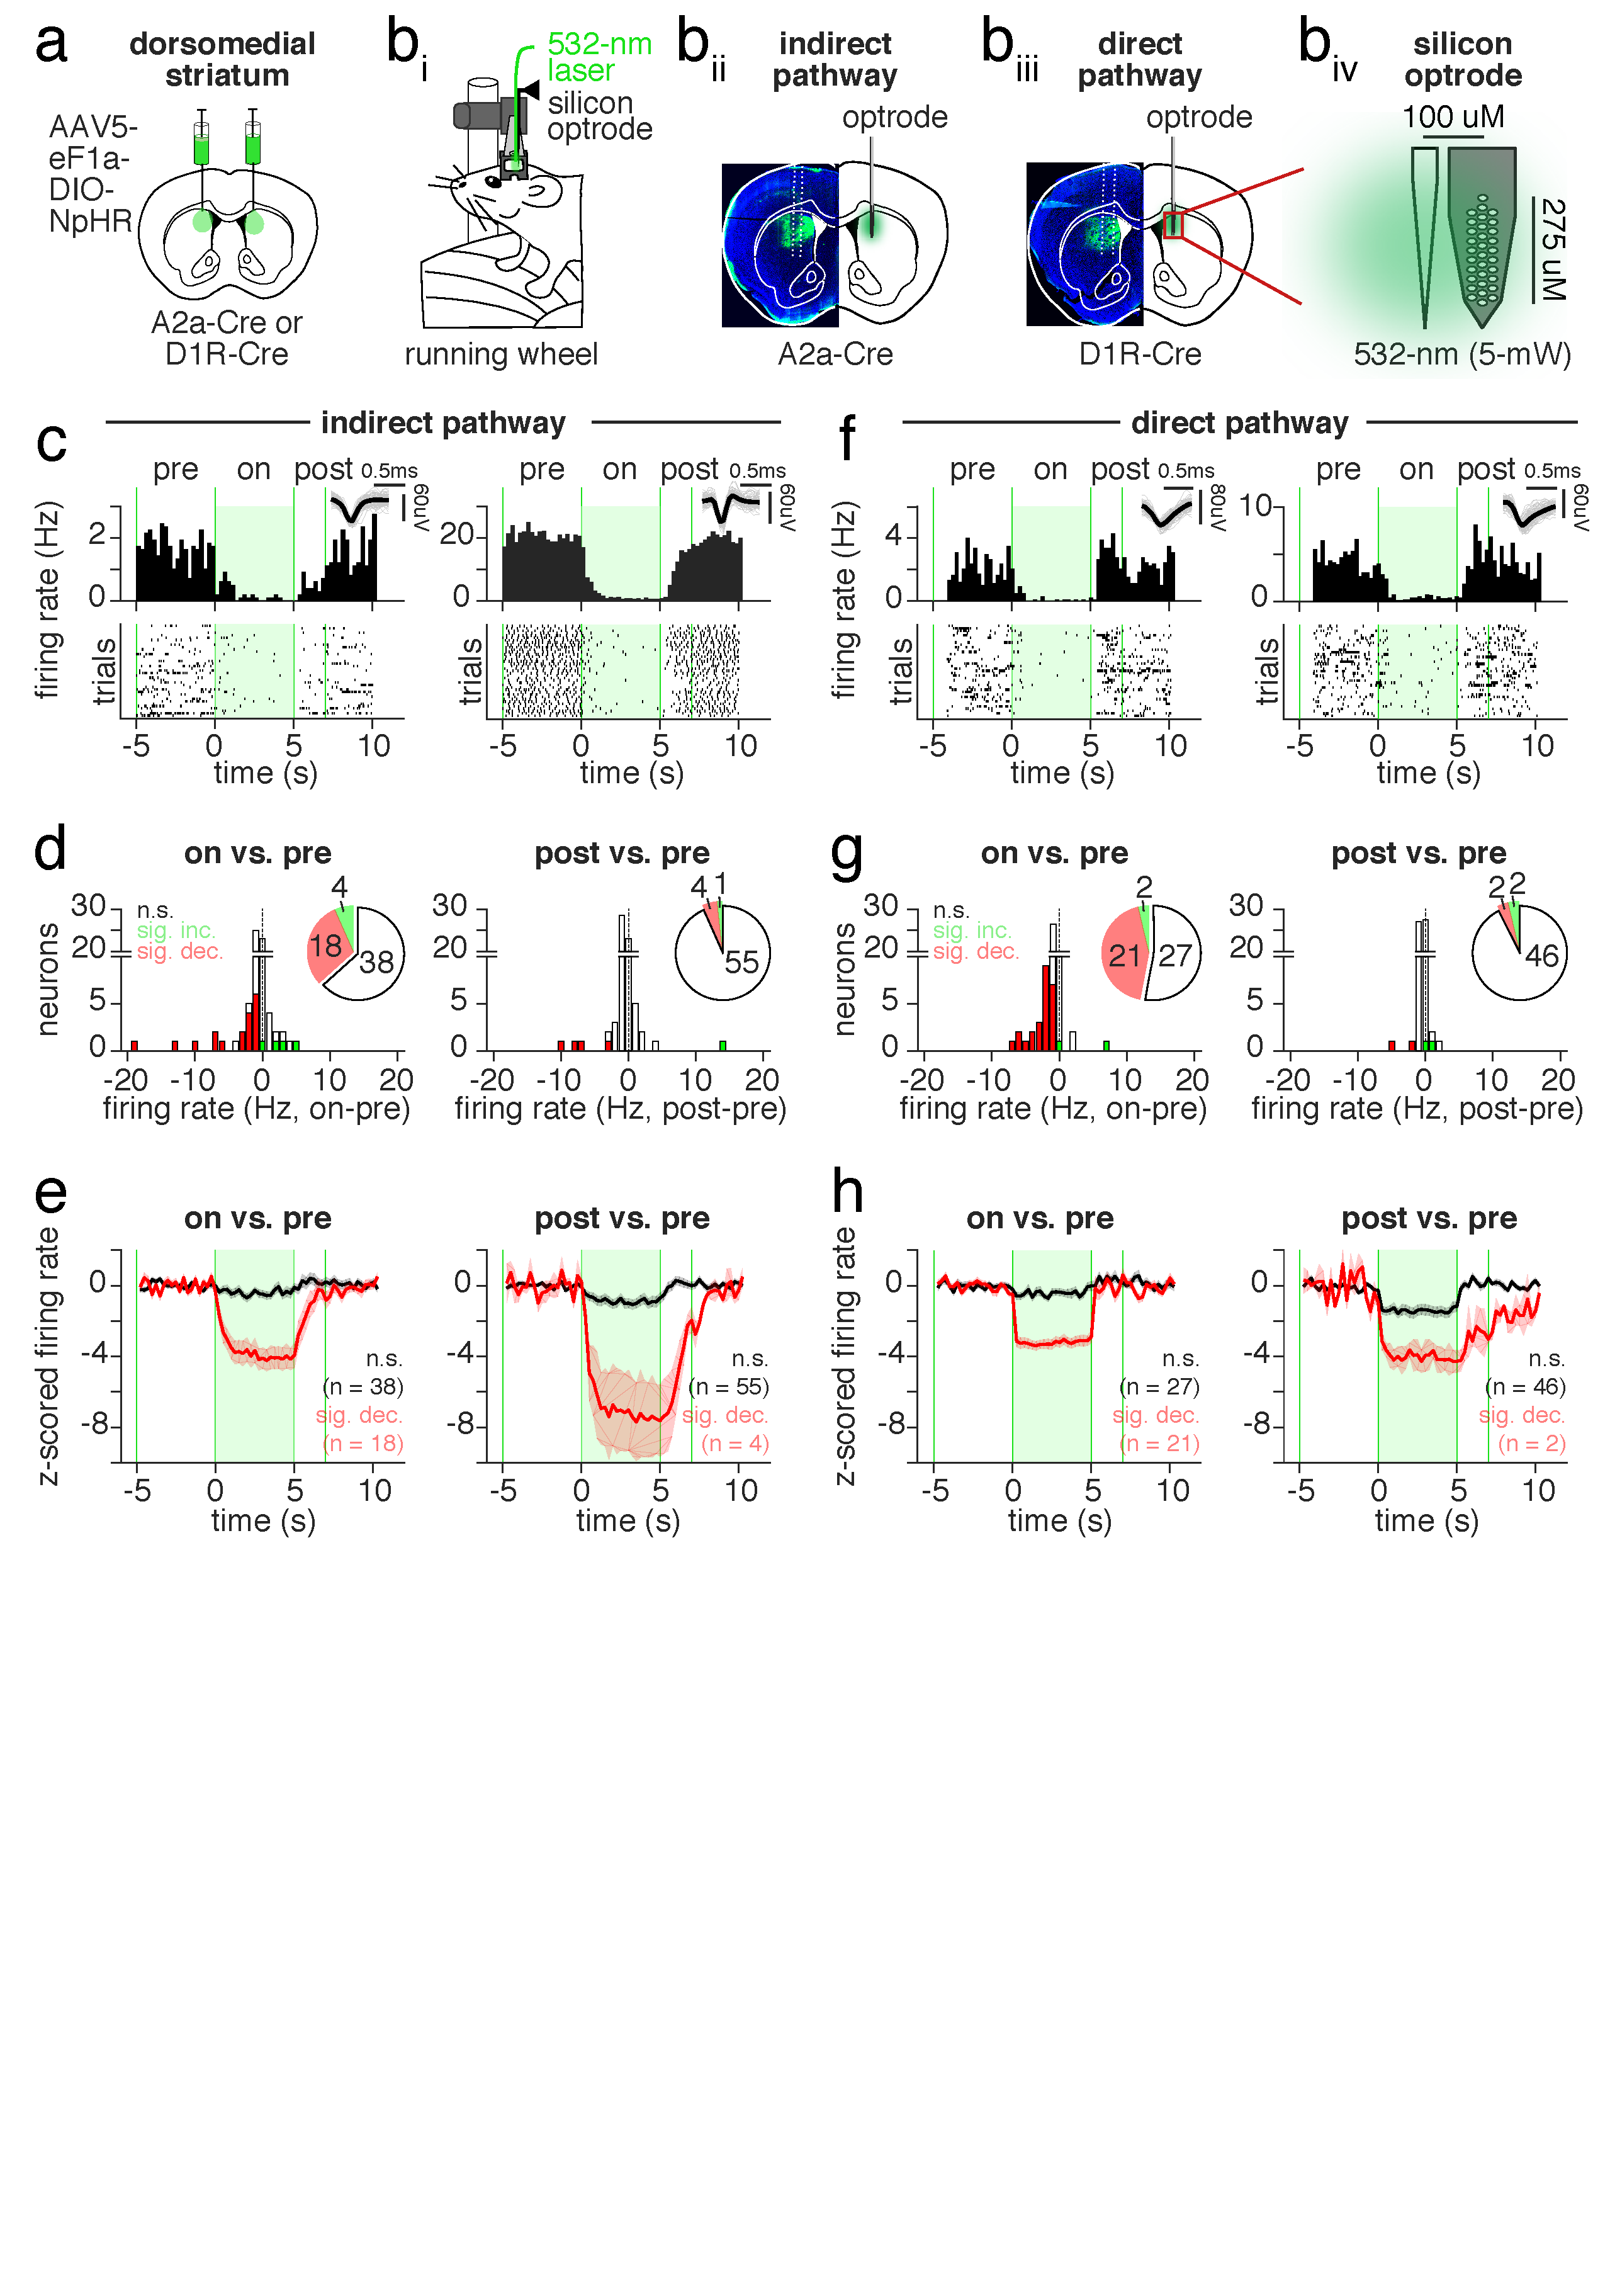
\includegraphics[width=0.90\linewidth]{ch7-appendix1/appendix1-figures/ExtData_Fig1.pdf}
    \caption[Optogenetic inhibition of DMS pathways is effective, generating little post-inhibitory rebound, nor excitation during the inhibition period]{\textbf{Optogenetic inhibition of DMS pathways is effective, generating little post-inhibitory rebound, nor excitation during the inhibition period.} (a) Schematic of viral delivery of AAV5-eF1a-DIO-NpHR to the dorsomedial striatum (DMS) of A2a-Cre or D1R-Cre mice. (b,i) Schematic of electrophysiological recording and laser delivery (532-nm, 5-mW) to the DMS in awake, head-fixed mice ambulating on a running wheel. (b,ii) Example recording electrode tracks and cre-dependent NpHR expression in an A2a-Cre mouse targeting the indirect pathway of the DMS. (b,iii) As in b,ii but in a D1R-Cre mouse targeting the DMS direct pathway. (b,iv) Schematic of silicon optrode recording tip, including tapered optical fiber coupled to a 32-channel silicon probe. (c) Two example peristimulus time histograms (PSTH) (top) and raster plots of trial-by-trial spike times (bottom) from single neurons recorded from the DMS of an A2a-Cre mouse. Inset at top displays average spike waveform (black) and 100 randomly sampled spike waveforms (grey) for each neuron. A trial consisted of 5-s without laser (pre, -5 to 0-s), 5-s of 532-nm light (5-mW) delivery (on, 0 to 5-s), followed by a 10-s ITI (40 trials per recording site). The first 2-s following laser offset (post, 5-7-s) was used to assess post-inhibitory effects. (d) Left: Histogram of change in average firing rate (on-pre, Hz) for all neurons (n = 60) recorded from the DMS of A2a-Cre mice (n = 3). Colors indicate non-significant (black, n = 38 neurons), significantly decreased }
    \label{fig:ap1:ext1}
  \end{center}
  \vspace{-1.5cm}
\end{figure}
\begin{figure}[t!]
\vspace{-7cm}
  \contcaption{(red, n = 18 neurons) or increased (green, n = 4 neurons) changes in firing rate determined via paired, two-tailed signrank comparison of average across-trial baseline (pre) or laser (on) firing rates. A Bonferroni-corrected significance threshold was used to account for multiple neuron comparisons (p < 0.00083, or p = 0.05/60 neuron comparisons). Right: same as left but for change in firing rate (post-pre, Hz): non-significant (n = 55 neurons), significantly decreased (n = 4) or increased (n = 1). Insets display pie-chart summaries of the proportion of non-significant (black unfilled), significantly decreased (red) or increased (green) neurons. (e) Left: Mean +/- SEM z-scored firing rate across all non-significantly modulated on vs pre (black, n = 38) or significantly decreased on vs pre (red, n = 18) neurons recorded from A2a-Cre mice. Right: same as left but for all non-significantly modulated post vs pre (black, n = 55) or significantly decreased post vs pre (red, n = 4) neurons. (f) Same as c but for example neurons recorded from the DMS of D1R-Cre mice. (g) Same as d but for all neurons (n = 50) recorded from the DMS of D1R-Cre mice (n = 2). Left (on-pre): non-significant (n = 27), significantly decreased (n = 21), or increased (n = 2). Right (post-pre): non-significant (n = 46), significantly decreased (n = 2) or increased (n = 2). A Bonferroni-corrected significance threshold was used to account for multiple neuron comparisons (p < 0.001, or p = 0.05/50 neuron comparisons). (h) same as e but for neurons recorded from the DMS of D1R-Cre mice.}% Continued caption
\end{figure}

\begin{figure}[t!]
  \begin{center}
    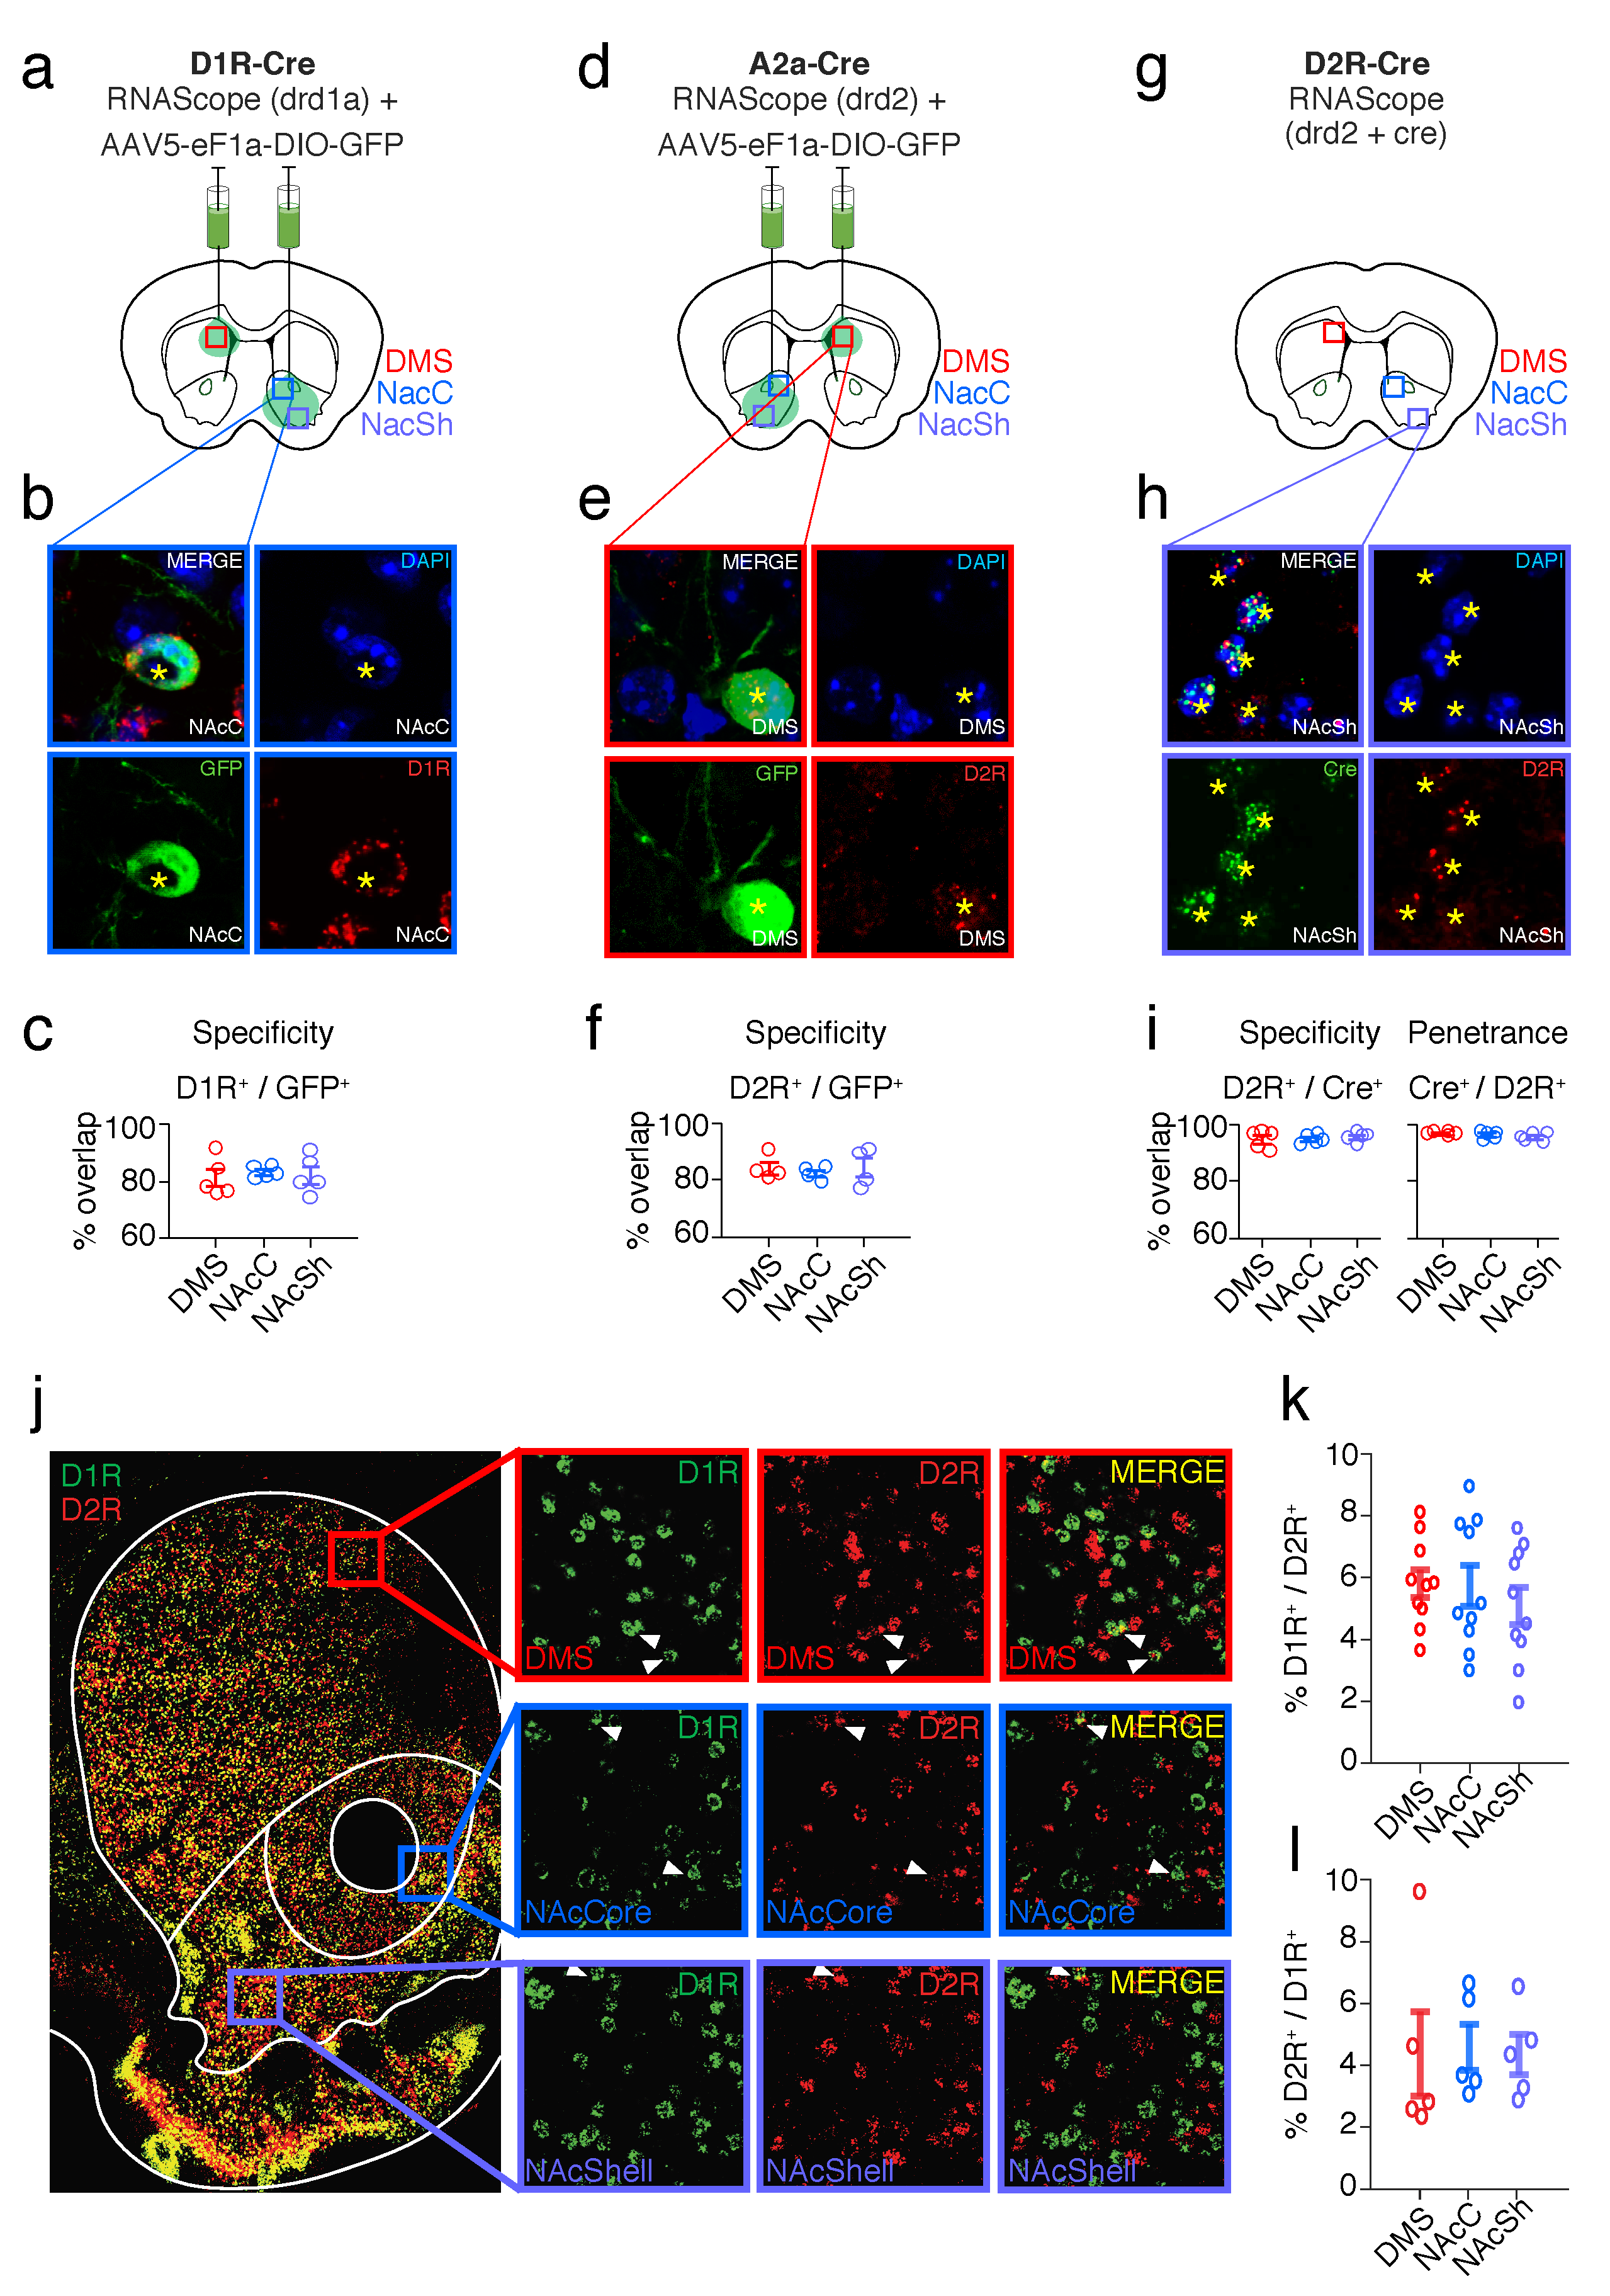
\includegraphics[width=0.90\linewidth]{ch7-appendix1/appendix1-figures/Supplementary_Fig1.pdf}
    \caption[Transgenic mouse lines faithfully report indirect and direct pathways across striatal subregions]{\textbf{Transgenic mouse lines faithfully report indirect and direct pathways across striatal subregions.}}
    \label{fig:ap1:supp2}
  \end{center}
  \vspace{-1.5cm}
\end{figure}
\begin{figure}[t!]
  \contcaption{(a) Schematic of viral delivery of AAV5-eF1a-DIO-GFP to the dorsomedial striatum (DMS) or nucleus accumbens (NAc) on opposite hemispheres of D1R-Cre mice. Red, blue, and purple squares denote representative areas for stereological quantification of viral co-expression with a drd1 mRNA probe (RNAScope) in the DMS, NAc core (NAcC), or NAc shell (NAcSh), respectively. (b) Example fluorescent confocal image (63x objective, 5x digital zoom) of the NAc core from a D1R-Cre mouse displaying virally- expressed GFP (green), drd1 mRNA (red), and DAPI (blue). (c) Percentage of GFP+ neurons co-expressing drd1 mRNA from 2 D1R-Cre mice across the DMS (red; n = 5 sections; 193 GFP+ neurons), NAcC (blue; n = 5 sections; 298 GFP+ neurons), or NacSh (purple; n = 4 sections; 312 GFP+ neurons). (d) Same as a, but for quantification of viral co-expression with a drd2 mRNA probe in A2a-Cre mice. (e) Same as b, but for an example image of the DMS from an A2a-Cre mouse and displaying drd2 mRNA (red). (f) Same as c, but for percentage of virally-expressed GFP+ neurons co-expressing drd2 mRNA in 2 A2a-Cre mice across the DMS (red; n = 4 sections; 312 GFP+ neurons), NAcC (blue; n = 4 sections; 326 GFP+ neurons), or NacSh (purple; n = 4 sections; 312 GFP+ neurons). (G) Same as A and D, but for quantification of co-expression of drd2 and cre mRNA in 2 D2R-Cre mice. (h) Same as b and e, but for an example image of the NAcSh from a D2R-Cre mouse and displaying cre mRNA (green) and drd2 mRNA (red). (i) Left: same as c and f, but for percentage of neurons with cre mRNA co-expressing drd2 mRNA in 2 D2R-Cre mice across the DMS (red; n = 5 sections; 1302 cre+ neurons), NAcC (blue; n = 5 sections; 1,104 cre+ neurons), or NacSh (purple; n = 4 sections; 1,187 cre+ neurons). Right: same as left but for neurons with drd2 mRNA co-expressing cre mRNA across DMS (red; n = 5 sections; 1,269 drd2+ neurons), NAcC (blue; n = 5 sections; 1,055 drd2+ neurons), or NacSh (purple; n = 5 sections; 1,114 cre+ neurons). Solid bars denote mean and s.e.m. throughout. (j) Example fluorescent confocal microscopy image of a coronal section from a DR2-Cre mouse that underwent fluorescent in situ hybridization with probes targeting drd1a and drd2 receptor mRNA. Left: 20x magnification tilescan spanning dorsal and ventral striatum. Right top: 63x confocal images of dorsomedial striatum (DMS, red square) and expression of drd1a mRNA (green), drd2 mRNA (red), and merged image of both (yellow). White triangles indicate co-expression of receptor probes in single neurons. Right middle: same as right top but for 63x confocal images of nucleus accumbens core (NAcC, blue square). Right bottom: same as right top but for 63x confocal images of nucleus accumbens shell (NAcSh, purple square). (k) Percentage of drd2+ neurons co-expressing drd1a mRNA from 2 D2R-Cre and 2 D1R-tdTomato mice in the DMS (red; n = 10 sections; 2,423 drd2+ neurons), NAcC (blue; n = 10 sections; 2,196 drd2+ neurons), or NacSh (purple; n = 10 sections; 2,220 drd2+ neurons). Circles indicate mean overlap from individual sections. (l) Same as k, but for percentage of drd1a+ neurons co-expressing drd2 mRNA from 2 D1R-tdTomato mice in the DMS (red; n = 5 sections; 868 drd1a+ neurons), NAcC (blue; n = 5 sections; 834 drd1a+ neurons), or NacSh (purple; n = 5 sections; 874 drd1a+ neurons). Throughout solid bars reflect mean +/- S.E.M. and transparent ‘o’ denote individual slice mean. Each staining was repeated on 2 independent samples (mice) per group with similar results.  }% Continued caption
\end{figure}

\begin{figure}[t!]
  \begin{center}
    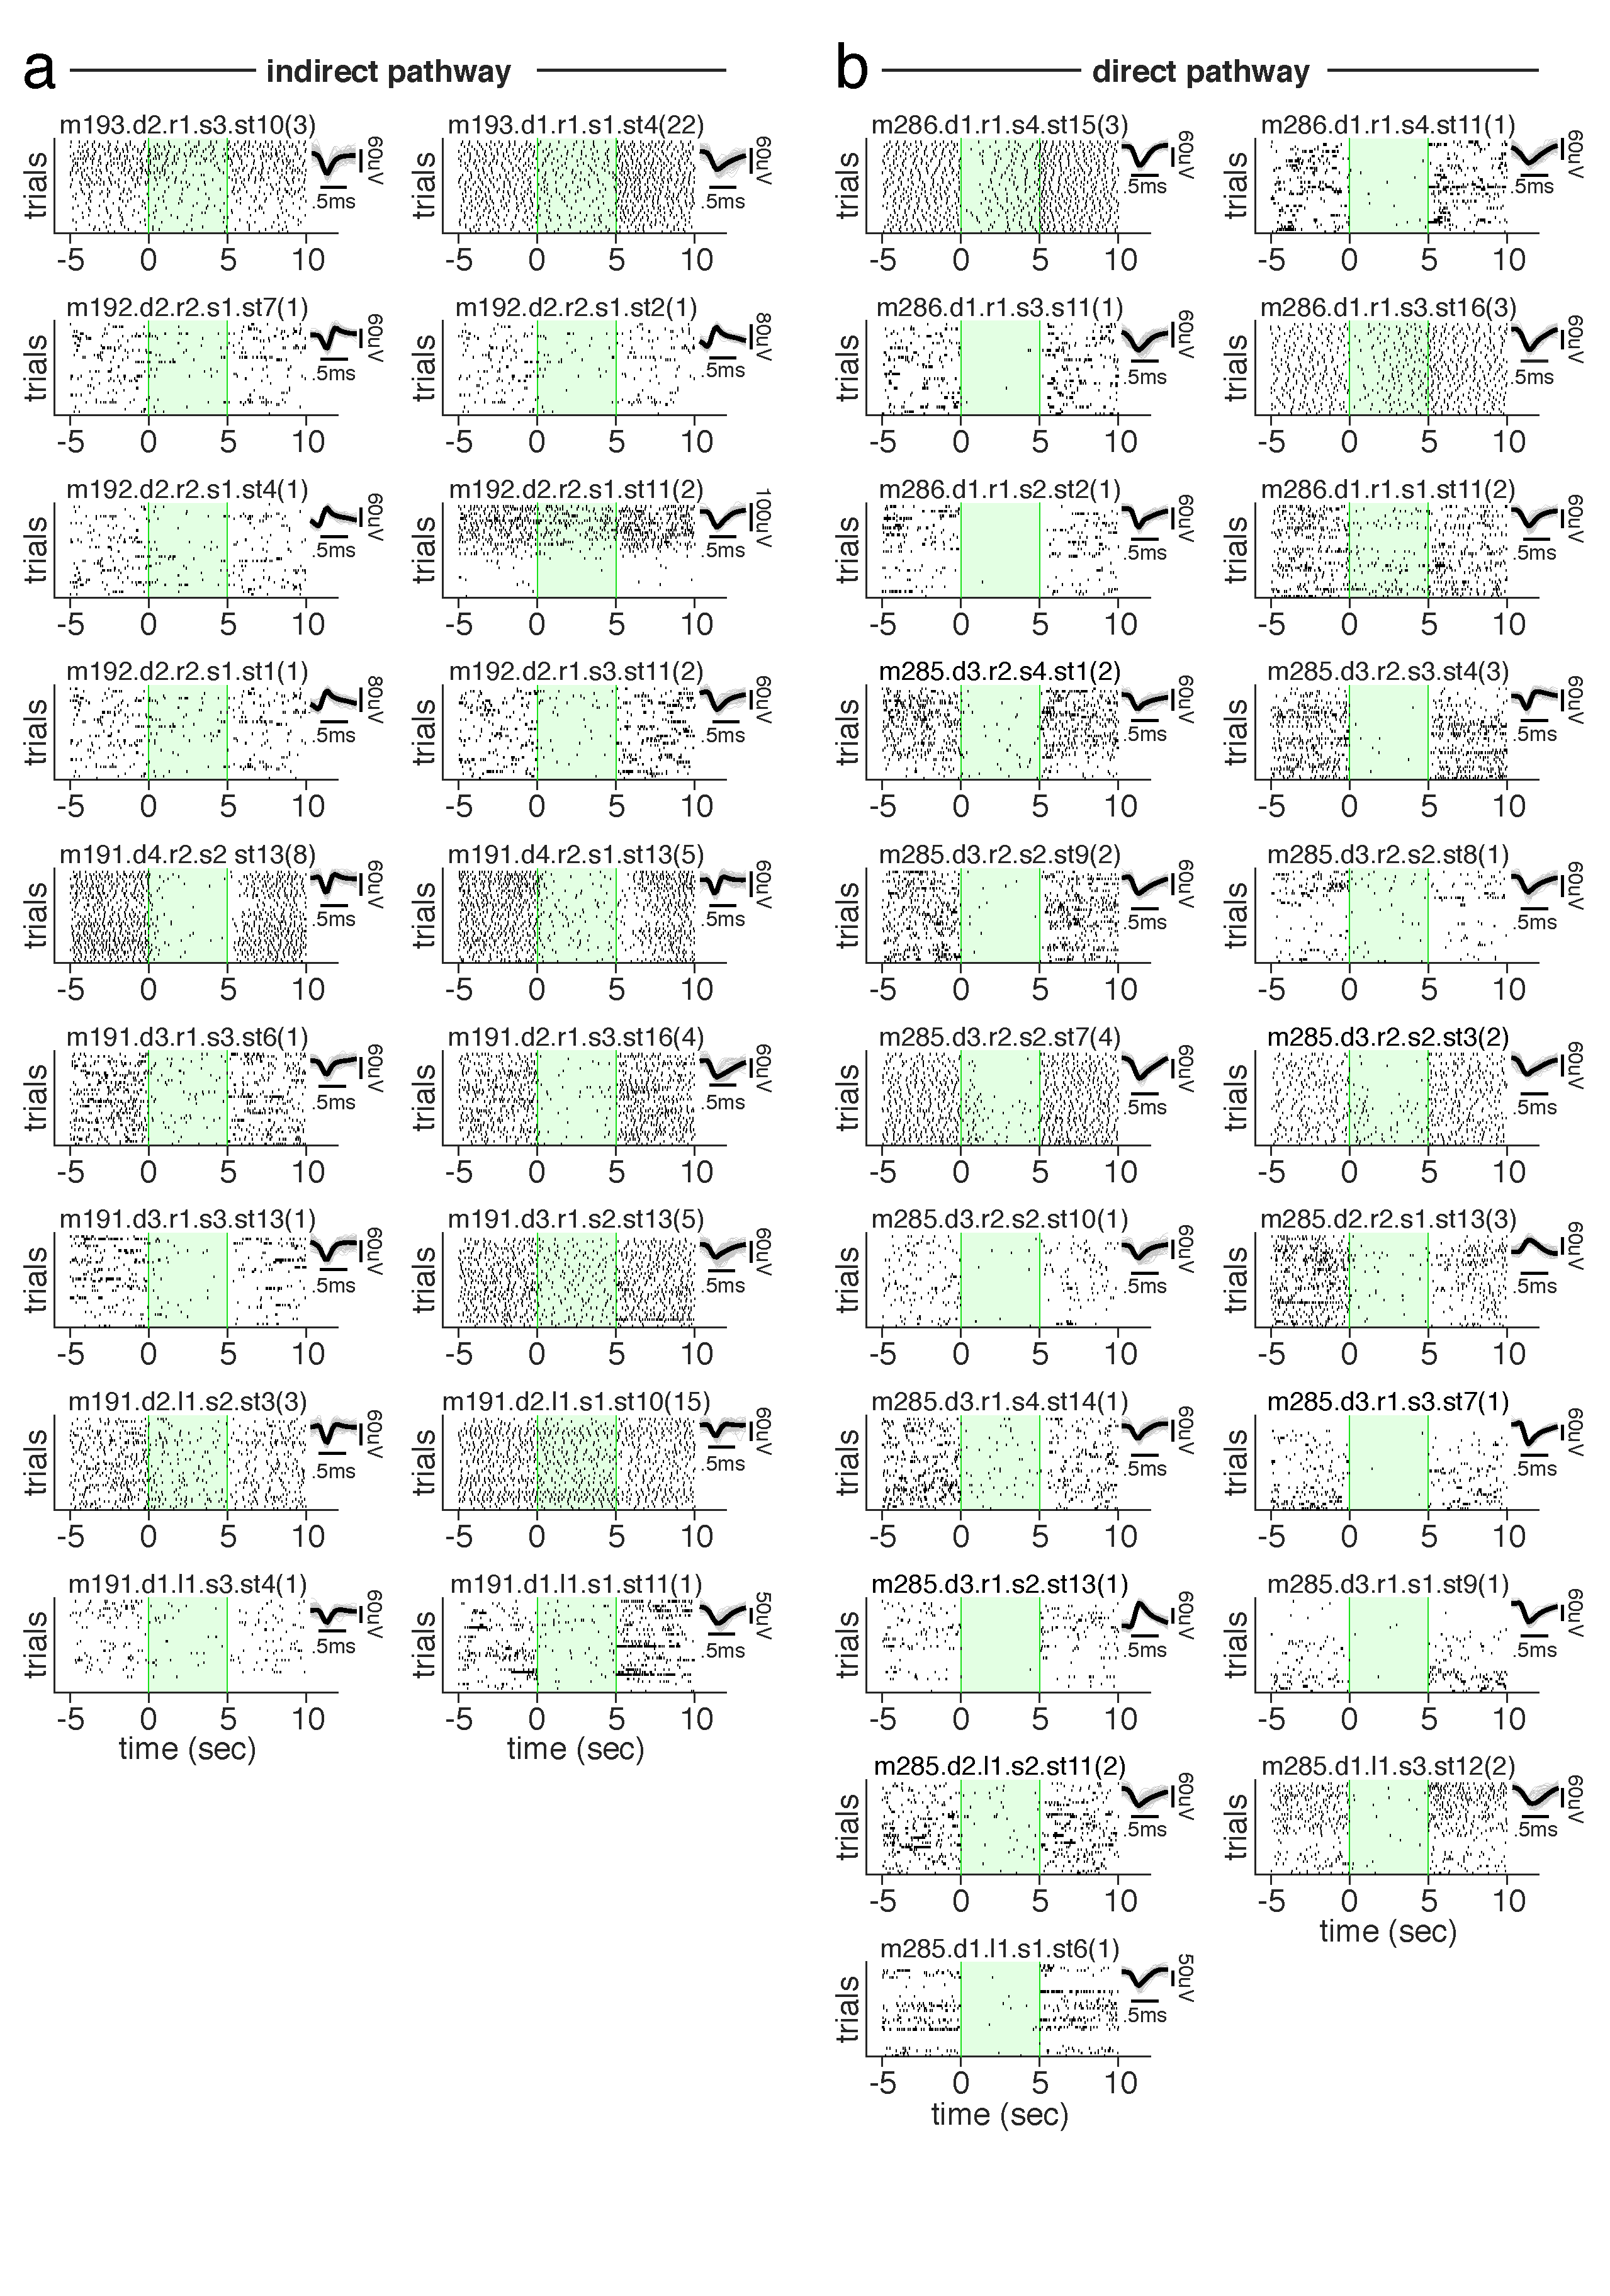
\includegraphics[width=0.90\linewidth]{ch7-appendix1/appendix1-figures/Supplementary_Fig2.pdf}
    \caption[Indirect and direct pathway inhibition of the DMS is stable across time]{\textbf{Indirect and direct pathway inhibition of the DMS is stable across time.} }
    \label{fig:ap1:ext1}
  \end{center}
  \vspace{-1.5cm}
\end{figure}
\begin{figure}[t!]
\vspace{-3cm}
  \contcaption{\textbf{}  (a) Trial-by-trial raster plots of single neuron spiking during laser off baseline (-5 to 0s), 532-nm  (5-mW)  laser delivery (0 to 5s), and post laser offset (5 to 10s) for all significantly inhibited neurons  (n = 18/60) recorded from A2a-Cre mice expressing Cre-dependent NpHR in the DMS. 40 total trials of laser sweeps per recording site (~15 minutes), ordered in time top to bottom. Individual neuron labels indicate: m (mouse), d (day of recording), r/l (right/left hemisphere and penetration number), s (site or depth of recording probe numbered ventral to dorsal), and st (probe stereotrode channel). Number in parenthesis indicates the number of spikes sub-sampled for display. Inset displays average (bold) and 100 randomly sampled spike waveforms (grey). (b) As in a but for all significantly inhibited neurons recorded from D1R-Cre mice expressing Cre-dependent NpHR in the DMS (n =21/50).}% Continued caption
\end{figure}

\chapter{Supplemental Materials for bestLDS Project\label{ch:appendix2}}

\section{Additional Tables}
\label{sec:appendix2:tables}

\begin{table*}[ht]
\setlength{\tabcolsep}{5pt}
\centering
\caption{\textbf{Generative parameters for simulated datasets.}}
\vspace{0.5cm}
\begin{tabular}{|p{1.5cm}||p{2.5cm}|p{2.2cm}|p{2.2cm}|p{2.2cm}|p{1.1cm}|p{0.4cm}|p{0.4cm}|p{0.4cm}|}
 \hline
 \multicolumn{9}{|c|}{\textbf{Simulated dataset parameters }} \\
 \hline
 \textbf{Dataset} & \textbf{A} & \textbf{B} & \textbf{C}  & \textbf{D} & \textbf{Q} & \textbf{q} & \textbf{p} & \textbf{m} \\
 \hline
 \textbf{A} &   eigenvalues in [.9,.99]  & orthonormal scaled by .1   & orthornormal scaled by .1 & orthonormal scaled by .1 & .1$I$ & 1 & 3 & 3 \\
 \textbf{B} &   eigenvalues in [.9,.99]  & orthonormal scaled by .1   & orthornormal scaled by .1 & orthonormal scaled by .1  & .1$I$ & 10 & 5 & 3 \\
  \textbf{C} &   eigenvalues in [.5, .9]  & orthonormal scaled by .1  & orthonormal scaled by 10 & orthonormal scaled by .1 & .1$I$ & 8 & 6 & 4 \\
  \textbf{D}    & rotation matrix with $\theta = \pi/48$ & orthonormal scaled by .1 &  orthonormal scaled by 1e4 & orthonormal scaled by .1 & $.0001I$ & 5 & 2 & 3 \\
   \textbf{E}    & rotation matrix with $\theta = \pi/2$ & orthonormal scaled by .1 &  orthonormal scaled by 1e4 & orthonormal scaled by .1  & $.1I$ & 5 & 2 & 3\\
    \textbf{F}    & eigenvalues in [.9,.99]  & orthonormal scaled by .1   & orthornormal scaled by .1 & orthonormal scaled by .1  & .1$I$ & 10 & 5 & 3 \\
    \textbf{G}    & rotation matrix with $\theta = \pi/400$  & scaled by .01   & scaled by .25 & scaled by .2  & .001$I$ & 1 & 2 & 3 \\
 \hline
\end{tabular}
\label{table:ap2:1}
\vspace{-0.3cm}
\end{table*}
\section{Additional Figures}
\label{sec:appendix2:figures}

\begin{figure*}[bh!]
\centering
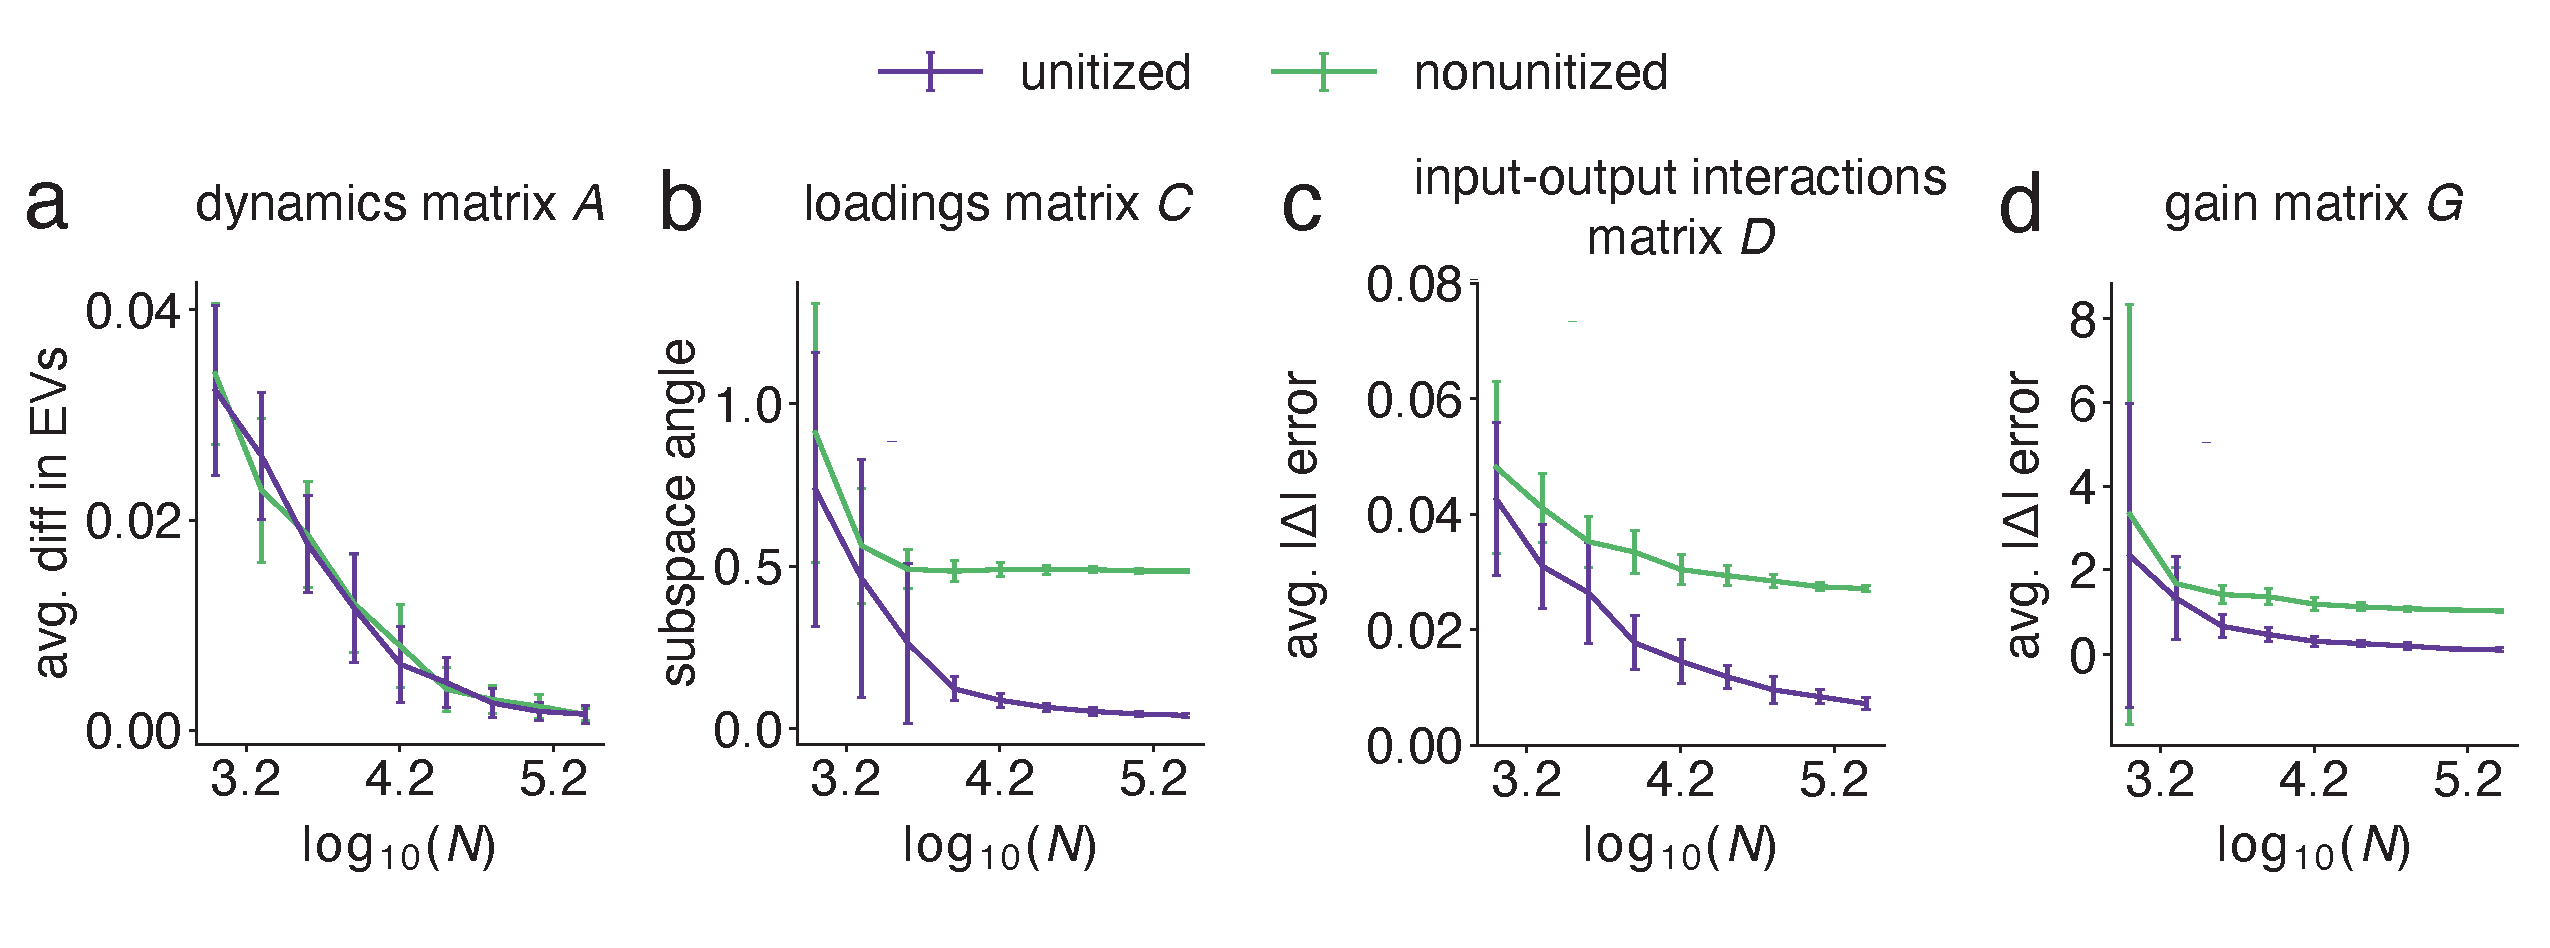
\includegraphics[width=0.90\textwidth]{ch4-bestlds/bestlds-figures/suppfig1.pdf}
\caption[Spectral estimator recovers simulation parameters in a variety of settings]{\textbf{Spectral estimator recovers simulation parameters in a variety of settings.} \textbf{(a)} Covariance matrix Cov$[y_{t+1}, y_{t}]$ showing the sample covariance of the binary observations $y$ (left), the covariance of $z$ obtained by converting the moments of $y$ (middle), and the ground truth covariance of $z$ (right) for a simulated dataset ($q = 30$, $p = 15$, $k =20$, $m=3$). Note that the transformed covariance closely matches the ground truth. \textbf{(b)} The singular value spectrum of the Hankel matrix computed at various settings of the Hankel size $k$. For all settings, only the top $p=5$ singular values are greater than zero. \textbf{(c-e)} Recovery error for bestLDS inferred parameters vs. training data size for a low-dimensional dataset with $ k=3$. For (c) we use the average absolute difference in the eigenvalues as the recovery error, and for (d) and (e) we use the average absolute elementwise difference. \textbf{(f-i)} Recovery error for bestLDS inferred parameters vs. training data size for a high-dimensional dataset with $k=10$. For (g) the recovery error is the angle of the }
%\vspace{-0.5cm}
\label{fig:ap2:1}
\end{figure*}

\begin{figure*}[ht]
\centering
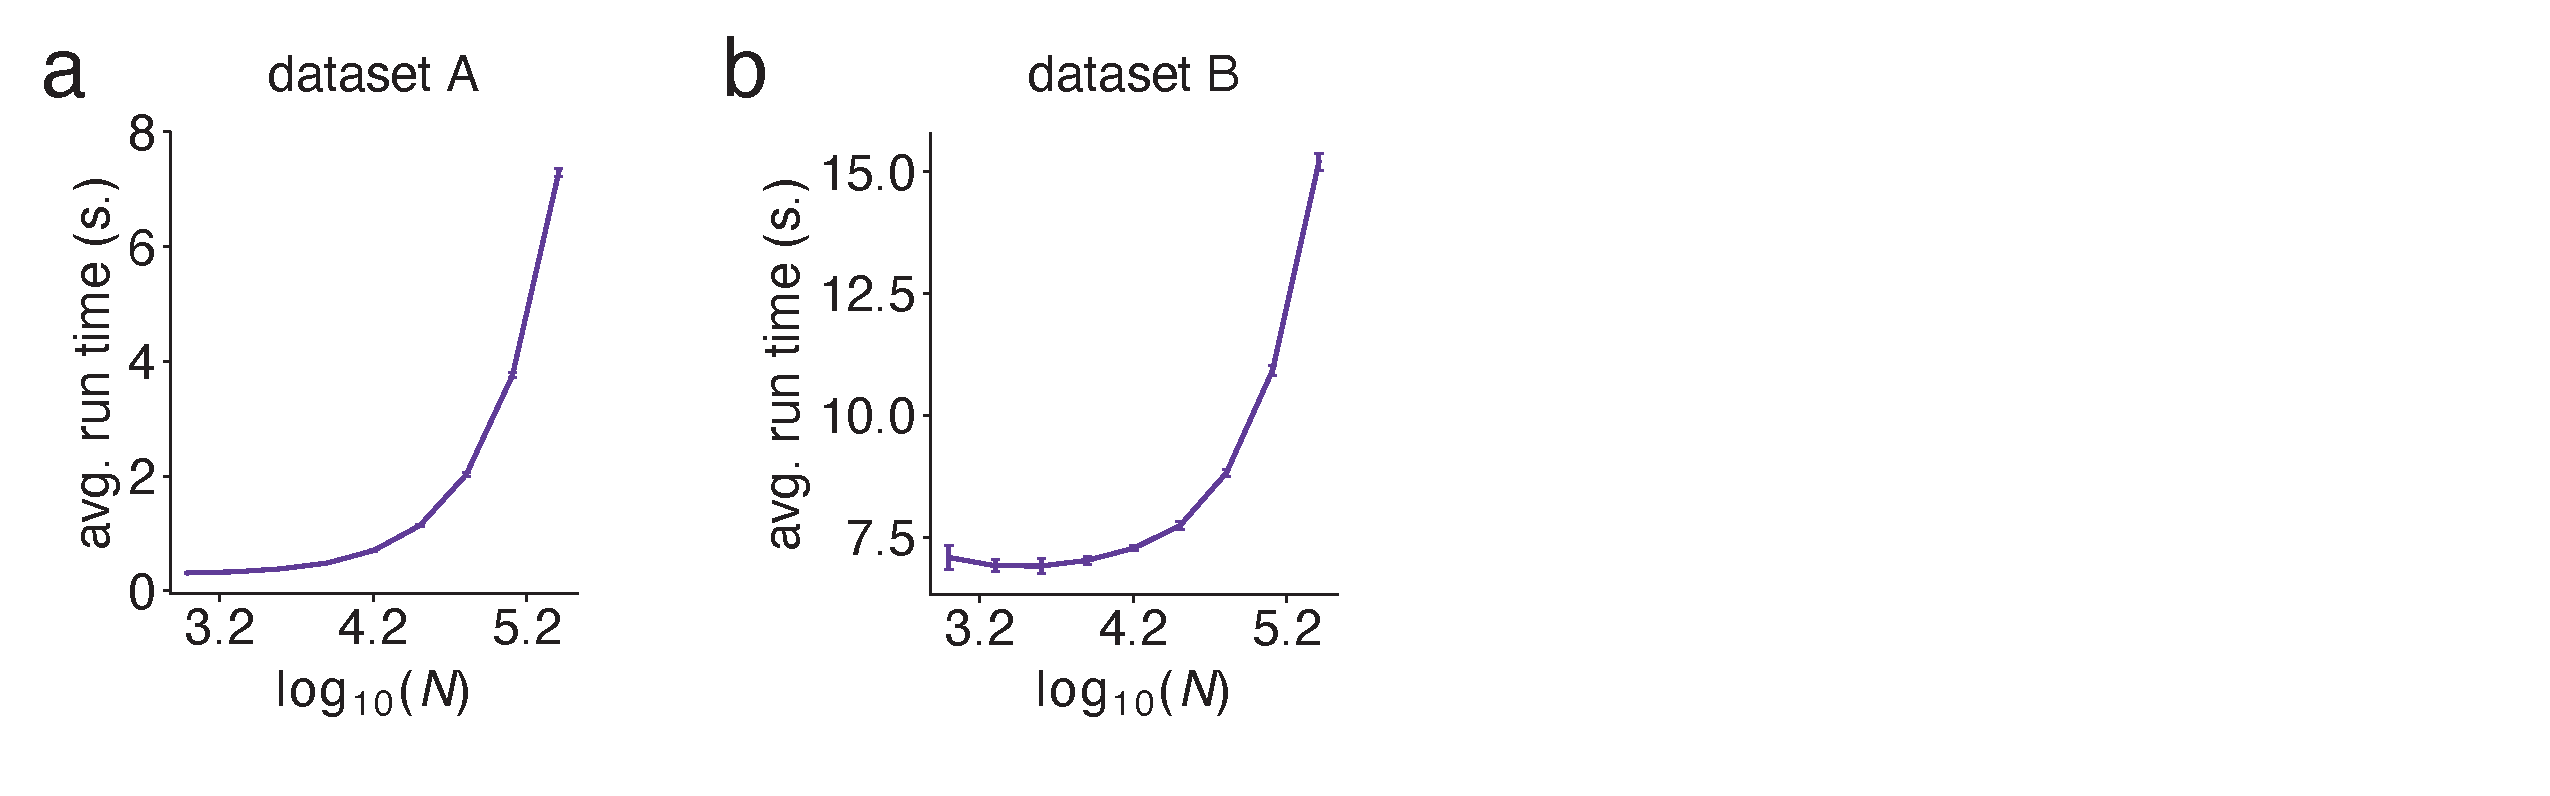
\includegraphics[width=0.90\linewidth]{ch4-bestlds/bestlds-figures/suppfig2.pdf}
\caption[bestLDS run time as a function of dataset size]{\textbf{bestLDS run time as a function of dataset size.}}
\label{fig:ap2:2}
\vspace{-0.5cm}
\end{figure*}

\begin{figure*}[t]
\centering
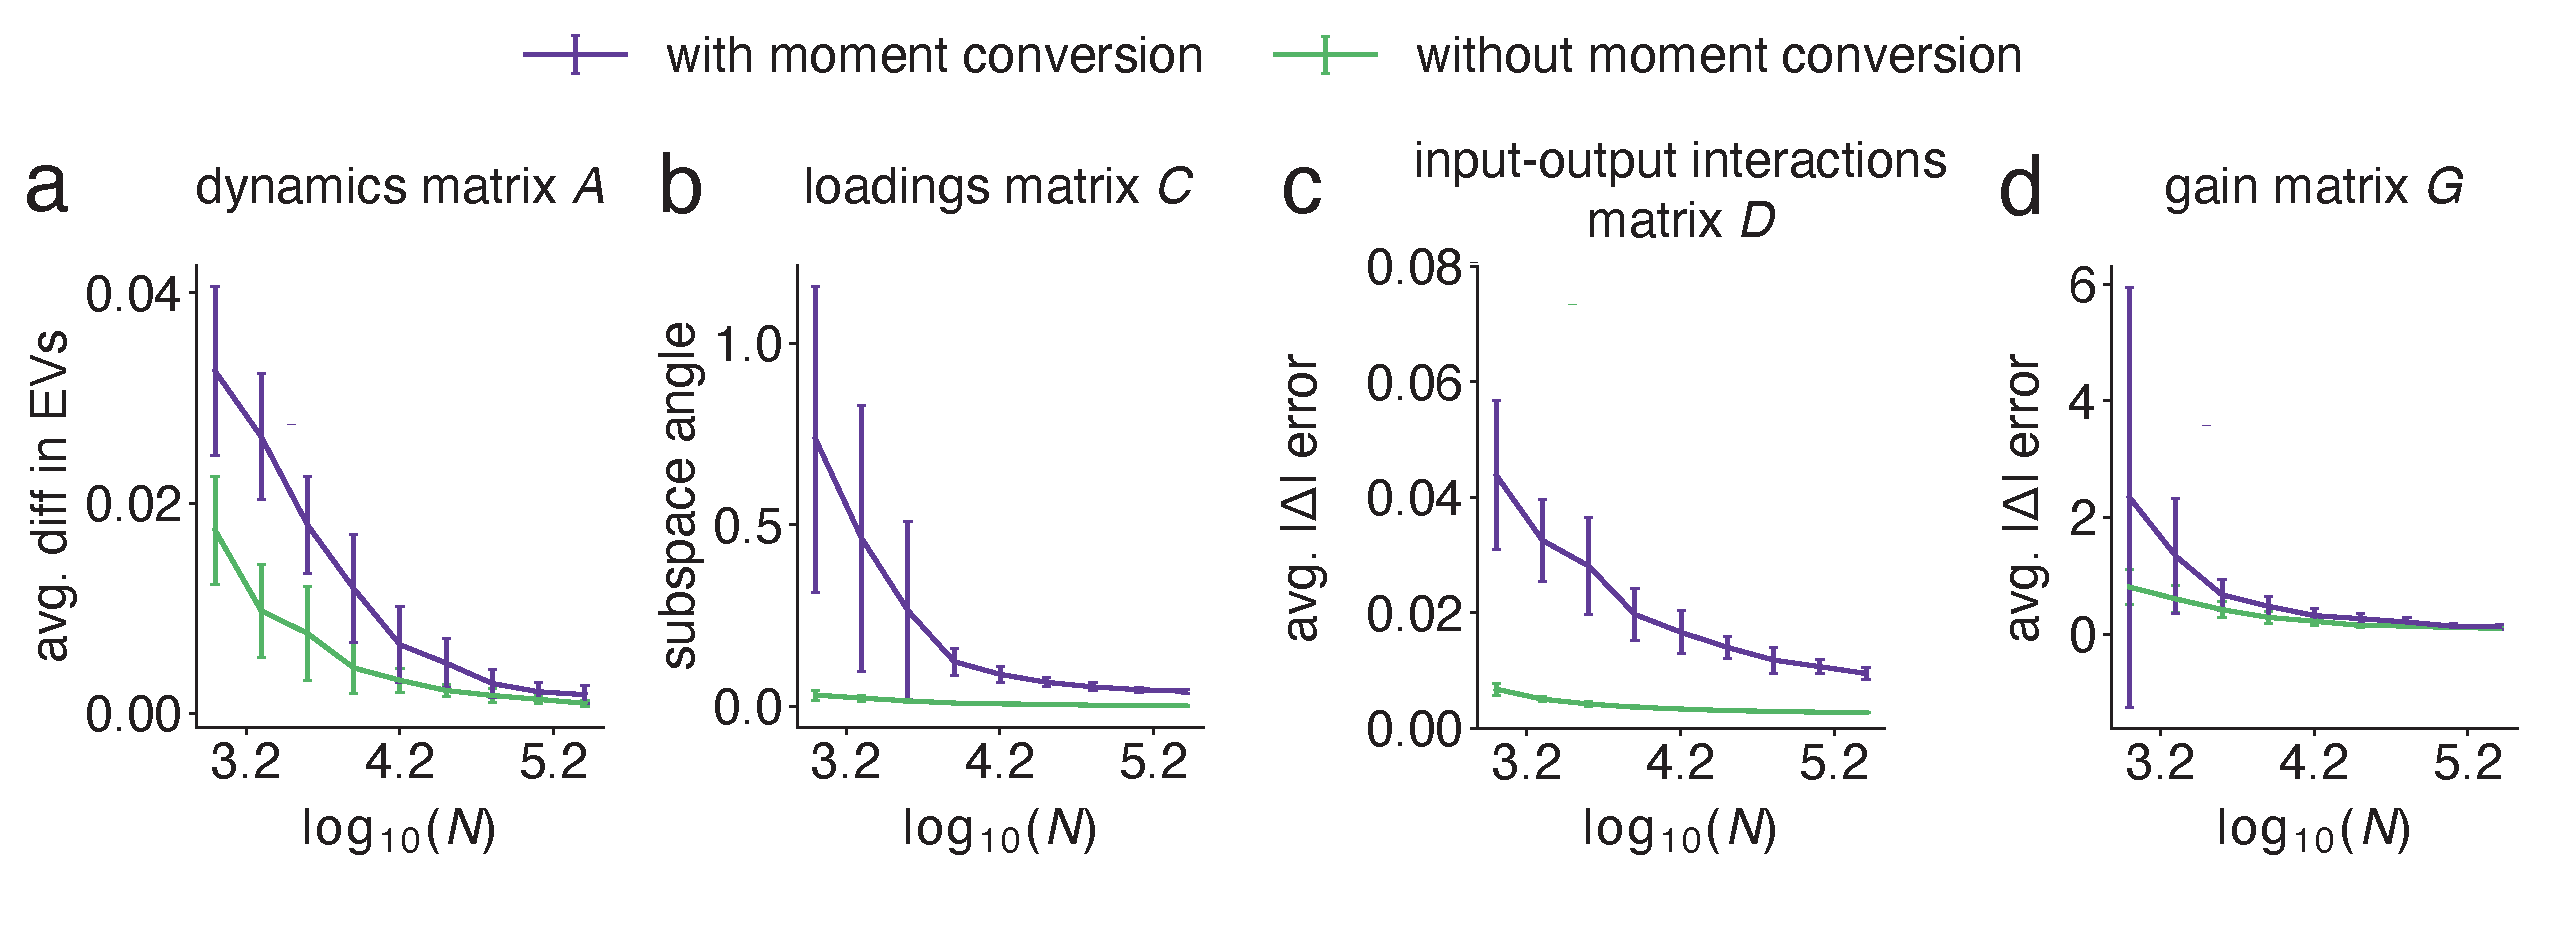
\includegraphics[width=0.90\linewidth]{ch4-bestlds/bestlds-figures/suppfig3.pdf}
\caption[bestLDS underperforms compared to a model that has direct access to $z$]{\textbf{bestLDS underperforms compared to a model that has direct access to $z$.} \textbf{(a-d)} Average recovery error for bestLDS inferred parameters (``with moment conversion'') vs. running N4SID directly on $z$ (``without moment conversion'').}
\label{fig:ap2:3}
\vspace{-0.5cm}
\end{figure*}

\begin{figure*}[ht]
\centering
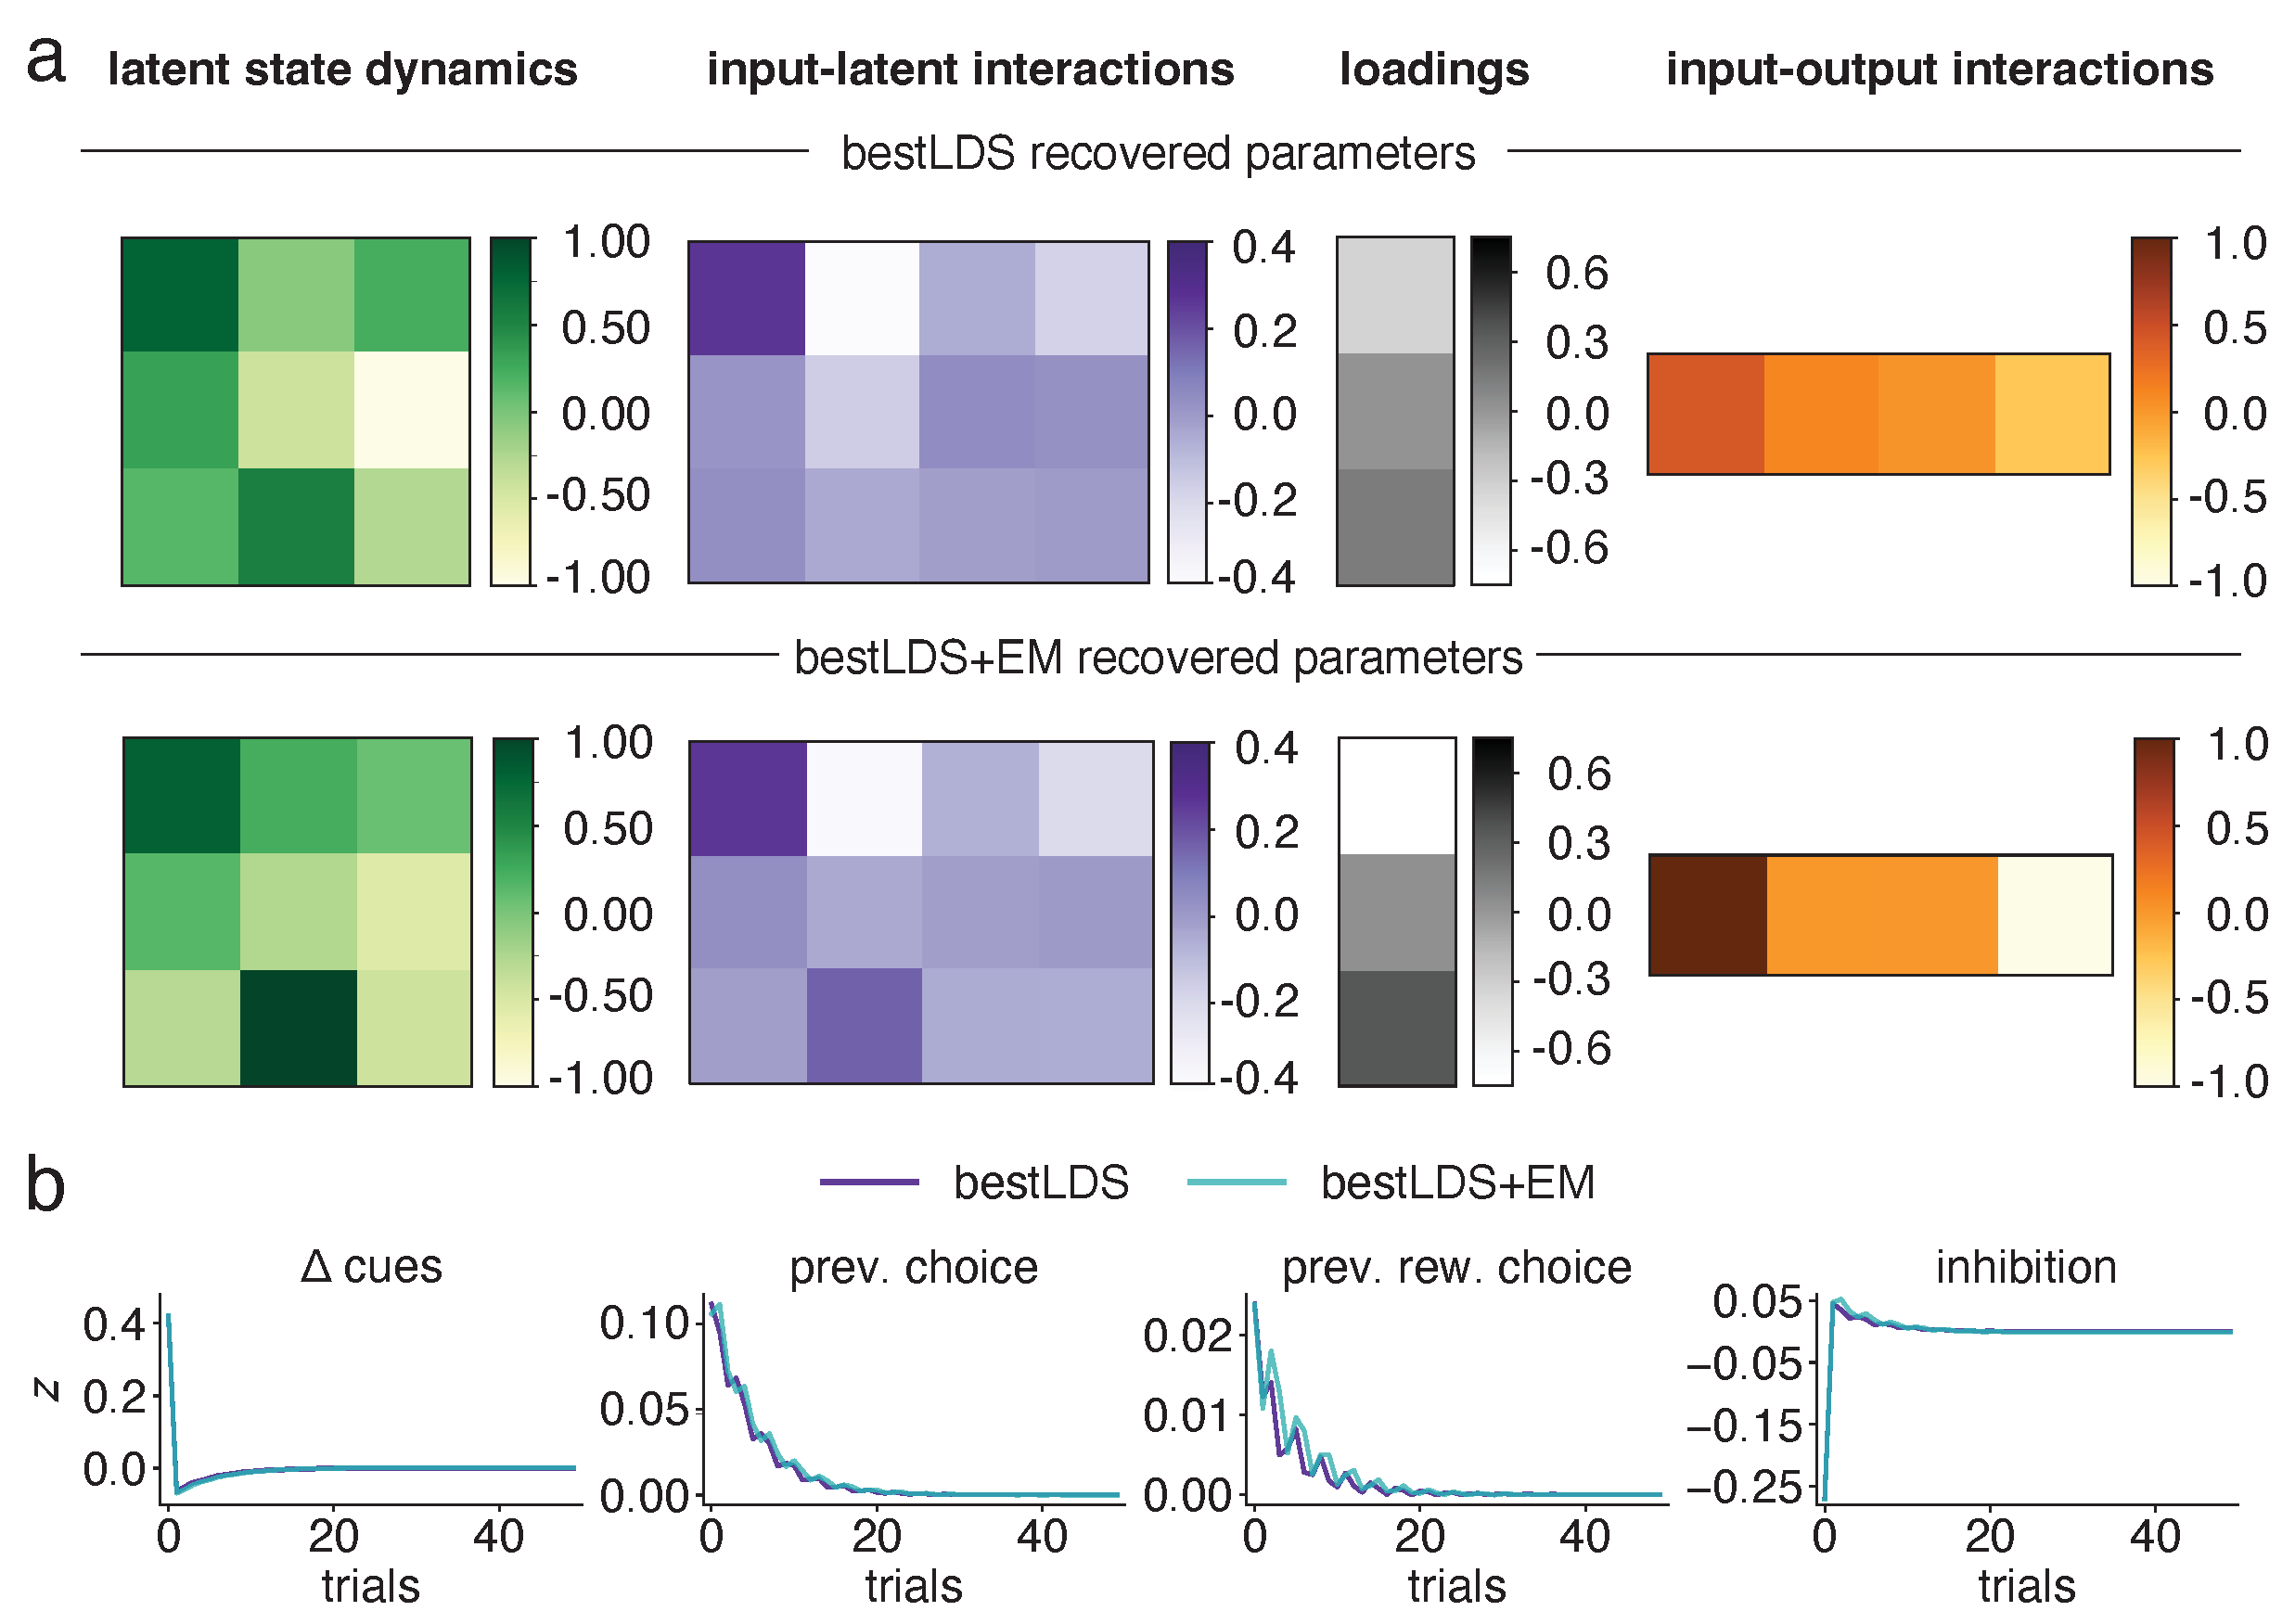
\includegraphics[width=0.95\linewidth]{ch4-bestlds/bestlds-figures/suppfig4.pdf}
\caption[bestLDS recovered parameters closely match the inferred parameters using EM with bestLDS initializations]{\textbf{bestLDS recovered parameters closely match the inferred parameters using EM with bestLDS initializations.} \textbf{(a)} The recovered parameters using bestLDS (top) and bestLDS+EM (bottom).   \textbf{(b)} Impulse responses for each of the fitted systems. In each subplot, data has been simulated noiselessly with a unit input in the indicated dimension.}
\label{fig:ap2:4}
%\vspace{-0.5cm}
\end{figure*}



% Make the bibliography single spaced
\singlespacing
%\bibliographystyle{plain}

% add the Bibliography to the Table of Contents
\cleardoublepage
\ifdefined\phantomsection
  \phantomsection  % makes hyperref recognize this section properly for pdf link
\else
\fi
\addcontentsline{toc}{chapter}{Bibliography}

% include your .bib file
\bibliography{references}

\end{document}

